\documentclass{article}

\usepackage[utf8]{inputenc}

\usepackage[english]{babel}
\usepackage{microtype}
\usepackage{graphics, graphicx}
\usepackage[a4paper,top=3cm,bottom=3cm,left=3cm,right=3cm]{geometry}
\usepackage{amsmath, amssymb, mathrsfs}
\usepackage{booktabs}
\usepackage{fancyvrb}
\usepackage{hyperref}
\usepackage{url}


\title{\textbf{Mapper}}
\date{June 2018}
\author{Francesca Sellarione \and Beatrice Beco}


\begin{document}
\maketitle
\tableofcontents
\newpage

\section{Introduction}
The mapper module aims to provide the tools needed to apply both dimension-independent affine transformations and general simplicial maps to geometric objects and assemblies developed within the LAR scheme.

A large number of surfaces and primitives solids are definable using the map function and the local parametrizations:

\begin{enumerate}
\item Primitive one-dimensional objects: 
\begin{itemize}
\item larCircle - Circle centered in the origin
\item larHelix - Helix curve about the $z$ axis
\end{itemize}
\item Primitive two-dimensional objects:
\begin{itemize}
\item larDisk - Disk centered in the origin
\item larHelicoid - Helicoid about the $z$ axis 
\item larRing - Ring centered in the origin
\item larCylinder - Cylinder surface with $z$ axis
\item larSphere - Spherical surface of given radius
\item larToroidal - Toroidal surface of given radiuses
\item larCrown - Half-toroidal surface of given radiuses
\end{itemize}
\item Primitive three-dimensional objects: 
\begin{itemize}
\item larBox - Solid box of given extreme vectors
\item larBall - Solid Sphere of given radius
\item larRod - Solid cylinder of given radius and height
\item larHollowCyl - Hollow cylinder of given radiuses and height
\item larHollowShere - Hollow sphere of given radiuses
\item larTorus - Solid torus of given radiuses
\item larPizza - Solid pizza of given radiuses 
\end{itemize}
\end{enumerate}
%=================================================================================

\newpage
\section{Implementation}

\subsection{External functions used}

\paragraph{t function}

\begin{verbatim}
@everywhere function t(args)
    d = length(args)
    mat = eye(d+1,d+1)
    for k in 1:d
        mat[k,d+1] = args[k]
    end
    return mat
end
\end{verbatim}

\paragraph{Example:}
The \verb!t([1,2,3])! function gives as output:
\[
\begin{bmatrix}
1.0 & 0.0 & 0.0 & 1.0 \\
0.0 & 1.0 & 0.0 & 2.0 \\
0.0 & 0.0 & 1.0 & 3.0 \\
0.0 & 0.0 & 0.0 & 1.0
\end{bmatrix}
\]

%---------------------------------------------------------------------------------
\paragraph{s function}

\begin{verbatim}
@everywhere function s(args)
    d = length(args)
    mat = eye(d+1,d+1)
    for k in 1:d
        mat[k,k] = args[k]
    end
    return mat
end
\end{verbatim}

\paragraph{Example:}
The \verb!s([1,2,3])! function gives as output:
\[
\begin{bmatrix}
1.0 & 0.0 & 0.0 & 0.0 \\
0.0 & 2.0 & 0.0 & 0.0 \\
0.0 & 0.0 & 3.0 & 0.0 \\
0.0 & 0.0 & 0.0 & 1.0
\end{bmatrix}
\]

%---------------------------------------------------------------------------------
\paragraph{larApplyMapper}

\begin{verbatim}
@everywhere function larApplyMapper(affineMatrix)
    function larApplyMapper0(model)
        if length(model) == 2 
            V,CV = model
        elseif length(model) == 3
            V,CV,FV = model 
        end
        V = *(affineMatrix,vcat(V,transpose(fill(1.0,size(V,2)))))
        if length(model) == 2 
            return V[1:size(V,1)-1,:], CV
        elseif length(model) == 3
            return V[1:size(V,1)-1,:],CV,FV 
        end
        return larApplyMapper0
    end
end
\end{verbatim}

\paragraph{Example:} A series of Julia commands:\\
\verb!julia> model=larCircle()(3)!\\
\verb!julia> V,CV=model!\\
\verb!julia> V!\\
\verb!2x4 Array{Float64,2}:!
\[
\begin{bmatrix}
1.0 & -0.5 & -0.5 & 1.0 \\
0.0 & 0.866025 & -0.866025 & -2.44929e-16
\end{bmatrix}
\]
\verb!julia> vcat(V,transpose(fill(1.0,size(V,2))))!\\
\verb!3x4 Array{Float64,2}:!
\[
\begin{bmatrix}
1.0 & -0.5 & -0.5 & 1.0 \\
0.0 & 0.866025 & -0.866025 & -2.44929e-16 \\
1.0 & 1.0 & 1.0 & 1.0
\end{bmatrix}
\]

With \verb!*(affineMatrix,vcat(V,transpose(fill(1.0,size(V,2)))))! it's calculated the rows for columns product between an affine matrix and the matrix displayed above.

With \verb!V[1:size(V,1)-1,:]! the matrix is returned without the last row.\\\\
\verb!julia> affineMatrix=s([1,2])!\\
\verb!3x3 Array{Float64,2}:!
\[
\begin{bmatrix}
1.0 & 0.0 & 0.0  \\
0.0 & 2.0 & 0.0  \\
1.0 & 0.0 & 1.0 
\end{bmatrix}
\]\\
\verb!julia> V=*(affineMatrix,vcat(V,transpose(fill(1.0,size(V,2)))))!\\
\verb!3x4 Array{Float64,2}:!
\[
\begin{bmatrix}
1.0 & -0.5 & -0.5 & 1.0  \\
0.0 & 1.73205 & -1.73205 & -4.89850e-16 \\
1.0 & 1.0 & 1.0 & 1.0
\end{bmatrix}
\]\\
\verb!julia> V[1:size(V,1)-1,:]!\\
\verb!2x4 Array{Float64,2}:!
\[
\begin{bmatrix}
1.0 & -0.5 & -0.5 & 1.0  \\
0.0 & 1.73205 & -1.73205 & -4.89850e-16 \\
\end{bmatrix}
\]

%---------------------------------------------------------------------------------
\paragraph{approxVal}
\begin{verbatim}
@everywhere function approxVal(PRECISION)
    function approxVal0(value)
        out = round(value*(10^(PRECISION)))/10^(PRECISION)
        if out == -0.0
            out = 0.0
        end
        return out 
    end
    return approxVal0
end
\end{verbatim}

This function approximates the number in the second argument to the number of decimal digits in the first argument. For example, \verb!approxVal(4)(1.234566)! returns \verb!1.2345!.

%---------------------------------------------------------------------------------
\paragraph{larSimplexGrid1}

\begin{verbatim}
@everywhere function larSimplexGrid1(shape)
    model = [[]],[[0]]
    for item in shape
        model = larExtrude1(model,fill(1,item))
    end
    V,CV = model
    V = hcat(V...)
    return V,CV
end

@everywhere function larExtrude1(model,pattern)
    V,FV = model
    d,m = length(FV[1]), length(pattern)
    coords = collect(cumsum(append!([0],abs.(pattern))))
    offset,outcells,rangelimit = length(V),[],d*m
    for cell in FV  
        tube = [v+k*offset for k in range(0,m+1) for v in cell]
        cellTube = [tube[k:k+d] for k in range(1,rangelimit)]
        outcells = vcat(outcells,reshape(cellTube,d,m))
    end
    cellGroups = []
    for i in 1:size(outcells,2)
        if pattern[i]>0
            cellGroups = vcat(cellGroups,outcells[:,i])
        end
    end
    outVertices = [vcat(v,[z]) for z in coords for v in V]
    outModel = outVertices,cellGroups
end
\end{verbatim}

%=================================================================================================================
For each function  the Python code of the original function, the Julia source of the sequential translation and the Julia source for the parallel translation will follow.

\subsection{larCircle}

\paragraph{Python}
\begin{Verbatim}[tabsize=4]
def larCircle(radius=1.,angle=2*PI,dim=1):
	def larCircle0(shape=36):
        domain = larIntervals([shape])([angle])
        V,CV = domain
        x = lambda p : radius*COS(p[0])
        y = lambda p : radius*SIN(p[0])
        return larMap([x,y])(domain,dim)
    return larCircle0	
\end{Verbatim}

\paragraph{Julia}
\begin{verbatim}
function larCircle(radius=1.,angle=2*pi)
    function larCircle0(shape=36)
        V,CV = LARLIB.larCuboids([shape])
        V = (angle/shape)*V
        W = hcat(map(u->[radius*cos(u); radius*sin(u)], V)...)
        return W,CV
    end
    return larCircle0
end
\end{verbatim}

The \textbf{larCircle} function creates circles centered in the origin using radius and angle from input. Using the $larCuboids()$ function, contained in the LARLIB library, a domain shape is given in input and a cuboidal complex is created. This complex will be modified using the $map$ function to apply the desired parametrization to the coordinates of each vertex.

In such case, the local parametrization used is:
$$f(u) = (radius*cos(u),radius*sen(u)),$$
where $u \in [0,angle]$.

In general, the $map$ function has the following syntax: $$\verb!map(f, c...) -> collection!;$$
In this case $f$ is an "anonymous function" $$\verb!u->[radius*cos(u); radius*sin(u)]!$$ which is applied to the coordinates of the vertices contained in the V collection.

Thus a new set of vertices is created; the coordinates are disposed vertically in a matrix using the $$\verb!hcat(A...)!$$ function.

\paragraph{Visualization examples}

\begin{verbatim}
using LARLIB
using LARVIEW

using PyCall
@pyimport larlib as p
\end{verbatim}

\begin{verbatim}
V,CV = larCircle()()
V
CV
LARVIEW.viewexploded(V,CV)
\end{verbatim}

\begin{figure}[htbp] 
\centering 
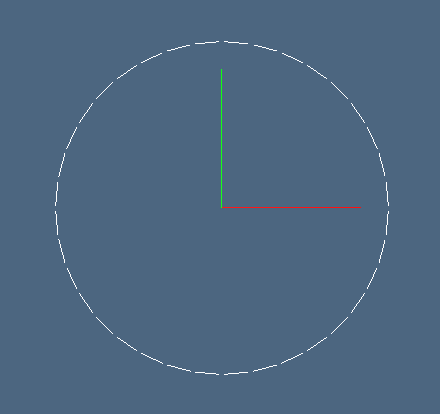
\includegraphics[scale=.36]{larCircle.png}
\caption{Circle centered in the origin with unit radius.}
\end{figure}


\paragraph{Test\\}

Tests are an integrating part of the usual activities of the developers, because they are used to verify the correct execution of every functionality.  

The \textbf{BoxCalculation} takes the vertices of a primitive objects in input and returns the volume or the area of the box which contains the chosen object, depending on its dimensions.

Furthermore, the \textfb{size} and \textfb{length} functions are used to obtain respectively the number of vertices and the number of edges of the primitive objects (whose control values were taken from Python).

Therefore in each test values are assigned to the parameters of each function of every single primitive object and is checked that the output of this functions corresponds to the expected value, thus showing the correctness of the code.

\begin{Verbatim}
using Base.Test

function BoxCalculation(Vertices)
	Minx=minimum(Vertices[1,:])
	Maxx=maximum(Vertices[1,:])
	Miny=minimum(Vertices[2,:])
	Maxy=maximum(Vertices[2,:])
	dx=Maxx-Minx
	dy=Maxy-Miny
	Box=dx*dy
	if size(Vertices,1)==3
		Minz=minimum(Vertices[3,:])
		Maxz=maximum(Vertices[3,:])
		dz=Maxz-Minz
		Box=Box*dz
	end
	return Box
end
\end{Verbatim}

\begin{Verbatim}
@testset "larCircle" begin
	@test BoxCalculation(larCircle()()[1])==4
	@test BoxCalculation(larCircle(2,2*pi)()[1])==16
	@test BoxCalculation(larCircle(3,pi)()[1])==18
	@test BoxCalculation(larCircle(5,pi/2)()[1])==25
	#(radius*2)^2
	@test size(larCircle(3,2*pi)(60)[1],2)==61
	@test length(larCircle(3,2*pi)(60)[2])==60
	#from python
end
\end{Verbatim}

\paragraph{Vectorization\\}

With the term vectorization, we mean the application of an $f(x)$ function to each element in an array $[x_1,x_2,..x_n]$ so that the collection $[f(x_1),...,f(x_n)]$ is created. The Julia syntax for this operation is f.(V) where V is the array.

\begin{Verbatim}
function larCircleV(radius=1.,angle=2*pi)
    function larCircle0(shape=36)
        V,CV = LARLIB.larCuboids([shape])
        V = (u->[radius*cos(u), radius*sin(u)]).((x->x*angle/shape).(V))
        return hcat(V...),CV
    end 
    return larCircle0   
end
\end{Verbatim}

\paragraph{Parallel Computing\\}
The loops set has been restructured in every functions of this module. To achieve this, we used the @sync @parallel construct.
Moreover for this function (and for other similar functions), we give another parallelized version where we build the function to use with remotecall: the matrix to fill is divided by the number of processors and each one of this parts is assigned to a single processor.

\begin{Verbatim}

function larCircleP(radius=1.,angle=2*pi)
    function larCircle0(shape=36)
        V,CV = LARLIB.larCuboids([shape])
        W = SharedArray{Float64}(2,size(V,2))
        @sync @parallel for i = 1:size(V,2)
            W[1,i] = radius*cos(V[i]*(angle/shape))             
            W[2,i] = radius*sin(V[i]*(angle/shape))
        end
    return W,CV
    end
    return larCircle0
end
\end{Verbatim}

\begin{Verbatim}
@everywhere function flarCircle(SW::SharedArray,SV::Array,indexprt,ultim,
            shape,radius,angle)
    id = myid()
    if id != nprocs()
        for i=indexprt*(id-2) +1 : indexprt*(id-1)
            SW[1,i] = radius*cos(SV[i]*(angle/shape))             
            SW[2,i] = radius*sin(SV[i]*(angle/shape))
        end
    else
        for i=indexprt*(id-2) +1 : ultim
            SW[1,i] = radius*cos(SV[i]*(angle/shape))             
            SW[2,i] = radius*sin(SV[i]*(angle/shape))
        end
    end
end

function larCirclePP(radius=1.,angle=2*pi) 
    function larCircle0(shape=36)
        V,CV = LARLIB.larCuboids([shape])
        W = SharedArray{Float64}(2,size(V,2))
        if nprocs() > size(V,2)
            indexprt = 1
        else
            indexprt = Int((size(V,2)-(size(V,2)%nprocs()))/nprocs())
        end
        @sync begin
            for i = 2:nprocs()
                @async remotecall_fetch(flarCircle,i,W,V,indexprt,size(V,2),
                shape,radius,angle)
            end
        end
        return W,CV 
    end
    return larCircle0 
end
\end{Verbatim}

\begin{Verbatim}
@testset "Vectorized and Parallelized larCircle" begin
    @test BoxCalculation(larCircleV()(80)[1])==4
    @test BoxCalculation(larCircleP(2,2*pi)(80)[1])==16
    @test BoxCalculation(larCirclePP(3,pi)(80)[1])==18
    @test BoxCalculation(larCircleP()(80)[1])==4
    @test BoxCalculation(larCirclePP(2,2*pi)(80)[1])==16
    @test BoxCalculation(larCircleV(3,pi)(80)[1])==18
end
\end{Verbatim}

\paragraph{Performance evaluation\\}

The following functions were implemented to evaluate the execution times.
TimeCalculate calculates the f(arg) function n+1 times; the first execution will be discarded, the others saved in an array. Then we calculate the average value of this array. The values obtained are quite realistic, knowing that a lot of factors can affect this calculation. The TimeGraph function is thus used to create the arrays containing the data of the execution times. The graphs are created using JuliaPlots.

\begin{Verbatim}
function TimeCalculate(f::Function,arg,n::Int64)
    f(arg);
    t = Array{Float64}(n)
    for i = 1:n
        t[i] = @elapsed f(arg)
    end
    m = mean(t)
    return m
end

function TimeGraph(fs::Function,fp::Function,fpp::Function,fv::Function,xinput,n::Int64)
    x = 1:length(xinput)
    yS = [TimeCalculate(fs,i,n) for i in xinput]
    yP = [TimeCalculate(fp,i,n) for i in xinput]
    yPP = [TimeCalculate(fpp,i,n) for i in xinput]
    yV = [TimeCalculate(fv,i,n) for i in xinput]
    y = hcat(yS,yP,yPP,yV,)
    return x,y
end
\end

\begin{Verbatim}
using Plots 

data1 = [2500,5000,7500,10000,25000,50000,75000,100000]

data2 = [1000,2500,5000,7500,10000,25000,50000,75000]

data3 = [500,750,1000,2500,5000,7500,10000,25000]

x,y = TimeGraph(larCircle(),larCircleP(),larCirclePP(),larCircleV(),data1,5)
plot(x,y,yaxis=("tempo di esecuzione (s)"),xaxis=("Input",(1,length(x)+2)),
label=["Seq" "Par1" "Par2" "Vec"],title="larCircle",lw=1)

\end{Verbatim}

\begin{figure}[htbp] 
\centering 
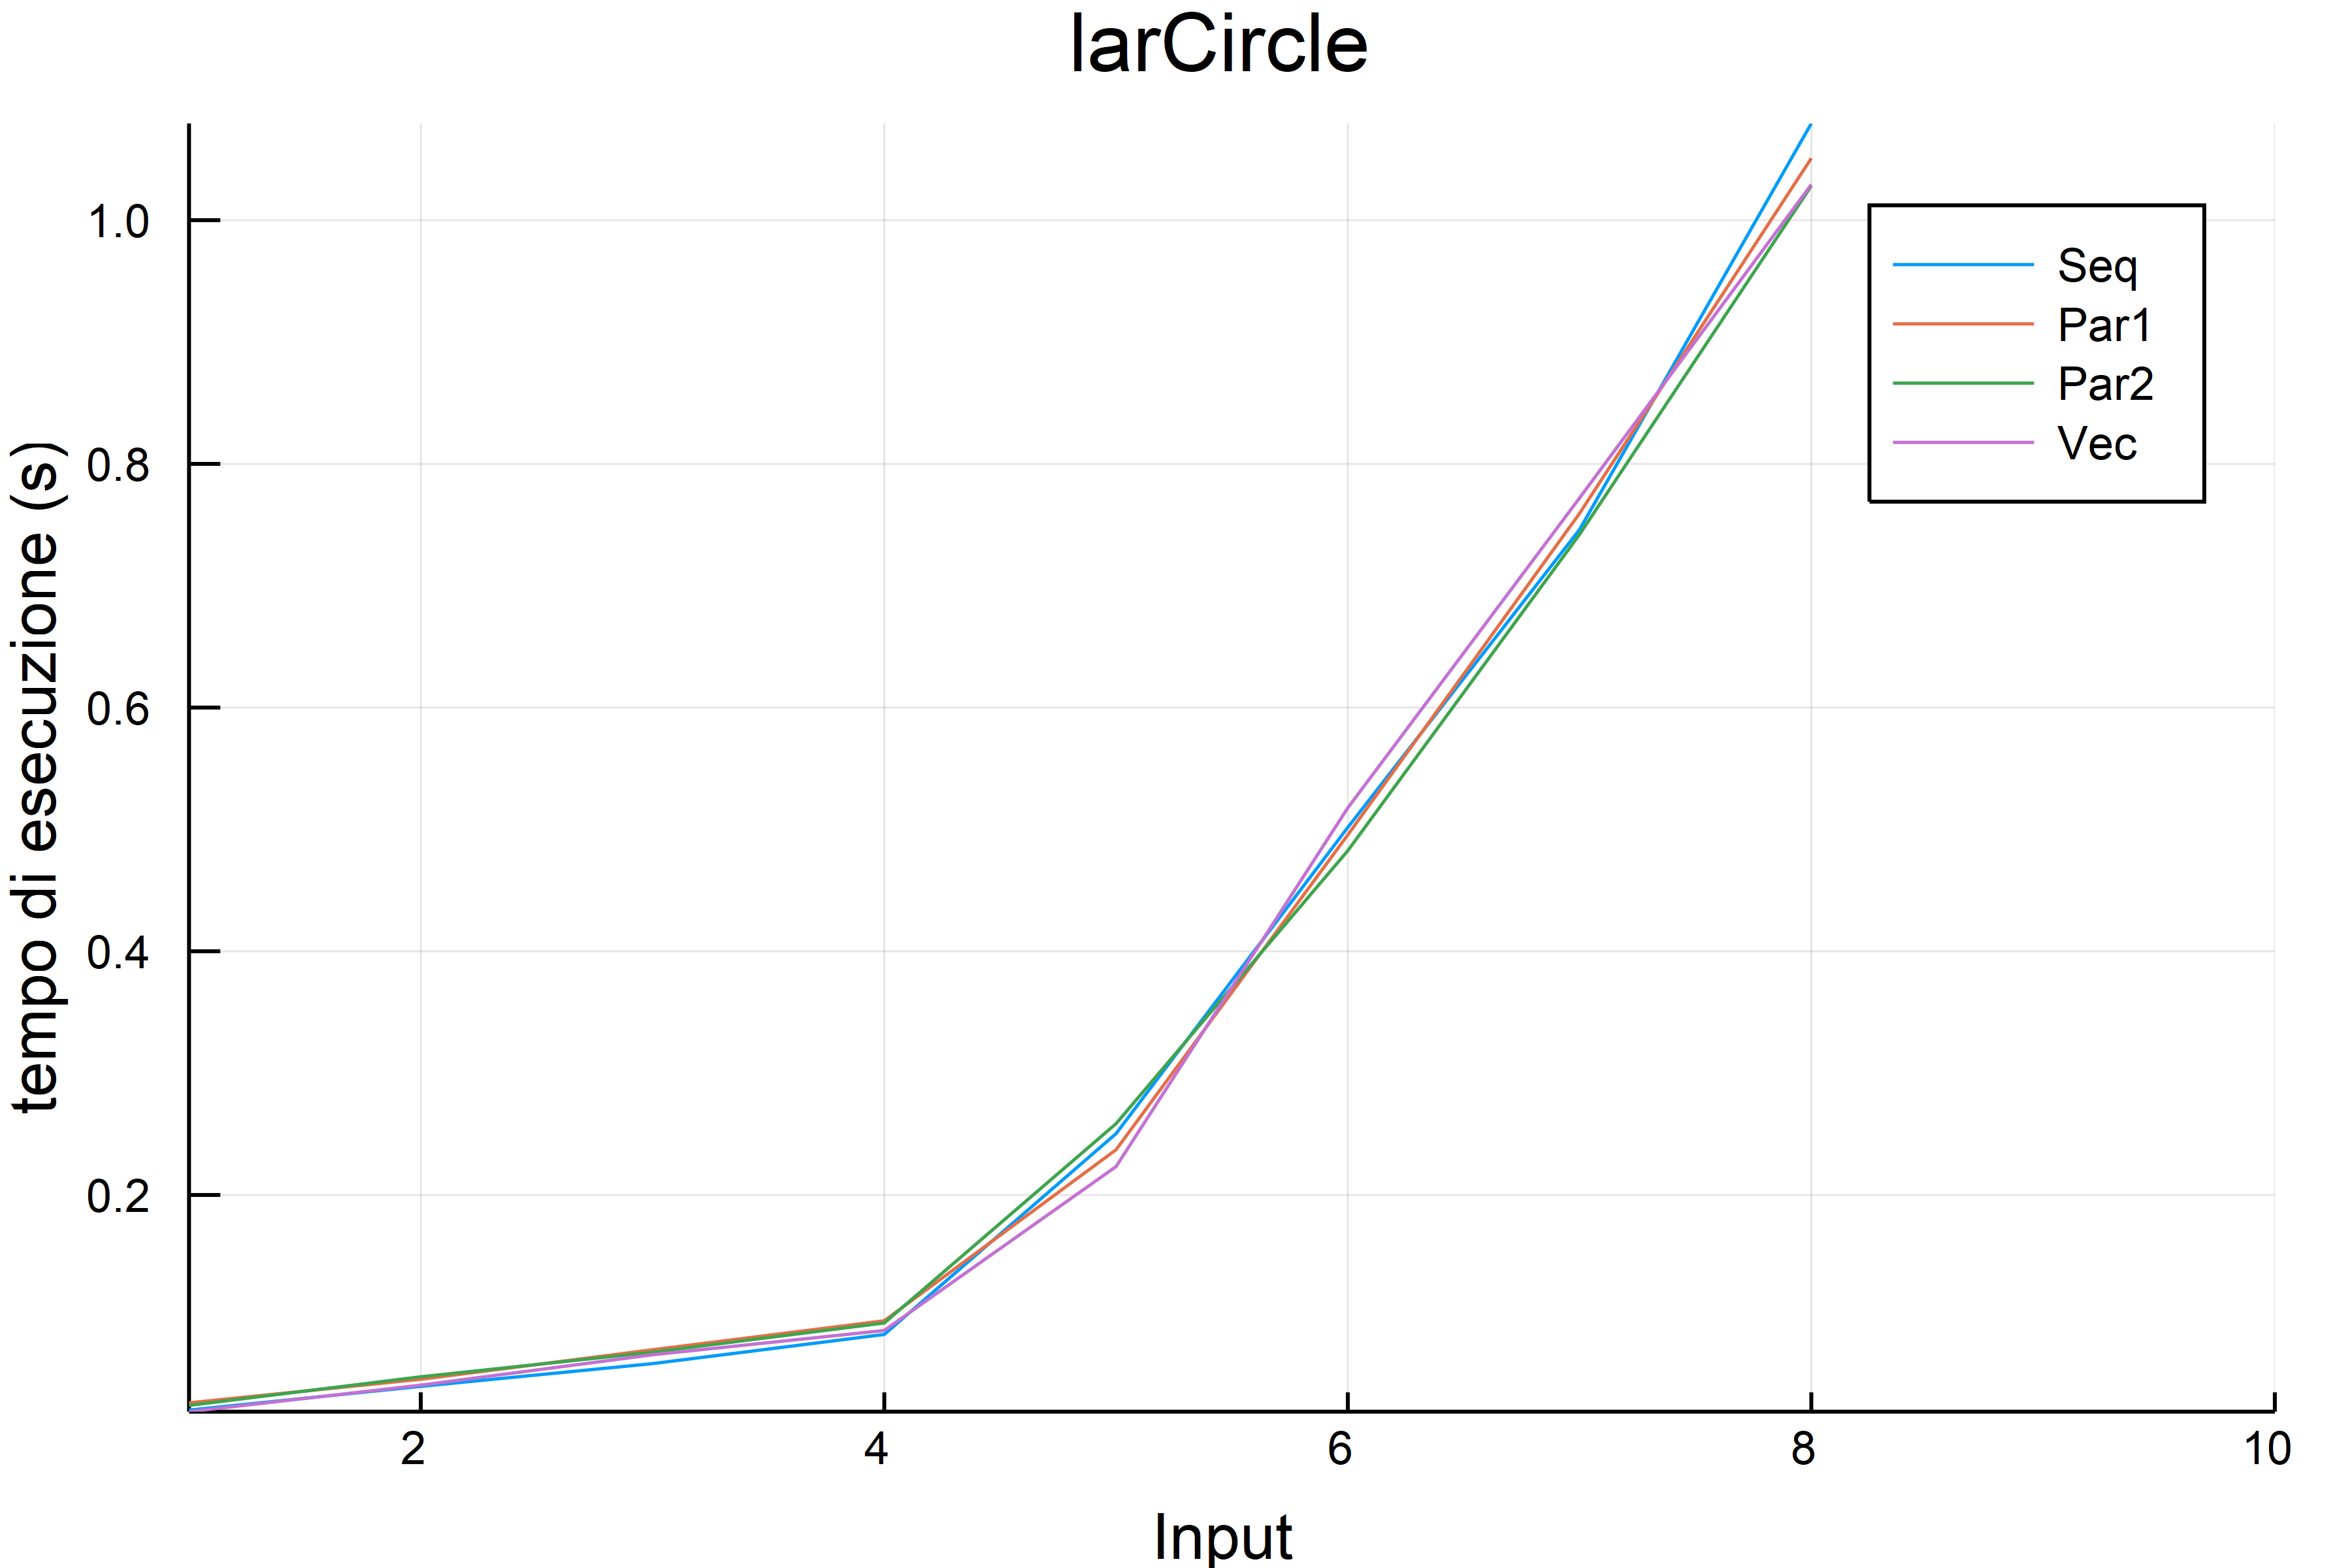
\includegraphics[scale=.13]{larCircleTime.png} 
\caption{Results computed on Microsoft Surface Pro  3 (4GB LPDDR3 1600 MHz RAM, i5-4300U processor)} 
\end{figure}

%---------------------------------------------------------------------------------
\subsection{larHelix}

\paragraph{Python}

\begin{verbatim}
def larHelix(radius=1.,pitch=1.,nturns=2,dim=1):
    def larHelix0(shape=36*nturns):
        angle = nturns*2*PI
        domain = larIntervals([shape])([angle])
        V,CV = domain
        x = lambda p : radius*COS(p[0])
        y = lambda p : radius*SIN(p[0])
        z = lambda p : (pitch/(2*PI)) * p[0]
        return larMap([x,y,z])(domain,dim)
    return larHelix0
\end{verbatim}

\paragraph{Julia}

\begin{verbatim}
function larHelix(radius=1.,pitch=1.,nturns=2)
    function larHelix0(shape=36*nturns)
        angle = nturns*2*pi
        V,CV = LARLIB.larCuboids([shape])
        V = (angle/shape)*V 
        W = hcat(map(u->[radius*cos(u);radius*sin(u);(pitch/(2*pi))*u],V)...)
        return W,CV
    end
    return larHelix0
end 
\end{verbatim}

The \textbf{larHelix} function creates an helix that wrap itself around the $z$ axis, with given radius, step and number of rounds.

Using the $larCuboids()$ function, contained in the LARLIB library, a domain shape is given in input and a cuboidal complex is created. This complex will be modified using the $map$ function to apply the desired parametrization to the coordinates of each vertex.

In this case, the local parametrization used is:
$$f(u)=(radius*cos(u),radius*sen(u),\tfrac{pitch}{2\pi}u),$$
dove $u \in [0,angle]$ e $angle=nturns*2*\pi$.

Then $map$ applies the "anonymous function"
$$\verb!u->[radius*cos(u);radius*sin(u);(pitch/(2*pi))*u]!$$ to the coordinates of all the vertices contained in the V collection.

Thus a new set of vertices is created; the coordinates are disposed vertically in a matrix using the $$\verb!hcat(A...)!$$ function.
\paragraph{Visualization examples}

\begin{verbatim}
V,CV = larHelix(1,0.5,4)()
V
CV
LARVIEW.viewexploded(V,CV)
\end{verbatim}

\begin{figure}[htbp] 
\centering 
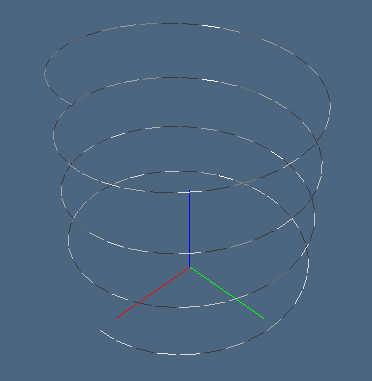
\includegraphics[scale=.43]{larHelix.png}
\caption{Unit radius helix on $z$ axis, with a step of 0.5 and 4 spins.} 
\end{figure}

\paragraph{Test}

\begin{Verbatim}
@testset "larHelix" begin
	@test BoxCalculation(larHelix()()[1])==8
	@test BoxCalculation(larHelix(2,2,2)()[1])==64
	@test BoxCalculation(larHelix(1,2,5)()[1])==40
	@test BoxCalculation(larHelix(1,1,3)()[1])==12
	#=
	radius=1, step=1, numspins=2, is contained
	in a box that has volume (radius*2)^2*step*numspins
	=#
	@test size(larHelix(5,7,9)()[1],2)==325
	@test length(larHelix(5,7,9)()[2])==324
end
\end{Verbatim}

\paragraph{Vectorization}

\begin{verbatim}
function larHelixV(radius=1.,pitch=1.,nturns=2)
    function larHelix0(shape=36*nturns)
        angle = nturns*2*pi
        V,CV = LARLIB.larCuboids([shape])
        W = (u->[radius*cos(u);radius*sin(u);
        (pitch/(2*pi))*u]).((x->x*angle/shape).(V))
        return hcat(W...),CV
    end
    return larHelix0
end 
\end{verbatim}

\paragraph{Parallel Computing} 

\begin{Verbatim}
function larHelixP(radius=1.,pitch=1.,nturns=2)
    function larHelix0(shape=36*nturns)
        angle = nturns*2*pi
        V,CV = LARLIB.larCuboids([shape])
        V = SharedArray(V)
        W = SharedArray{Float64}(3,size(V,2))
        @sync @parallel for i = 1:size(V,2)
            W[1,i] = radius*cos(V[i]*angle/shape)  
            W[2,i] = radius*sin(V[i]*angle/shape)
            W[3,i] = (pitch/(2*pi))*(V[i]*angle/shape)
        end
        return W,CV
    end
    return larHelix0
end
\end{Verbatim}

\begin{Verbatim}
@everywhere function flarHelix(SW::SharedArray,SV::Array,indexprt,ultim,
            shape,radius,pitch,nturns,angle)
    id = myid()
    if id != nprocs()
        for i=indexprt*(id-2) +1 : indexprt*(id-1)
            SW[1,i] = radius*cos(SV[i]*angle/shape)  
            SW[2,i] = radius*sin(SV[i]*angle/shape)
            SW[3,i] = (pitch/(2*pi))*(SV[i]*angle/shape)
        end
    else
        for i=indexprt*(id-2) +1 : ultim
            SW[1,i] = radius*cos(SV[i]*angle/shape)  
            SW[2,i] = radius*sin(SV[i]*angle/shape)
            SW[3,i] = (pitch/(2*pi))*(SV[i]*angle/shape)
        end
    end
end

function larHelixPP(radius=1.,pitch=1.,nturns=2)
    function larHelix0(shape=36*nturns)
        angle = nturns*2*pi
        V,CV = LARLIB.larCuboids([shape])
        W = SharedArray{Float64}(3,size(V,2))
        if nprocs() > size(V,2)
            indexprt = 1
        else
            indexprt = Int((size(V,2)-(size(V,2)%nprocs()))/nprocs())
        end
        @sync begin
            for i = 2:nprocs()
                @async remotecall_fetch(flarHelix,i,W,V,indexprt,size(V,2),
                shape,radius,pitch,nturns,angle)
            end
        end
        return W,CV 
    end
    return larHelix0 
end
\end{Verbatim}

\begin{Verbatim}
@testset "Vectorized and Parallelized larHelix" begin
    @test BoxCalculation(larHelixV()()[1])==8
    @test BoxCalculation(larHelixP(2,2,2)()[1])==64
    @test BoxCalculation(larHelixPP(1,2,5)()[1])==40
    @test BoxCalculation(larHelixP()()[1])==8
    @test BoxCalculation(larHelixPP(2,2,3)()[1])==96
    @test BoxCalculation(larHelixV(1,2,5)()[1])==40
end
\end{Verbatim}

\paragraph{Performance evaluation}

\begin{Verbatim}

x,y = TimeGraph(larHelix(),larHelixP(),larHelixPP(),larHelixV(),data1,5)
plot(x,y,yaxis=("tempo di esecuzione (s)"),xaxis=("Input",(1,length(x)+2)),
label=["Seq" "Par1" "Par2" "Vec"],title="larHelix",lw=1)

\end{Verbatim}

\begin{figure}[htbp] 
\centering 
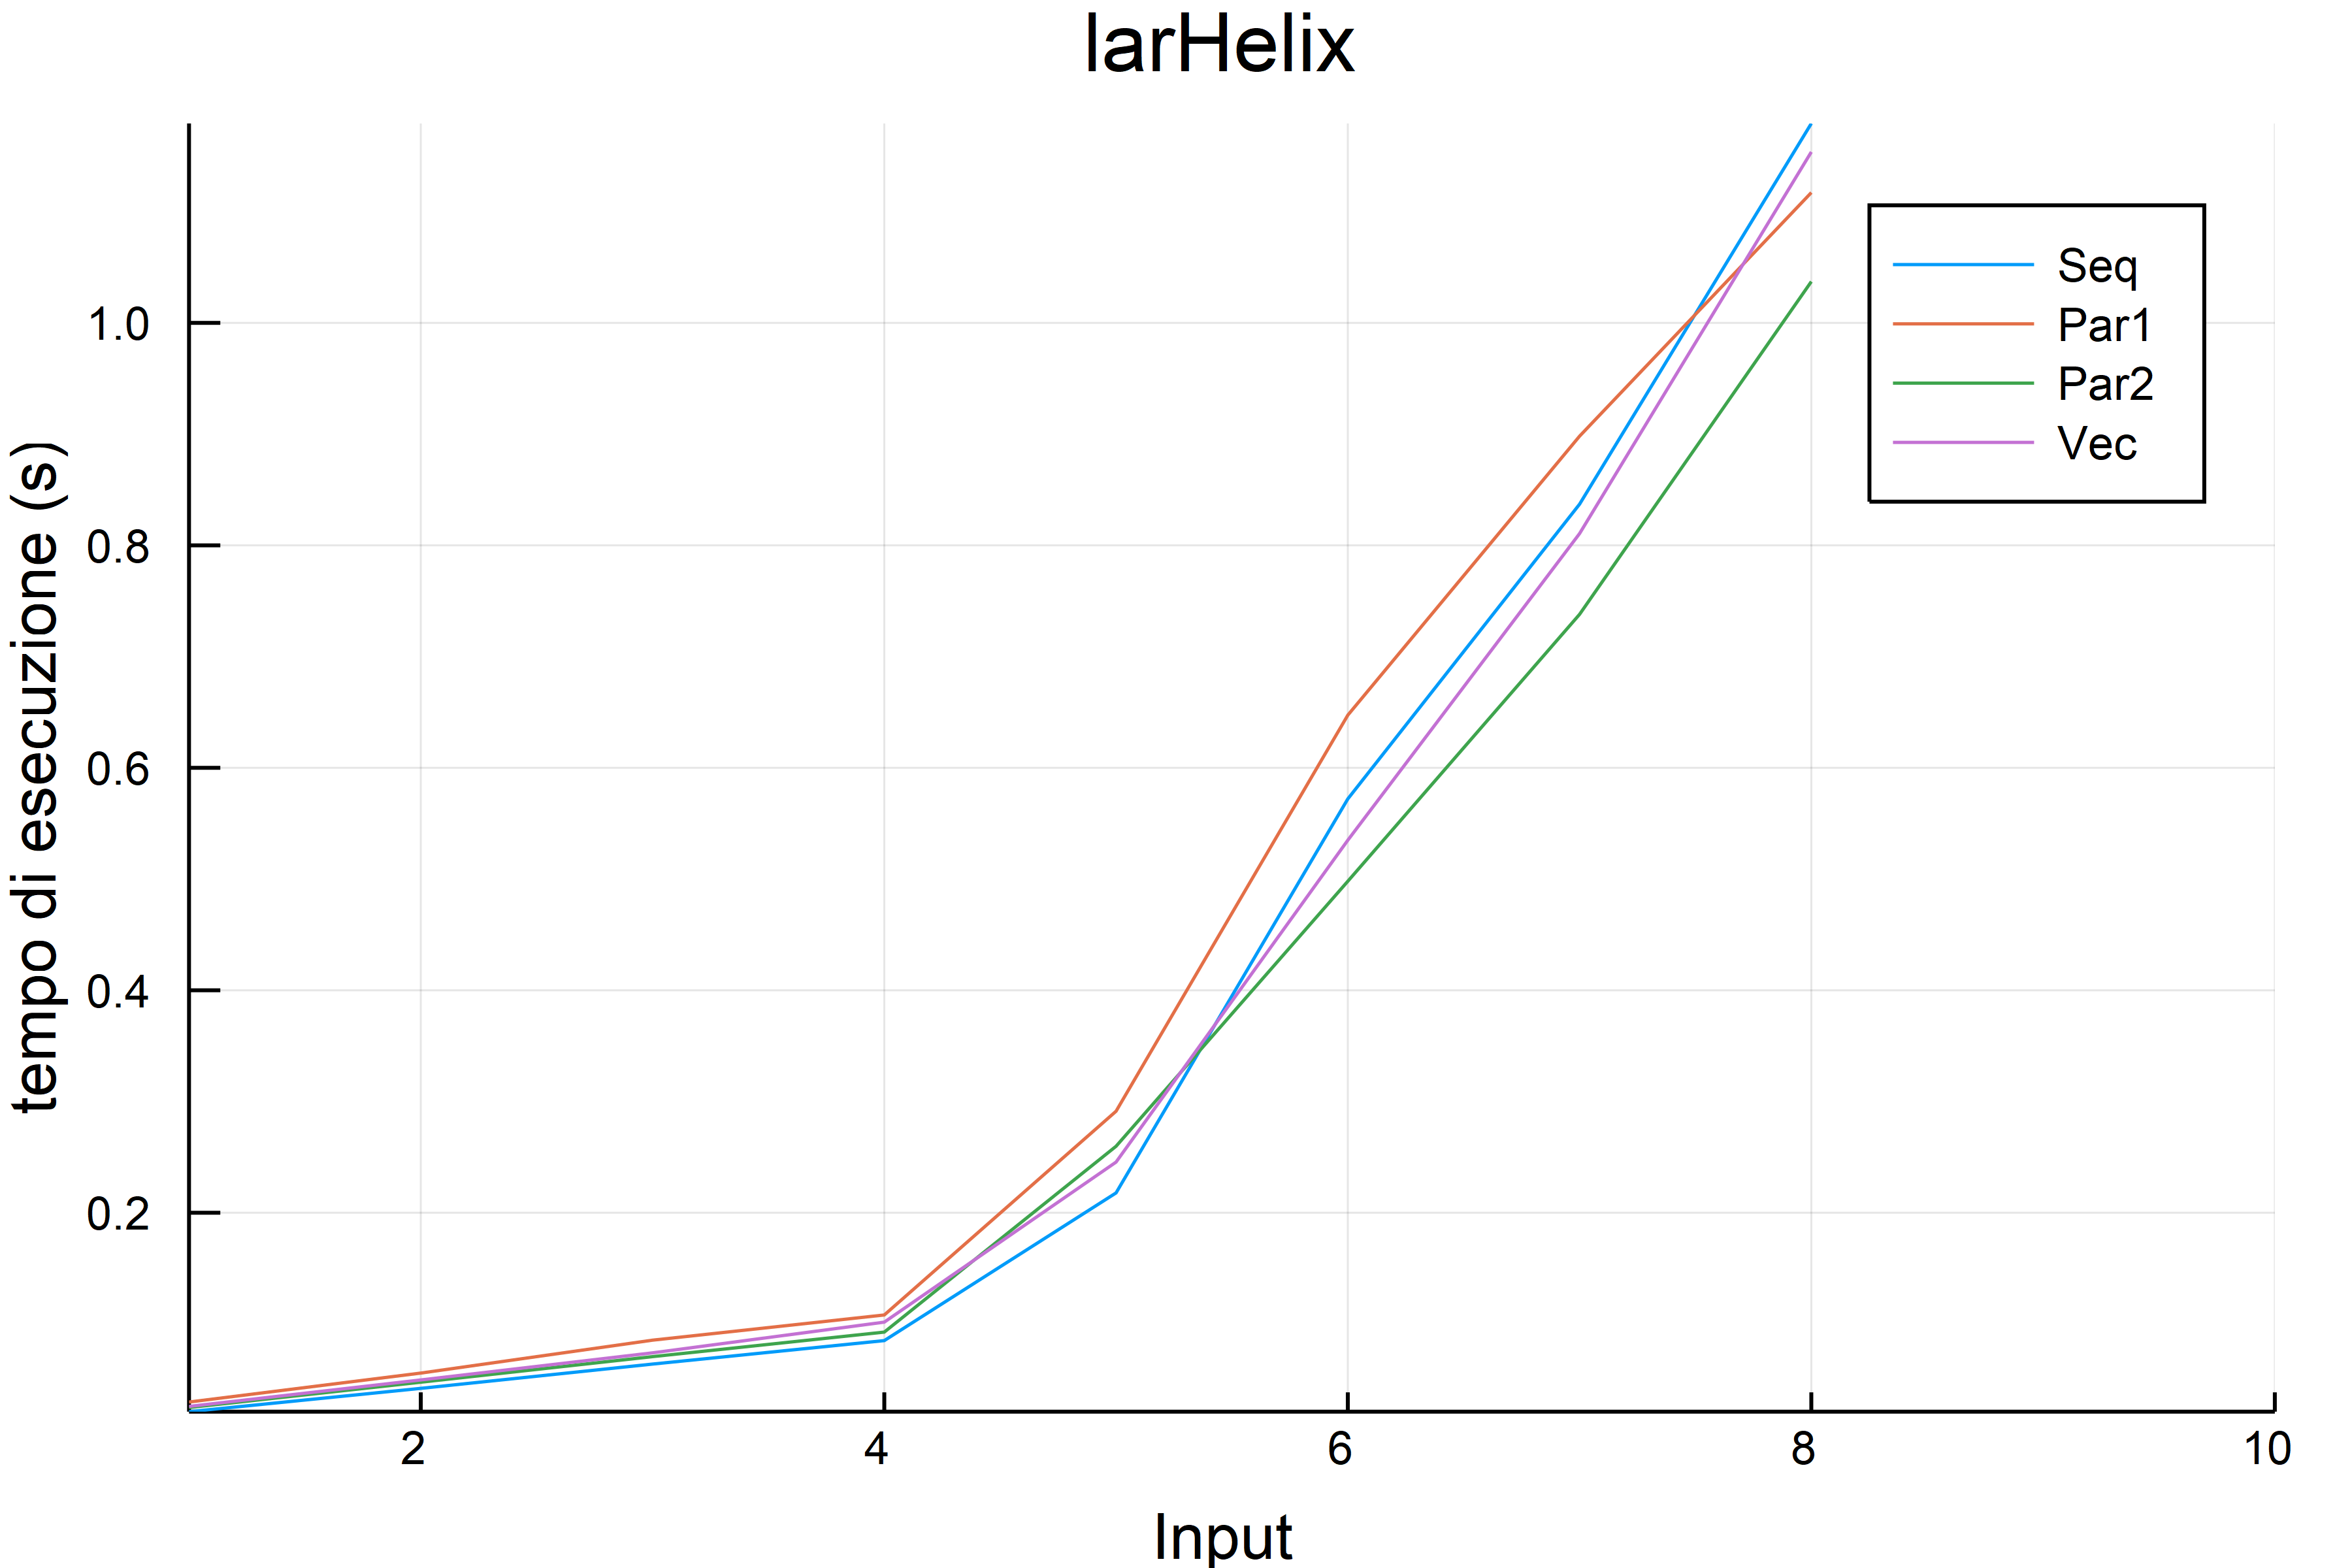
\includegraphics[scale=.13]{larHelixTime.png} 
\caption{Results computed on Microsoft Surface Pro  3 (4GB LPDDR3 1600 MHz RAM, i5-4300U processor)} 
\end{figure}


%---------------------------------------------------------------------------------
\subsection{larDisk}

\paragraph{Python}

\begin{verbatim}
def larDisk(radius=1.,angle=2*PI):
    def larDisk0(shape=[36,1]):
        domain = larIntervals(shape)([angle,radius])
        V,CV = domain
        x = lambda p : p[1]*COS(p[0])
        y = lambda p : p[1]*SIN(p[0])
        return larMap([x,y])(domain)
    return larDisk0
\end{verbatim}

\paragraph{Julia}
\begin{verbatim}
function larDisk(radius=1.,angle=2*pi)
    function larDisk0(shape=[36,1])
        V,CV = LARLIB.larCuboids(shape)
        V = [angle/shape[1] 0;0 radius/shape[2]]*V
        W = [V[:,k] for k=1:size(V,2)]
        Z = hcat(map(p->let(u,v)=p;[v*cos(u);v*sin(u)] end,W)...)
        return Z,CV
    end
    return larDisk0    
end
\end{verbatim}

The \textfb{larDisk} function creates a disk centered in the origin, with given radius and angle.

Using the $larCuboids()$ function, contained in the LARLIB library, a domain shape is given in input and a cuboidal complex is created. This complex will be modified using the $map$ function to apply the desired parametrization to the coordinates of each vertex.

In this case, the local parametrization used is: $$f(u,v)=(vcos(u),vsen(u)),$$
with $[u,v] \in [0,angle]\times[0,radius]$.

Then $map$ applies the "anonymous function"
$$\verb!p->let(u,v)=p;[v*cos(u);v*sin(u)] end!$$ to the coordinates of all the vertices contained in the V collection.

Thus a new set of vertices is created; the coordinates are disposed vertically in a matrix using the $$\verb!hcat(A...)!$$ function.

\paragraph{Visualization examples}

\begin{verbatim}
V,CV = larDisk()([36,4])
V
CV
LARVIEW.viewexploded(V,CV)
\end{verbatim}

\begin{figure}[htbp] 
\centering 
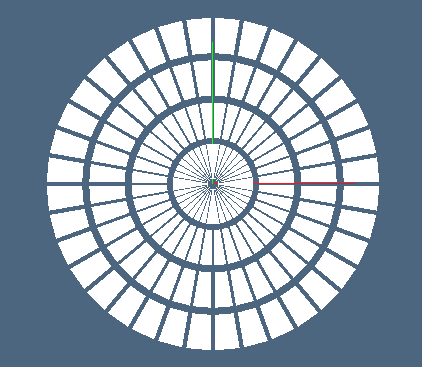
\includegraphics[scale=.45]{larDisk.png} 
\caption{Unit radius disk centered in the origin.} 
\end{figure}

\paragraph{Test}

\begin{Verbatim}
@testset "larDisk" begin
	@test BoxCalculation(larDisk()()[1])==4
	@test BoxCalculation(larDisk(2,2*pi)()[1])==16
	@test BoxCalculation(larDisk(3,pi)()[1])==18
	@test BoxCalculation(larDisk(5,pi/2)()[1])==25
	#(radius*2)^2
	@test size(larDisk(10,pi/7)()[1],2)==74
	@test length(larDisk(10,pi/7)()[2])==36
end
\end{Verbatim}

\paragraph{Vectorization}

\begin{verbatim}
function larDiskV(radius=1.,angle=2*pi)
    function larDisk0(shape=[36,1])
        V,CV = LARLIB.larCuboids(shape)
        V = [V[:,k] for k=1:size(V,2)]
        W = (p->[p[2]*cos(p[1]);p[2]*sin(p[1])]).((p->[p[1]*angle/shape[1], p[2]*radius/shape[2]]).(V))
        return hcat(W...),CV
    end
    return larDisk0    
end
\end{verbatim}

\paragraph{Parallel Computing} 

\begin{Verbatim}
function larDiskP(radius=1.,angle=2*pi)
    function larDisk0(shape=[36,1])
        V,CV = LARLIB.larCuboids(shape)
        V = SharedArray(V)
        W = SharedArray{Float64}(2,size(V,2))
        @sync @parallel for i = 1:size(V,2)
            W[1,i] = (V[2,i]*radius/shape[2])*cos(V[1,i]*angle/shape[1])
            W[2,i] = (V[2,i]*radius/shape[2])*sin(V[1,i]*angle/shape[1])
        end
        return W,CV
    end
    return larDisk0    
end
\end{Verbatim}

\begin{Verbatim}
@everywhere function flarDisk(W::SharedArray,V::Array,indexprt,ultim,
            shape,radius,angle)
    id = myid()
    if id != nprocs()
        for i=indexprt*(id-2) +1 : indexprt*(id-1)
            W[1,i] = (V[2,i]*radius/shape[2])*cos(V[1,i]*angle/shape[1])
            W[2,i] = (V[2,i]*radius/shape[2])*sin(V[1,i]*angle/shape[1])  
        end
    else
        for i=indexprt*(id-2) +1 : ultim
            W[1,i] = (V[2,i]*radius/shape[2])*cos(V[1,i]*angle/shape[1])
            W[2,i] = (V[2,i]*radius/shape[2])*sin(V[1,i]*angle/shape[1])
        end
    end
end

function larDiskPP(radius=1.,angle=2*pi)
    function larDisk0(shape=[36,1])
        V,CV = LARLIB.larCuboids(shape)
        W = SharedArray{Float64}(2,size(V,2))
        if nprocs() > size(V,2)
            indexprt = 1
        else
            indexprt = Int((size(V,2)-(size(V,2)%nprocs()))/nprocs())
        end
        @sync begin
            for i = 2:nprocs()
                @async remotecall_fetch(flarDisk,i,W,V,indexprt,size(V,2),
                shape,radius,angle)
            end
        end
        return W,CV
    end
    return larDisk0    
end
\end{Verbatim}

\begin{Verbatim}
@testset "Vectorized and Parallelized larDisk" begin
    @test BoxCalculation(larDiskV()([56,1])[1])==4
    @test BoxCalculation(larDiskP(2,2*pi)([56,1])[1])==16
    @test BoxCalculation(larDiskPP(3,pi)([56,1])[1])==18
    @test BoxCalculation(larDiskP()([56,1])[1])==4
    @test BoxCalculation(larDiskPP(2,2*pi)([56,1])[1])==16
    @test BoxCalculation(larDiskV(3,pi)([56,1])[1])==18 
end
\end{Verbatim}

\paragraph{Performance evaluation}

\begin{Verbatim}
data = [[n,1] for n in data2]

x,y = TimeGraph(larDisk(),larDiskP(),larDiskPP(),larDiskV(),data,5)
plot(x,y,yaxis=("tempo di esecuzione (s)"),xaxis=("Input",(1,length(x)+2)),
label=["Seq" "Par1" "Par2" "Vec"],title="larDisk",lw=1)

\end{Verbatim}

\begin{figure}[htbp] 
\centering 
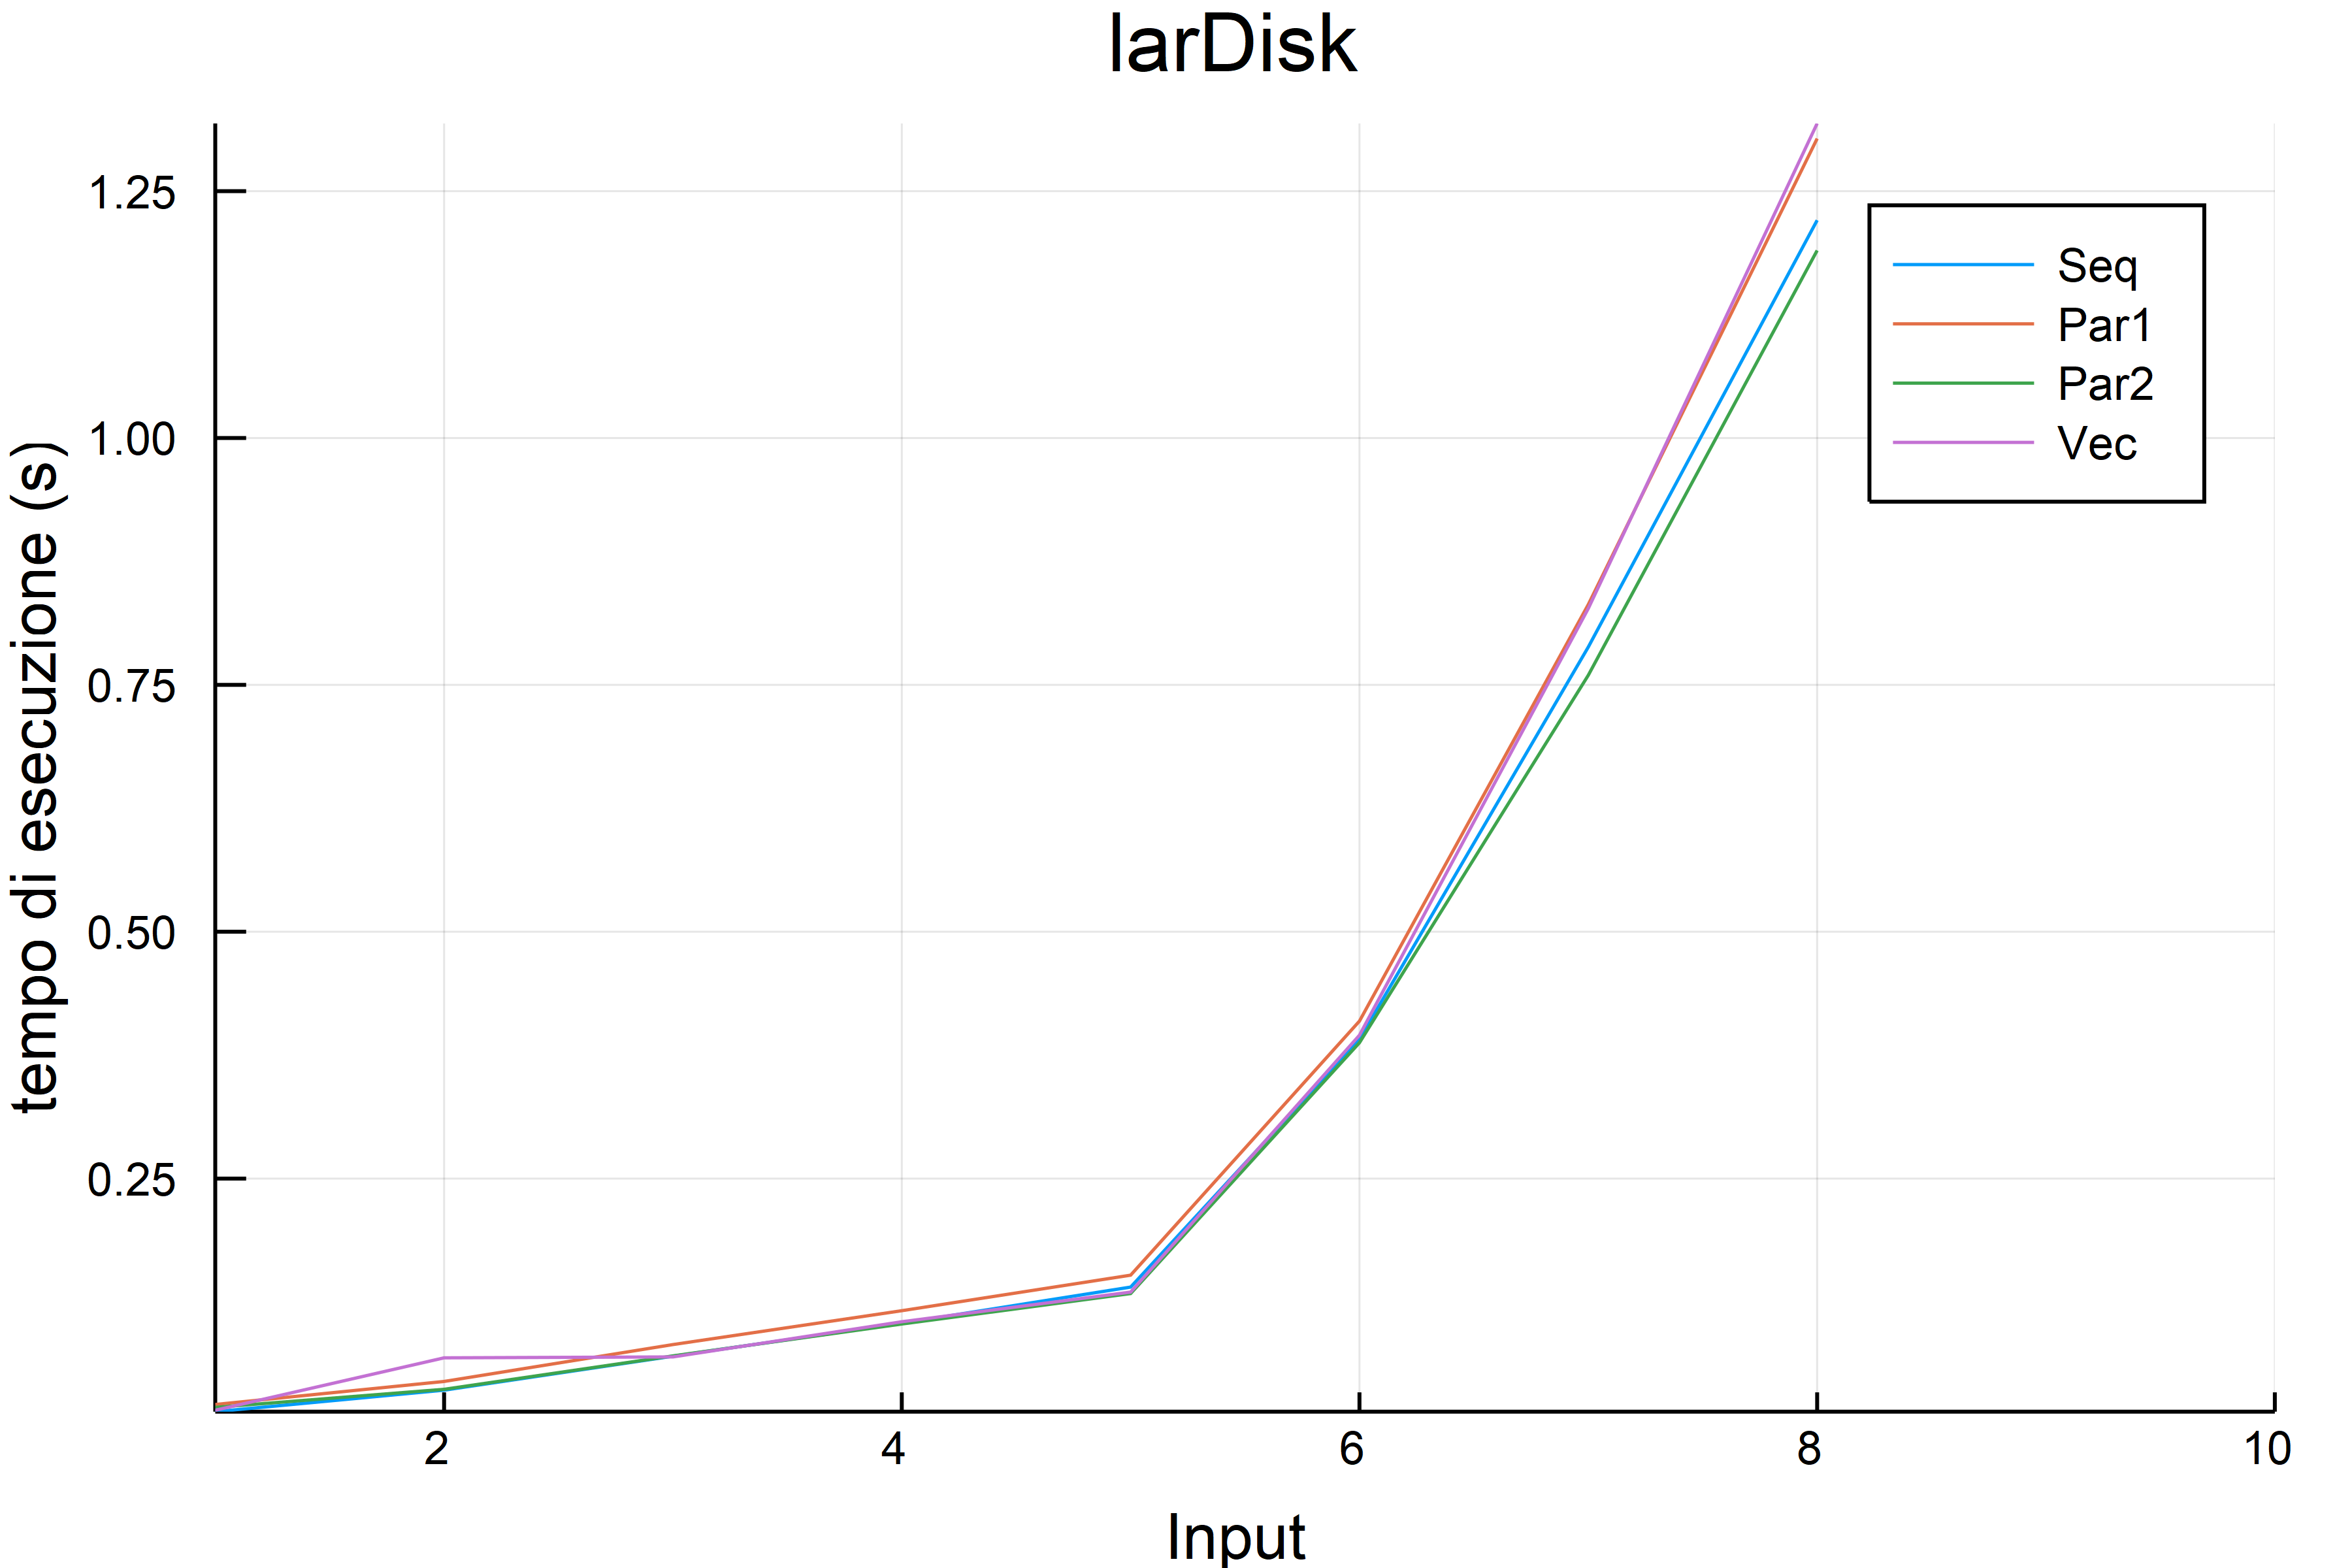
\includegraphics[scale=.13]{larDiskTime.png} 
\caption{Results computed on Microsoft Surface Pro  3 (4GB LPDDR3 1600 MHz RAM, i5-4300U processor)} 
\end{figure}

%---------------------------------------------------------------------------------
\subsection{larHelicoid}

\paragraph{Python}

\begin{verbatim}
def larHelicoid(R=1.,r=0.5,pitch=1.,nturns=2,dim=1):
    def larHelicoid0(shape=[36*nturns,2]):
        angle = nturns*2*PI
        domain = larIntervals(shape,'simplex')([angle,R-r])
        V,CV = domain
        V = larTranslate([0,r,0])(V)
        domain = V,CV
        x = lambda p : p[1]*COS(p[0])
        y = lambda p : p[1]*SIN(p[0])
        z = lambda p : (pitch/(2*PI)) * p[0]
        return larMap([x,y,z])(domain,dim)
    return larHelicoid0
\end{verbatim}

\paragraph{Julia}

\begin{verbatim}
function larHelicoid(R=1.,r=0.5,pitch=1.,nturns=2)
    function larHelicoid0(shape=[36*nturns,2])
        angle = nturns*2*pi
        V,CV = larSimplexGrid1(shape)
        V = [angle/shape[1] 0;0 (R-r)/shape[2]]*V
        V = broadcast(+,V,[0,r])
        W = [V[:,k] for k=1:size(V,2)]
        X = hcat(map(p->let(u,v)=p;[v*cos(u);v*sin(u);
        	(pitch/(2*pi))*u] end,W)...)
        return X,CV
    end
    return larHelicoid0    
end
\end{verbatim}

The \textfb{larHelicoid} function creates an helical surface that wrap itself around the $z$ axis, with given radius, step and number of rounds.

Using the $larCuboids()$ function, contained in the LARLIB library, a domain shape is given in input and a cuboidal complex is created. This complex will be modified using the $map$ function to apply the desired parametrization to the coordinates of each vertex.

In this case, the local parametrization used is:
$$f(u,v)=(v*cos(u),v*sen(u),\tfrac{pitch}{2\pi}u),$$
with $[u,v] \in [0,angle]\times[r,R]$.

With $$\verb!V=broadcast(+,V,[0,r])!$$ we sum 0 to every element in the first row of V and $r$ to every element in the second row of V.

With $$\verb!W=[V[:,k] for k=1:size(V,2)]!,$$ as opposed to $hcat$, we dispose the coordinates of the vertices (i.e. the columns in V) horizontally (into an array of arrays).

Then $map$ applies the "anonymous function" $$\verb!p->let(u,v)=p;[v*cos(u);v*sin(u);(pitch/(2*pi))*u] end!$$ to the coordinates of all the vertices contained in the W collection.

Thus a new set of vertices is created; the coordinates are disposed vertically in a matrix using the $$\verb!hcat(A...)!$$ function.

\paragraph{Visualization examples}

\begin{verbatim}
V,CV = larHelicoid()()
V
CV
W = [Any[V[h,k] for h=1:size(V,1)] for k=1:size(V,2)]
hpc = p.STRUCT(p.MKPOLS(PyObject([W,CV,[]])))
p.VIEW(hpc)
\end{verbatim}

\begin{figure}[htbp] 
\centering 
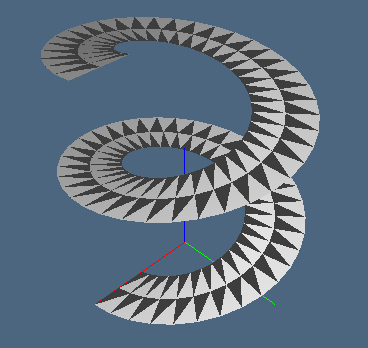
\includegraphics[scale=.5]{larHelicoid.png} 
\caption{Helical surface on the $z$ axis with radius of 0.5 and 1, step of 0.5 and 2 spins.} 
\end{figure}

\paragraph{Test}

\begin{Verbatim}
@testset "larHelicoid" begin
	@test BoxCalculation(larHelicoid()()[1])==8
	@test BoxCalculation(larHelicoid(2,1,2,2)()[1])==64
	@test BoxCalculation(larHelicoid(1,0.5,2,5)()[1])==40
	@test BoxCalculation(larHelicoid(1,0.3,1,3)()[1])==12
	#=
	raggio=1, passo=1, numgiri=2, è contenuto in un
	parallelepipedo di volume (raggio*2)^2*passo*numgiri
	=#
	@test size(larHelicoid(1.3,0.7,1,3)()[1],2)==327
	@test length(larHelicoid(1.3,0.7,1,3)()[2])==432
end
\end{Verbatim}

\paragraph{Vectorization}
\begin{Verbatim}
function larHelicoidV(R=1.,r=0.5,pitch=1.,nturns=2)
    function larHelicoid0(shape=[36*nturns,2])
        angle = nturns*2*pi
        V,CV = larSimplexGrid1(shape)
        V = [V[:,k] for k=1:size(V,2)]
        W = (p->[p[2]*cos(p[1]);p[2]*sin(p[1]);
            (pitch/(2*pi))*p[1]]).((x->[x[1]*angle/shape[1], x[2]*(R-r)/shape[2]+r]).(V))
        return hcat(W...),CV
    end
    return larHelicoid0    
end
\end{Verbatim}

\paragraph{Parallel Computing} 

\begin{Verbatim}
function larHelicoidP(R=1.,r=0.5,pitch=1.,nturns=2)
    function larHelicoid0(shape=[36*nturns,2])
        angle = nturns*2*pi
        V,CV = larSimplexGrid1(shape)
        V = SharedArray(V)
        W = SharedArray{Float64}(3,size(V,2))
        @sync @parallel for i = 1:size(V,2)
            W[1,i] = (V[2,i]*(R-r)/shape[2]+r) *cos(V[1,i]*angle/shape[1])
            W[2,i] = (V[2,i]*(R-r)/shape[2]+r) *sin(V[1,i]*angle/shape[1])
            W[3,i] = (pitch/(2*pi))*(V[1,i]*angle/shape[1])
        end
        return W,CV
    end
    return larHelicoid0    
end
\end{Verbatim}

\begin{Verbatim}
@everywhere function flarHelicoid(W::SharedArray,V::Array,indexprt,ultim,
            shape,R,r,pitch,nturns,angle)
    id = myid()
    if id != nprocs()
        for i=indexprt*(id-2) +1 : indexprt*(id-1)
            W[1,i] = (V[2,i]*(R-r)/shape[2]+r) *cos(V[1,i]*angle/shape[1])
            W[2,i] = (V[2,i]*(R-r)/shape[2]+r) *sin(V[1,i]*angle/shape[1])
            W[3,i] = (pitch/(2*pi))*(V[1,i]*angle/shape[1]) 
        end
    else
        for i=indexprt*(id-2) +1 : ultim
            W[1,i] = (V[2,i]*(R-r)/shape[2]+r) *cos(V[1,i]*angle/shape[1])
            W[2,i] = (V[2,i]*(R-r)/shape[2]+r) *sin(V[1,i]*angle/shape[1])
            W[3,i] = (pitch/(2*pi))*(V[1,i]*angle/shape[1])
        end
    end
end


function larHelicoidPP(R=1.,r=0.5,pitch=1.,nturns=2)
    function larHelicoid0(shape=[36*nturns,2])
        angle = nturns*2*pi
        V,CV = larSimplexGrid1(shape)
        W = SharedArray{Float64}(3,size(V,2))
        if nprocs() > size(V,2)
            indexprt = 1
        else
            indexprt = Int((size(V,2)-(size(V,2)%nprocs()))/nprocs())
        end
        @sync begin
            for i = 2:nprocs()
                @async remotecall_fetch(flarHelicoid,i,W,V,indexprt,size(V,2),
                shape,R,r,pitch,nturns,angle)
            end
        end
        return W,CV
    end
    return larHelicoid0    
end
\end{Verbatim}

\begin{Verbatim}
@testset "Vectorized and Parallelized larHelicoid" begin
    @test BoxCalculation(larHelicoidV()()[1])==8
    @test BoxCalculation(larHelicoidP(2,1,2,2)()[1])==64
    @test BoxCalculation(larHelicoidPP(1,0.5,2,5)()[1])==40
    @test BoxCalculation(larHelicoidP()()[1])==8
    @test BoxCalculation(larHelicoidPP(2,1,2,2)()[1])==64
    @test BoxCalculation(larHelicoidV(1,0.5,2,5)()[1])==40
end
\end{Verbatim}

\paragraph{Performance evaluation}

\begin{Verbatim}
data = [[n,1] for n in data3]

x,y = TimeGraph(larHelicoid(),larHelicoidP(),larHelicoidPP(),larHelicoidV(),data,5)
plot(x,y,yaxis=("tempo di esecuzione (s)"),xaxis=("Input",(1,length(x)+2)),
label=["Seq" "Par1" "Par2" "Vec"],title="larHelicoid",lw=1)

\end{Verbatim}

\begin{figure}[htbp] 
\centering 
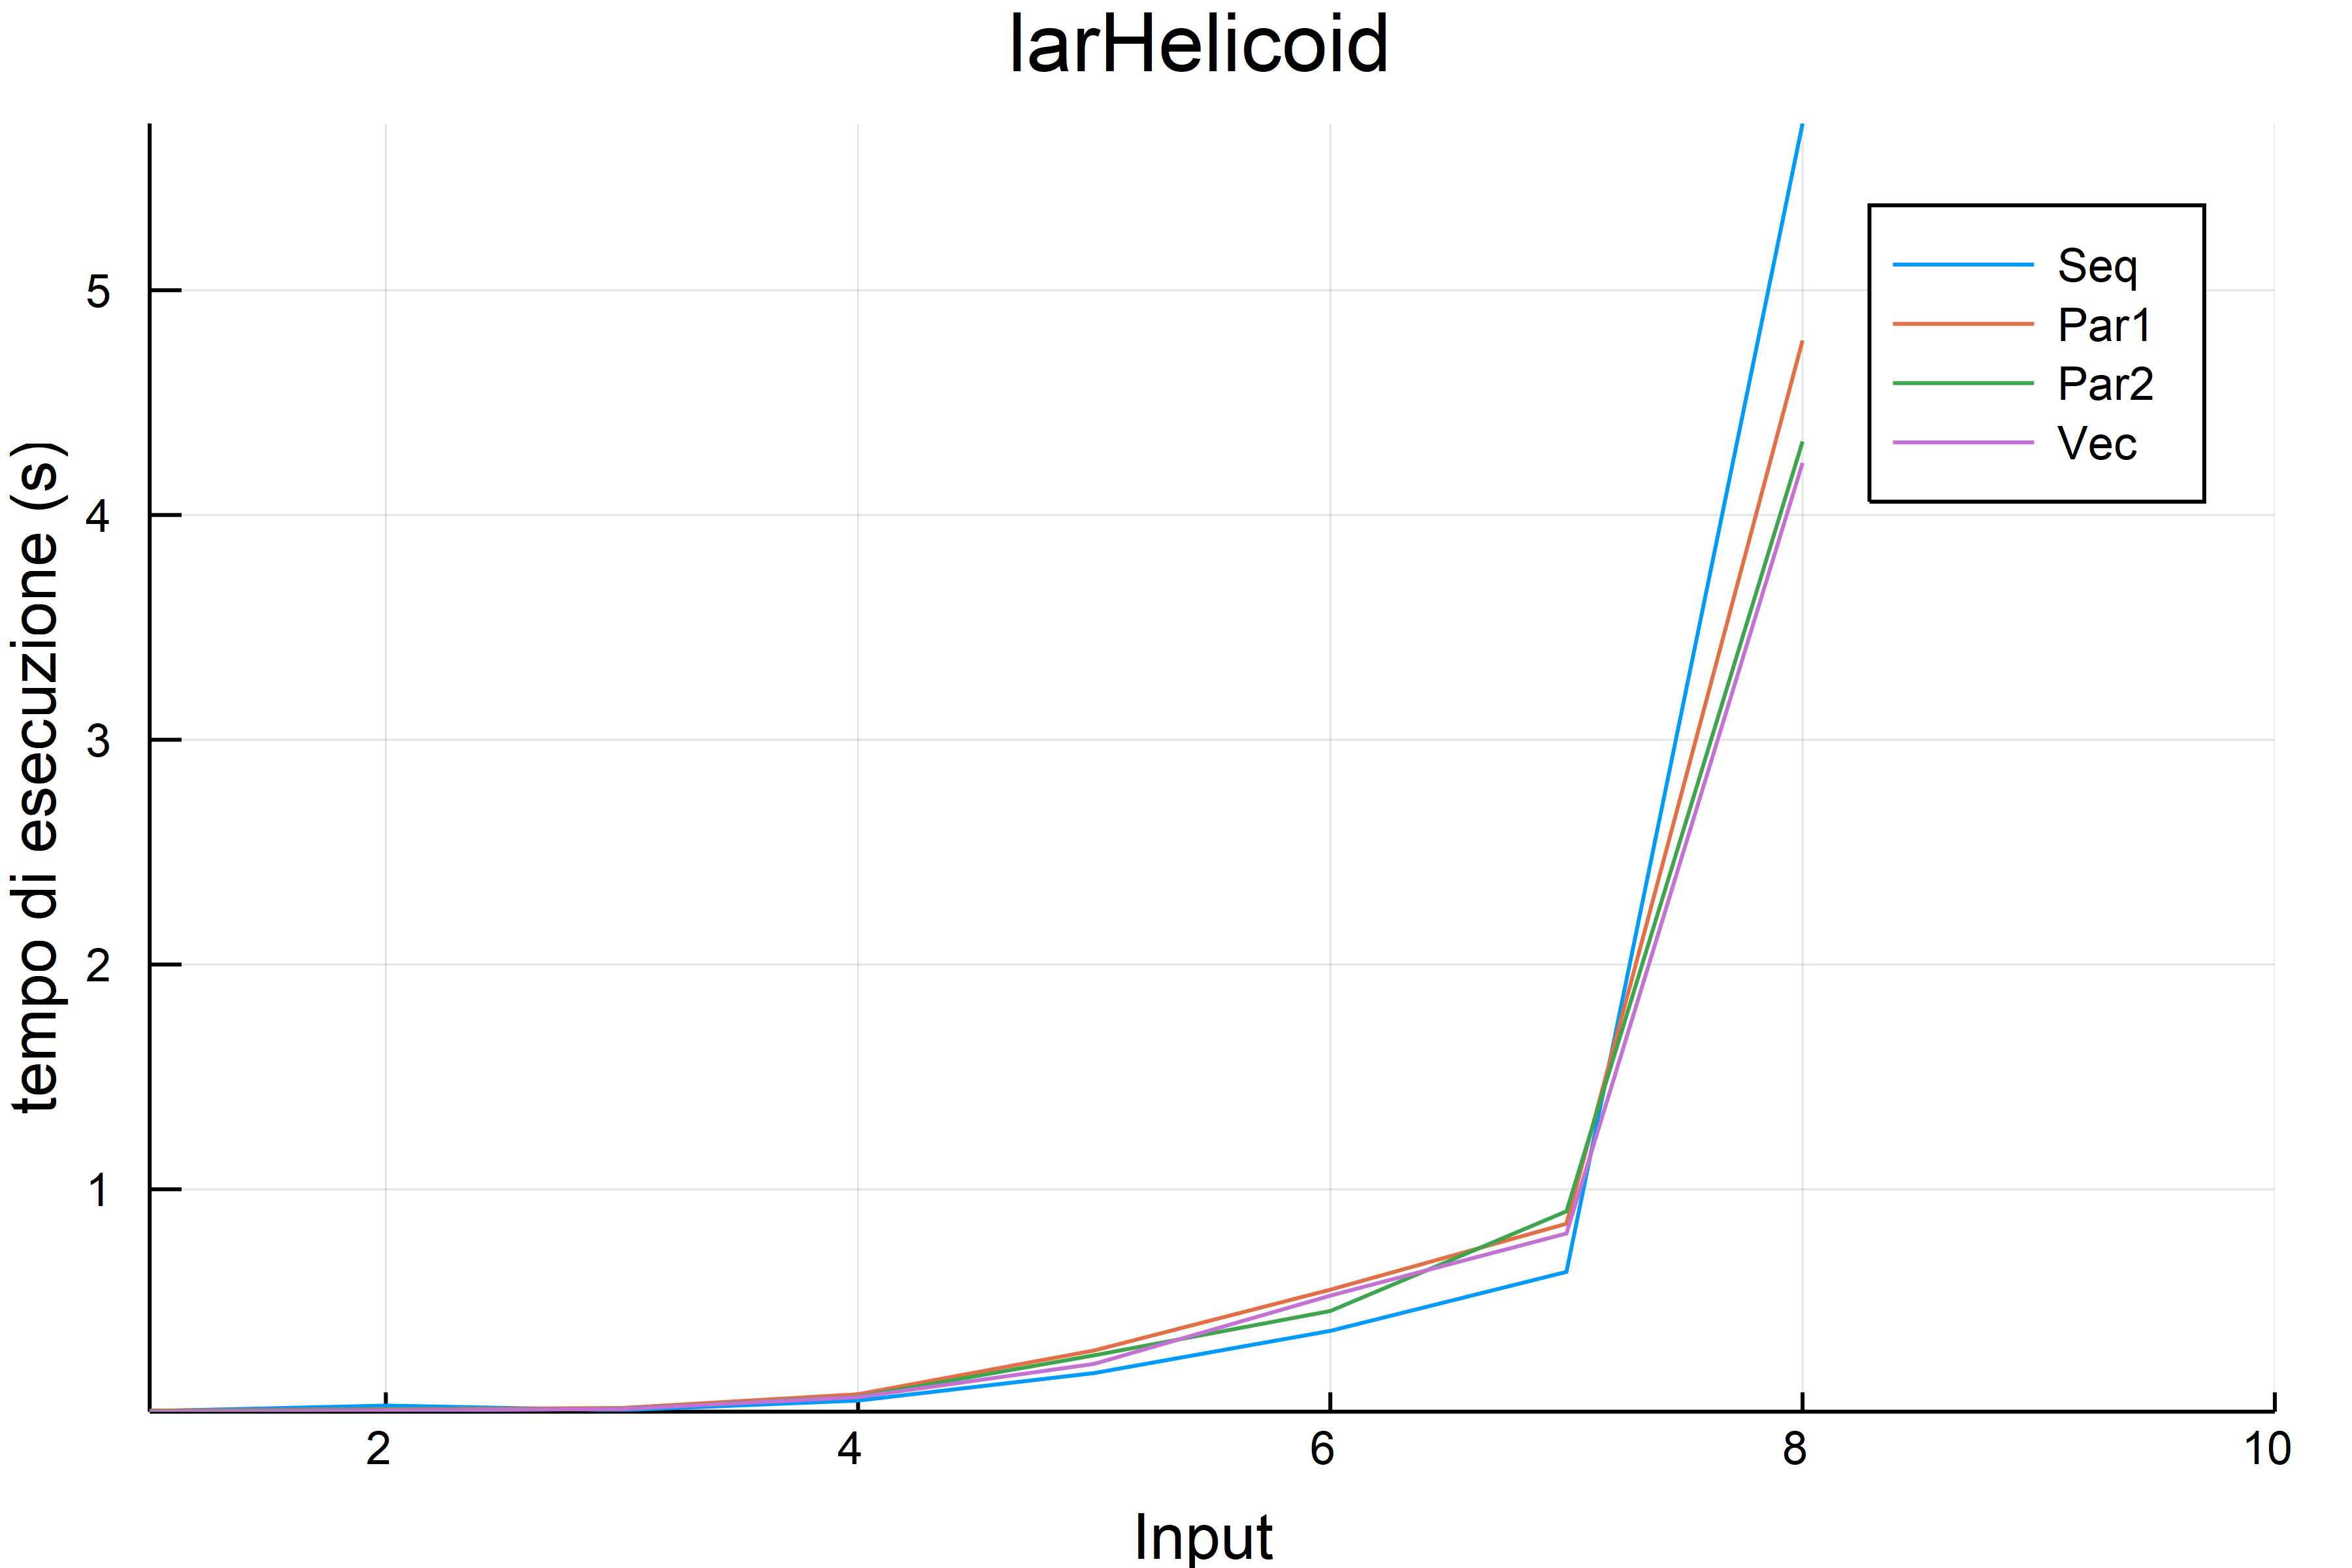
\includegraphics[scale=.13]{larHelicoidTime.png} 
\caption{Results computed on Microsoft Surface Pro  3 (4GB LPDDR3 1600 MHz RAM, i5-4300U processor)} 
\end{figure}
%---------------------------------------------------------------------------------
\subsection{larRing}

\paragraph{Python}

\begin{verbatim}
def larRing(r1,r2,angle=2*PI):
    def larRing0(shape=[36,1]):
        V,CV = larIntervals(shape)([angle,r2-r1])
        V = larTranslate([0,r1])(V)
        domain = V,CV
        x = lambda p : p[1] *  COS(p[0])
        y = lambda p : p[1] * SIN(p[0])
        return larMap([x,y])(domain)
    return larRing0	
\end{verbatim}

\paragraph{Julia}

\begin{verbatim}
function larRing(r1,r2,angle=2*pi)
    function larRing0(shape=[36,1])
        V,CV = LARLIB.larCuboids(shape)
        V = [angle/shape[1] 0;0 (r2-r1)/shape[2]]*V
        V = broadcast(+,V,[0,r1])
        W = [V[:,k] for k=1:size(V,2)]
        Z = hcat(map(p->let(u,v)=p;[v*cos(u);v*sin(u)] end,W)...)
        return Z,CV
    end
    return larRing0
end
\end{verbatim}

The \textfb{larRing} function creates a ring centered in the origin with given radiuses and angle.

In this case, the local parametrization used is:
$$f(u,v)=(vcos(u),vsen(u)),$$
with $[u,v] \in [0,angle]\times[r1,r2]$.

With $$\verb!V=broadcast(+,V,[0,r1])!$$ we sum 0 to every element in the first row of V and $r1$ to every element in the second row of V.

With $$\verb!W=[V[:,k] for k=1:size(V,2)]!,$$ as opposed to $hcat$, we dispose the coordinates of the vertices (i.e. the columns in V) horizontally (into an array of arrays).

Then $map$ applies the "anonymous function" $$\verb!p->let(u,v)=p;[v*cos(u);v*sin(u)] end!$$ to the coordinates of all the vertices contained in the W collection.

Thus a new set of vertices is created; the coordinates are disposed vertically in a matrix using the $$\verb!hcat(A...)!$$ function.

\paragraph{Visualization examples}

\begin{verbatim}
V,CV = larRing(1,3,2*pi)([36,1])
V
CV
LARVIEW.viewexploded(V,CV)
\end{verbatim}
\begin{figure}[htbp] 
\centering 
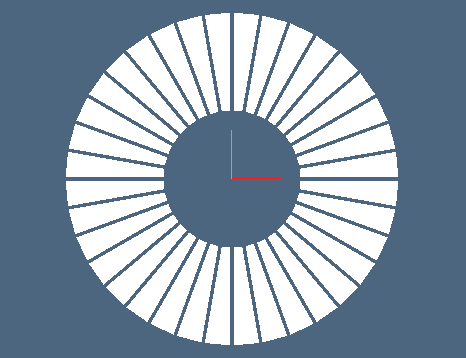
\includegraphics[scale=.4]{larRing.png} 
\caption{Ring centered in the origin of radiuses 1 and 3.} 
\end{figure}

\begin{verbatim}
V,CV = larRing(3,7,pi)([80,10])
LARVIEW.viewexploded(V,CV)
\end{verbatim}
\begin{figure}[htbp] 
\centering 
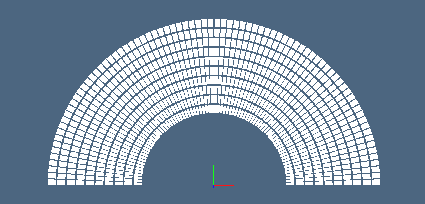
\includegraphics[scale=.5]{larRing2.png} 
\caption{Half ring centered in the origin of radiuses 3 and 7.} 
\end{figure}

\paragraph{Test}

\begin{Verbatim}
@testset "larRing" begin
	@test BoxCalculation(larRing(1,3,2*pi)()[1])==36
	@test BoxCalculation(larRing(1,2,pi)()[1])==8
	@test BoxCalculation(larRing(2,5,pi/2)()[1])==25
	#(radius*2)^2
	@test size(larRing(5,10,pi/6)()[1],2)==74
	@test length(larRing(5,10,pi/6)()[2])==36
end
\end{Verbatim}

\paragraph{Vectorization}

\begin{verbatim}
function larRingV(r1,r2,angle=2*pi)
    function larRing0(shape=[36,1])
        V,CV = LARLIB.larCuboids(shape)
        V = [V[:,k] for k=1:size(V,2)]
        W = (p->[p[2]*cos(p[1]);p[2]*sin(p[1])]).((x->[x[1]*angle/shape[1], 
            x[2]*(r2-r1)/shape[2]+r1]).(V))
        return hcat(W...),CV
    end
    return larRing0
end
\end{verbatim}

\paragraph{Parallel Computing}
\begin{Verbatim}
function larRingP(r1,r2,angle=2*pi)
    function larRing0(shape=[36,1])
        V,CV = LARLIB.larCuboids(shape)
        V = SharedArray(V)
        W = SharedArray{Float64}(2,size(V,2))
        @sync @parallel for i = 1:size(V,2)
            W[1,i] = (V[2,i]*(r2-r1)/shape[2]+r1) *cos(V[1,i]*angle/shape[1])
            W[2,i] = (V[2,i]*(r2-r1)/shape[2]+r1) *sin(V[1,i]*angle/shape[1])
        end
        return W,CV
    end
    return larRing0
end
\end{Verbatim}

\begin{Verbatim}
@everywhere function flarRing(W::SharedArray,V::Array,indexprt,ultim,
            shape,r1,r2,angle)
    id = myid()
    if id != nprocs()
        for i=indexprt*(id-2) +1 : indexprt*(id-1)
            W[1,i] = (V[2,i]*(r2-r1)/shape[2]+r1) *cos(V[1,i]*angle/shape[1])
            W[2,i] = (V[2,i]*(r2-r1)/shape[2]+r1) *sin(V[1,i]*angle/shape[1]) 
        end
    else
        for i=indexprt*(id-2) +1 : ultim
            W[1,i] = (V[2,i]*(r2-r1)/shape[2]+r1) *cos(V[1,i]*angle/shape[1])
            W[2,i] = (V[2,i]*(r2-r1)/shape[2]+r1) *sin(V[1,i]*angle/shape[1])
        end
    end
end

function larRingPP(r1,r2,angle=2*pi)
    function larRing0(shape=[36,1])
        V,CV = LARLIB.larCuboids(shape)
        W = SharedArray{Float64}(2,size(V,2))
        if nprocs() > size(V,2)
            indexprt = 1
        else
            indexprt = Int((size(V,2)-(size(V,2)%nprocs()))/nprocs())
        end
        @sync begin
            for i = 2:nprocs()
                @async remotecall_fetch(flarRing,i,W,V,indexprt,size(V,2),
                shape,r1,r2,angle)
            end
        end
        return W,CV
    end
    return larRing0
end
\end{Verbatim}

\begin{Verbatim}
@testset "Vectorized and Parallelized larRing" begin
    @test BoxCalculation(larRingV(1,3,2*pi)([56,1])[1])==36
    @test BoxCalculation(larRingP(1,2,pi)([56,1])[1])==8
    @test BoxCalculation(larRingPP(2,5,pi/2)([56,1])[1])==25
    @test BoxCalculation(larRingP(1,3,2*pi)([56,1])[1])==36
    @test BoxCalculation(larRingPP(1,2,pi)([56,1])[1])==8
    @test BoxCalculation(larRingV(2,5,pi/2)([56,1])[1])==25
end
\end{Verbatim}

\paragraph{Performance evaluation}

\begin{Verbatim}
data = [[x,1] for x in data1]

x,y = TimeGraph(larRing(1,2),larRingP(1,2),larRingPP(1,2),larRingV(1,2),data,5)
plot(x,y,yaxis=("tempo di esecuzione (s)"),xaxis=("Input",(1,length(x)+2)),
label=["Seq" "Par1" "Par2" "Vec"],title="larRing",lw=1)

\end{Verbatim}

\begin{figure}[htbp] 
\centering 
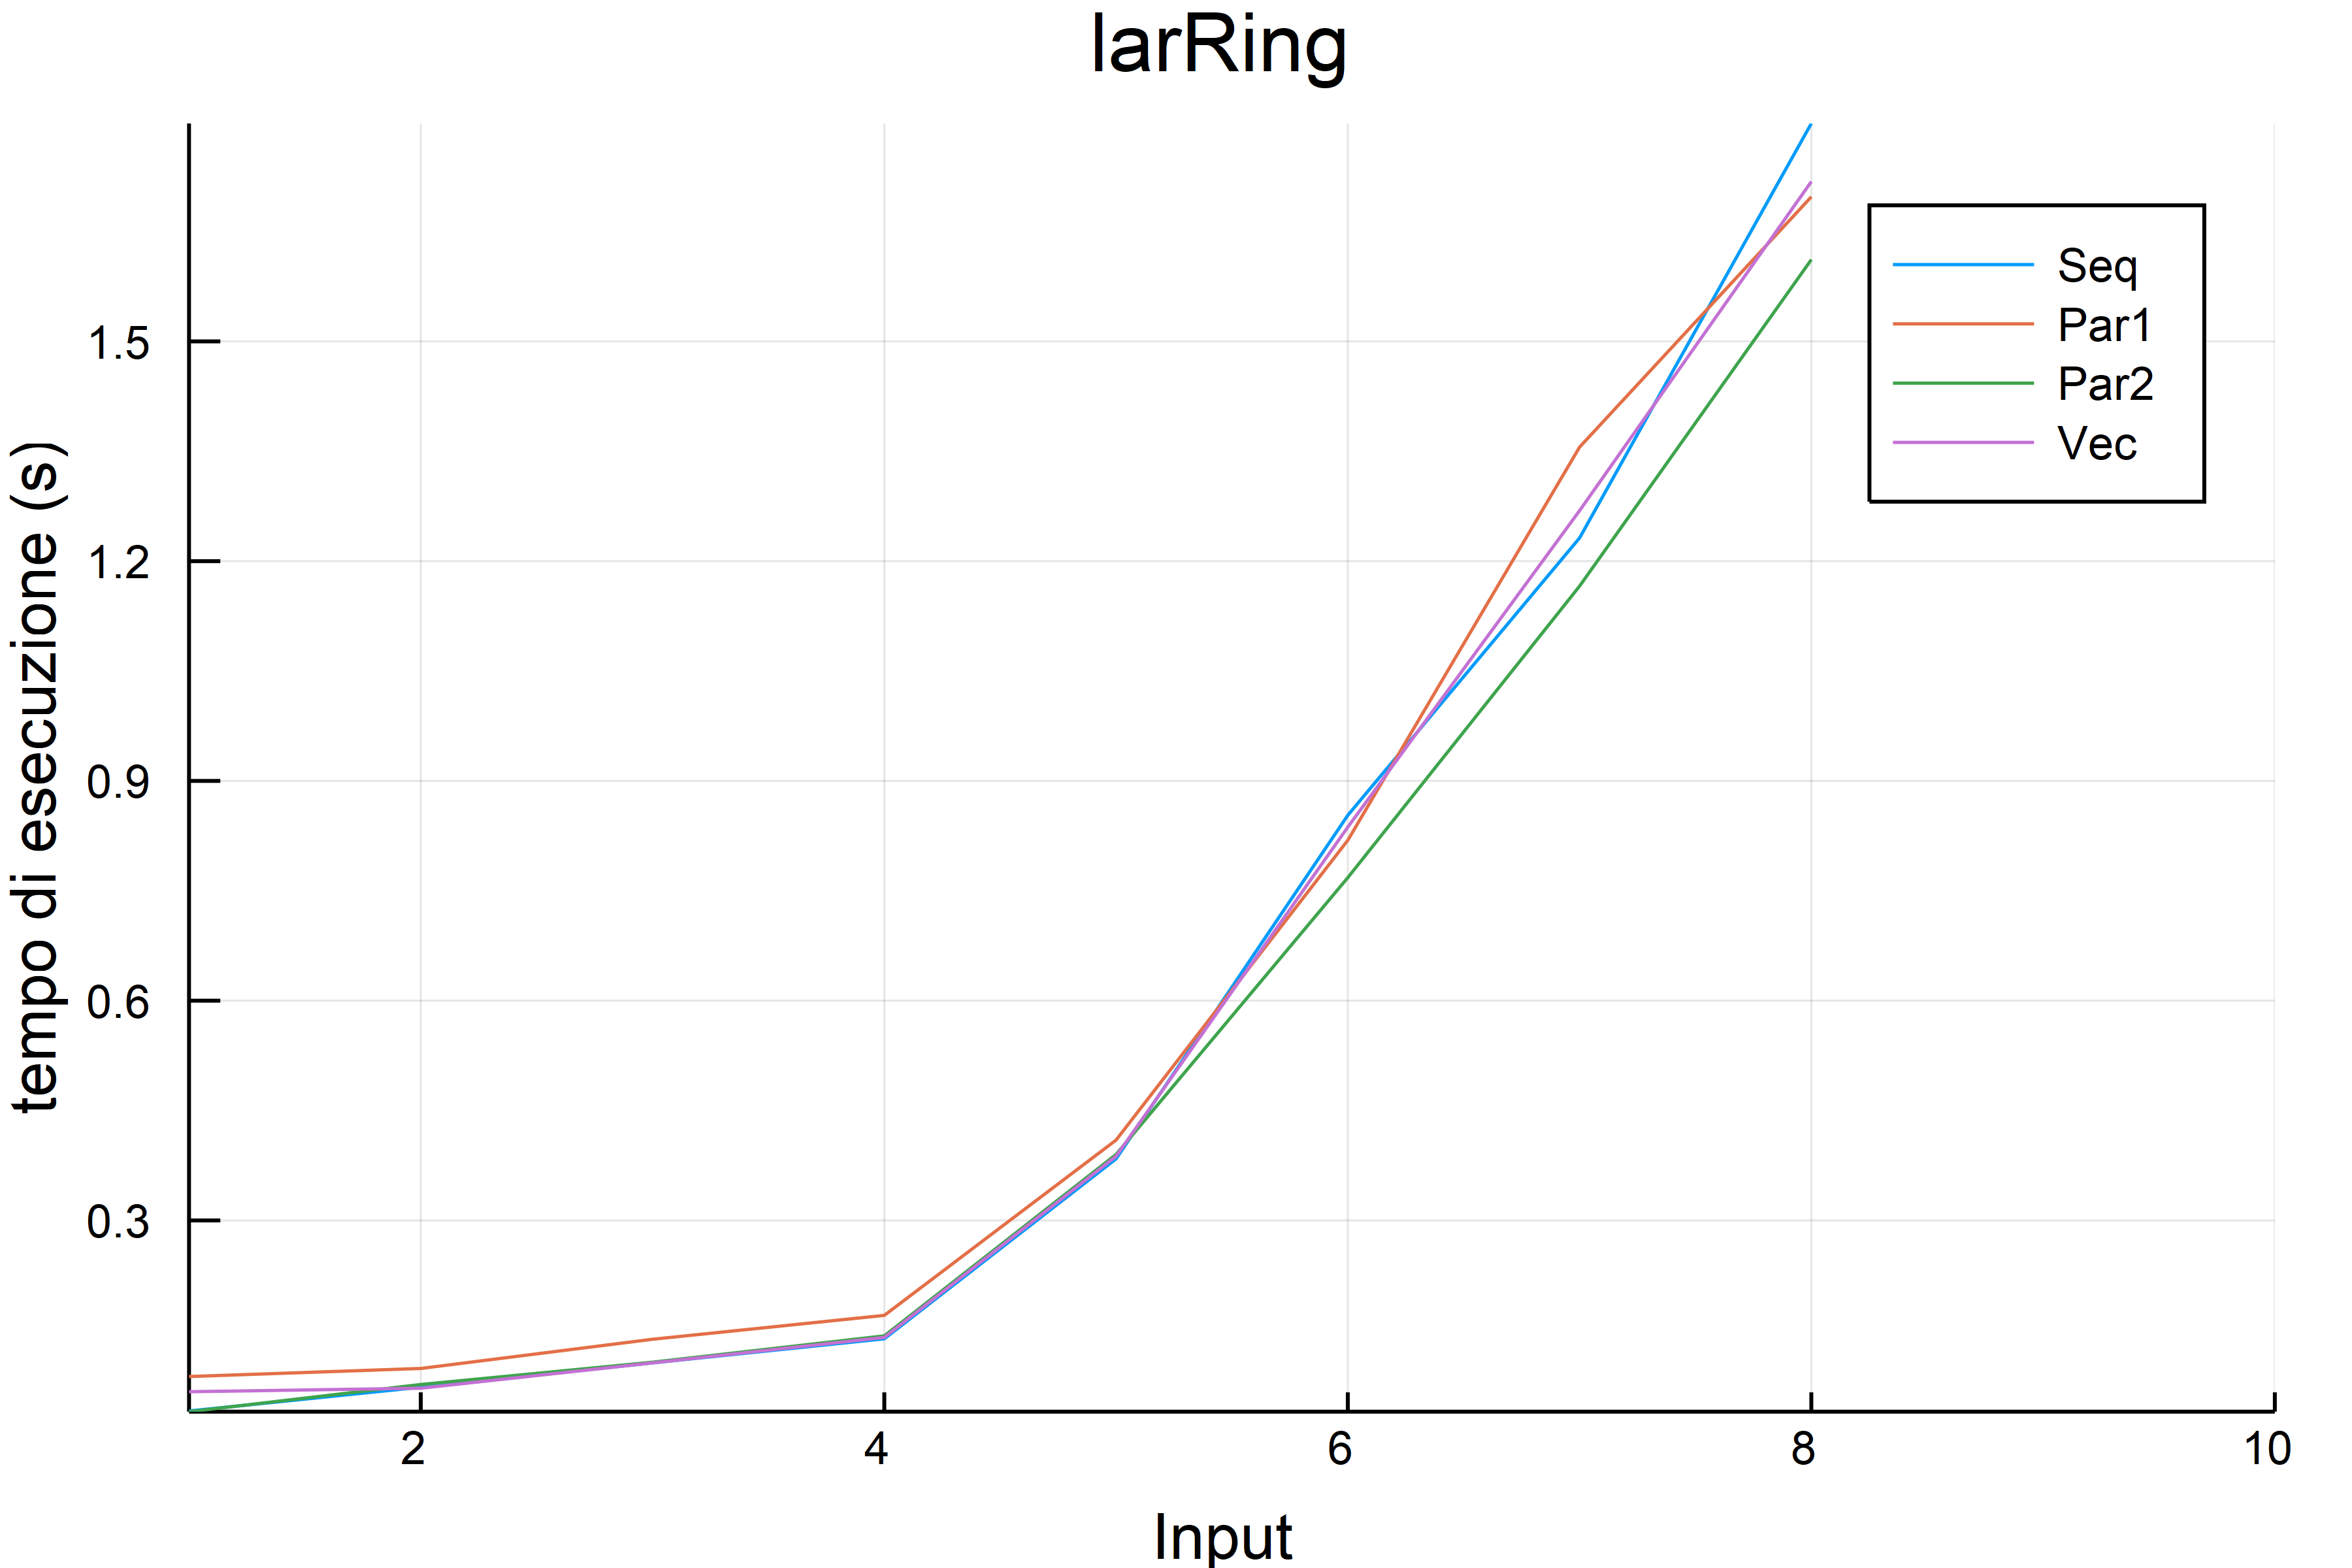
\includegraphics[scale=.13]{larRingTime.png} 
\caption{Results computed on Microsoft Surface Pro  3 (4GB LPDDR3 1600 MHz RAM, i5-4300U processor)} 
\end{figure}
%---------------------------------------------------------------------------------
\subsection{larCylinder}

\paragraph{Python}

\begin{verbatim}
def larCylinder(radius,height,angle=2*PI):
    def larCylinder0(shape=[36,1]):
        domain = larIntervals(shape)([angle,1])
        V,CV = domain
        x = lambda p : radius*COS(p[0])
        y = lambda p : radius*SIN(p[0])
        z = lambda p : height*p[1]
        mapping = [x,y,z]
        model = larMap(mapping)(domain)
    return model
return larCylinder0
\end{verbatim}

\paragraph{Julia}

\begin{verbatim}
@everywhere function larCylinder(radius,height,angle=2*pi)
    function larCylinder0(shape=[36,1])
        V,CV = LARLIB.larCuboids(shape)
        V = [angle/shape[1] 0;0 1./shape[2]]*V
        W = [V[:,k] for k=1:size(V,2)]
        Z = hcat(map(p->let(u,v)=p;[radius*cos(u);radius*sin(u);
        	height*v] end,W)...)
        return Z,CV
    end
    return larCylinder0
end
\end{verbatim}

The \textfb{larCylinder} function created a cylinder centered in the origin with given radius, height and angle.

In this case, the local parametrization used is:
$$f(u,v)=(radius*cos(u),radius*sen(u),height*v),$$
with $[u,v] \in [0,angle]\times[0,1]$.

With $$\verb!W=[V[:,k] for k=1:size(V,2)]!,$$ as opposed to $hcat$, we dispose the coordinates of the vertices (i.e. the columns in V) horizontally (into an array of arrays).

Then $map$ applies the "anonymous function" $$\verb!p->let(u,v)=p;[radius*cos(u);radius*sin(u);height*v] end!$$ to the coordinates of all the vertices contained in the W collection.

Thus a new set of vertices is created; the coordinates are disposed vertically in a matrix using the $$\verb!hcat(A...)!$$ function.

\paragraph{Visualization examples}

\begin{verbatim}
V,CV = larCylinder(1,3,2*pi)()
V
CV
V = hcat(V[:,1],[V[:,k] for k in 1:size(V,2)]...)
W = [Any[V[h,k] for h=1:size(V,1)] for k=1:size(V,2)]
hpc = p.STRUCT(p.MKPOLS(PyObject([W,CV,[]])))
p.VIEW(hpc)

V,CV = larCylinder(1,3,pi)()
V = hcat(V[:,1],[V[:,k] for k in 1:size(V,2)]...)
W = [Any[V[h,k] for h=1:size(V,1)] for k=1:size(V,2)]
hpc = p.STRUCT(p.MKPOLS(PyObject([W,CV,[]])))
p.VIEW(hpc)
\end{verbatim}

\begin{figure}[htbp] 
\centering 
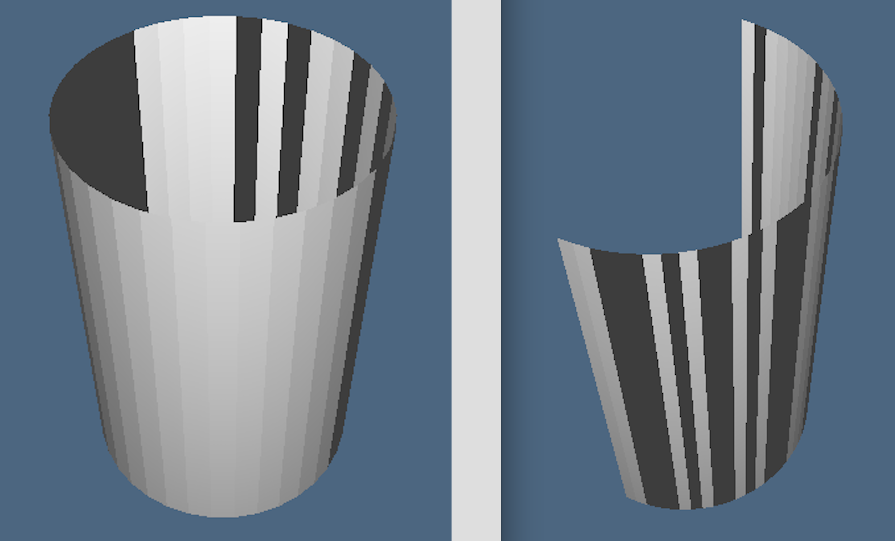
\includegraphics[scale=.29]{larCylinder.png} 
\caption{Unit radius cylinder and half cylinder on the $z$ axis of height 3.} 
\end{figure}

\paragraph{Test}

\begin{Verbatim}
@testset "larCylinder" begin
	@test BoxCalculation(larCylinder(1,5,2*pi)()[1])==20
	@test BoxCalculation(larCylinder(2,2,pi)()[1])==16
	@test BoxCalculation(larCylinder(1,4,pi)()[1])==8
	#((radius*2)^2)*height
	@test size(larCylinder(3.4,20,pi/7)()[1],2)==74
	@test length(larCylinder(3.4,20,pi/7)()[2])==36
end
\end{Verbatim}

\paragraph{Vectorization}

\begin{verbatim}
function larCylinderV(radius,height,angle=2*pi)
    function larCylinder0(shape=[36,1])
        V,CV = LARLIB.larCuboids(shape)
        V = [V[:,k] for k=1:size(V,2)]
        W = (p->[radius*cos(p[1]),radius*sin(p[1]),
            height*p[2]]).((x->[x[1]*angle/shape[1], x[2]/shape[2]]).(V))
        return hcat(W...),CV
    end
    return larCylinder0
end
\end{verbatim}

\paragraph{Parallel Computing}
\begin{Verbatim}
function larCylinderP(radius,height,angle=2*pi)
	function larCylinder0(shape=[36,1])
		V,CV = LARLIB.larCuboids(shape)
		V = SharedArray(V)
        W = SharedArray{Float64}(3,size(V,2))
        @sync @parallel for i = 1:size(V,2)
            W[1,i] = radius*cos(V[1,i]*angle/shape[1])
            W[2,i] = radius*sin(V[1,i]*angle/shape[1])
            W[3,i] = height*(V[2,i]/shape[2])
        end
        return W,CV
    end
    return larCylinder0
end 
\end{Verbatim}

\begin{Verbatim}
@everywhere function flarCylinder(W::SharedArray,V::Array,indexprt,ultim,
            shape,radius,height,angle)
    id = myid()
    if id != nprocs()
        for i=indexprt*(id-2) +1 : indexprt*(id-1)
            W[1,i] = radius*cos(V[1,i]*angle/shape[1])
            W[2,i] = radius*sin(V[1,i]*angle/shape[1])
            W[3,i] = height*(V[2,i]/shape[2]) 
        end
    else
        for i=indexprt*(id-2) +1 : ultim
            W[1,i] = radius*cos(V[1,i]*angle/shape[1])
            W[2,i] = radius*sin(V[1,i]*angle/shape[1])
            W[3,i] = height*(V[2,i]/shape[2])
        end
    end
end

function larCylinderPP(radius,height,angle=2*pi)
    function larCylinder0(shape=[36,1])
        V,CV = LARLIB.larCuboids(shape)
        W = SharedArray{Float64}(3,size(V,2))
        if nprocs() > size(V,2)
            indexprt = 1
        else
            indexprt = Int((size(V,2)-(size(V,2)%nprocs()))/nprocs())
        end
        @sync begin
            for i = 2:nprocs()
                @async remotecall_fetch(flarCylinder,i,W,V,indexprt,size(V,2),
                shape,radius,height,angle)
            end
        end
        return W,CV
    end
    return larCylinder0
end 
\end{Verbatim}

\begin{Verbatim}
@testset "Vectorized and Parallelized larCylinder" begin
    @test BoxCalculation(larCylinderV(1,5,2*pi)([56,1])[1])==20
    @test BoxCalculation(larCylinderV(2,2,pi)([56,1])[1])==16
    @test BoxCalculation(larCylinderP(2,2,pi)([56,1])[1])==16
    @test BoxCalculation(larCylinderP(1,5,2*pi)([56,1])[1])==20
    @test BoxCalculation(larCylinderPP(2,2,pi)([56,1])[1])==16
    @test BoxCalculation(larCylinderPP(1,5,2*pi)([56,1])[1])==20
end
\end{Verbatim}

\paragraph{Performance evaluation}

\begin{Verbatim}
data = [[x,1] for x in data2]

x,y = TimeGraph(larCylinder(1,2),larCylinderP(1,2),larCylinderPP(1,2),larCylinderV(1,2),data,5)
plot(x,y,yaxis=("tempo di esecuzione (s)"),xaxis=("Input",(1,length(x)+2)),
label=["Seq" "Par1" "Par2" "Vec"],title="larCylinder",lw=1) 

\end{Verbatim}

\begin{figure}[htbp] 
\centering 
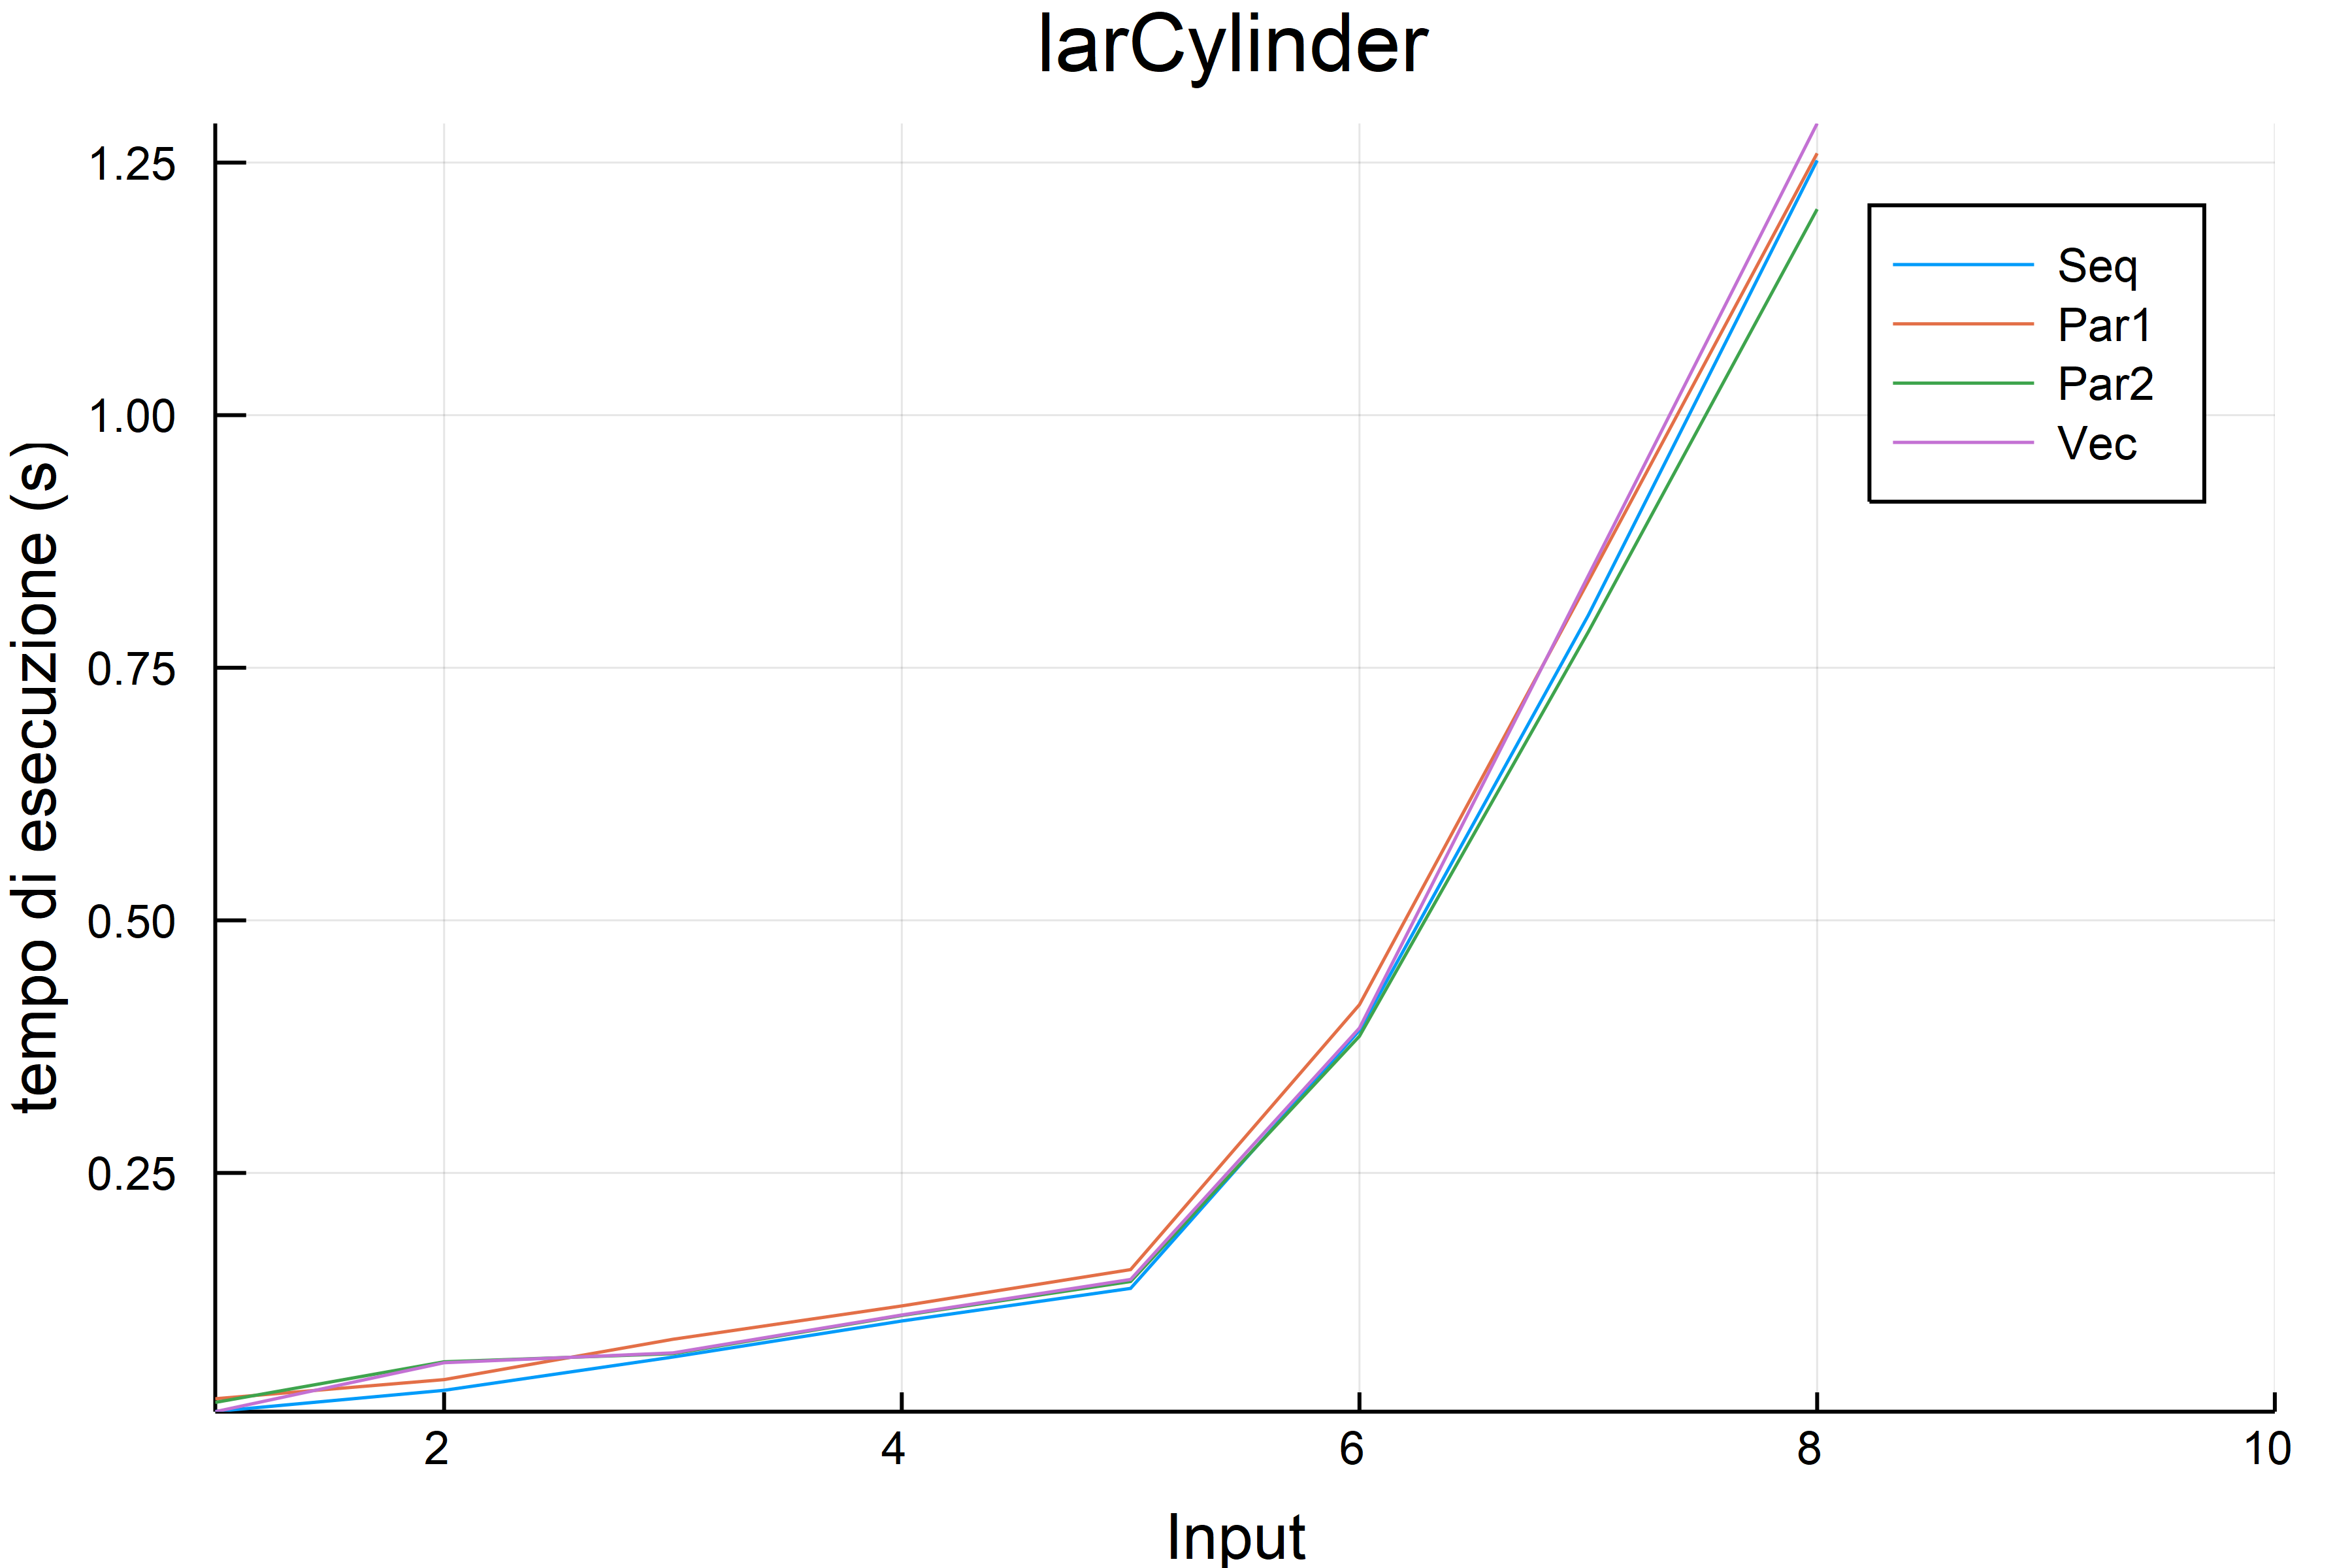
\includegraphics[scale=.13]{larCylinderTime.png} 
\caption{Results computed on Microsoft Surface Pro  3 (4GB LPDDR3 1600 MHz RAM, i5-4300U processor)} 
\end{figure}

%---------------------------------------------------------------------------------
\subsection{larSphere}

\paragraph{Python}

\begin{verbatim}
def larSphere(radius=1,angle1=PI,angle2=2*PI):
    def larSphere0(shape=[18,36]):
        V,CV = larIntervals(shape,'simplex')([angle1,angle2])
        V = larTranslate([-angle1/2,-angle2/2])(V)
        domain = V,CV
        x = lambda p : radius*COS(p[0])*COS(p[1])
        y = lambda p : radius*COS(p[0])*SIN(p[1])
        z = lambda p : radius*SIN(p[0])
        return larMap([x,y,z])(domain)
    return larSphere0
\end{verbatim}

\paragraph{Julia}

\begin{verbatim}
@everywhere function larSphere(radius=1,angle1=pi,angle2=2*pi)
    function larSphere0(shape=[18,36])
        V,CV = larSimplexGrid1(shape)
        V = [angle1/shape[1] 0;0 angle2/shape[2]]*V
        V = broadcast(+,V,[-angle1/2,-angle2/2])
        W = [V[:,k] for k=1:size(V,2)]
        X = hcat(map(p->let(u,v)=p;[radius*cos(u)*cos(v);
        	radius*cos(u)*sin(v);radius*sin(u)]end,W)...) 
    return X,CV
    end
    return larSphere0    
end
\end{verbatim}

The \textfb{larSphere} function creates a sphere centered in the origin with given radius and angles. 

In this case, the local parametrization used is:
$$f(u,v)=(radius*cos(u)*cos(v);radius*cos(u)*sin(v);radius*sin(u)),$$
with $[u,v] \in [-\frac{angle1}{2},\frac{angle1}{2}]\times[-\frac{angle2}{2},\frac{angle2}{2}]$.

With $$\verb!V=broadcast(+,V,[-angle1/2,-angle2/2])!$$ we sum $-\frac{angle_1}{2}$ to every element in the first row of V and $-\frac{angle_2}{2}$ to every element in the second row of V.

With $$\verb!W=[V[:,k] for k=1:size(V,2)]!,$$ as opposed to $hcat$, we dispose the coordinates of the vertices (i.e. the columns in V) horizontally (into an array of arrays).

Then $map$ applies the "anonymous function" $$\verb!p->let(u,v)=p;[radius*cos(u)*cos(v);radius*cos(u)*sin(v);radius*sin(u)]end!$$ to the coordinates of all the vertices contained in the W collection. Next, with the $hcat$ function, the coordinates of the new vertices are rearranged vertically in a matrix.

\paragraph{Visualization examples}

\begin{verbatim}
V,CV = larSphere(1,pi,2*pi)()
V
CV
W = [Any[V[h,k] for h=1:size(V,1)] for k=1:size(V,2)]
hpc = p.STRUCT(p.MKPOLS(PyObject([W,CV,[]])))
p.VIEW(hpc)

V,CV = larSphere(1,pi,pi)()
W = [Any[V[h,k] for h=1:size(V,1)] for k=1:size(V,2)]
hpc = p.STRUCT(p.MKPOLS(PyObject([W,CV,[]])))
p.VIEW(hpc)
\end{verbatim}

\begin{figure}[htbp] 
\centering 
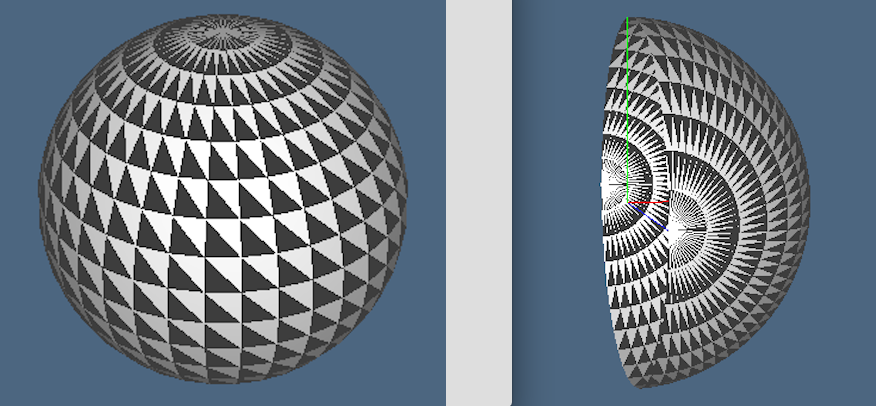
\includegraphics[scale=.32]{larSphere.png} 
\caption{Unit radius spherical surface and half spherical surface centered in the origin.} 
\end{figure}

\paragraph{Test}
\begin{Verbatim}
@testset "larSphere" begin
	@test BoxCalculation(larSphere(2,pi,2*pi)()[1])==64
	@test BoxCalculation(larSphere(6,pi,pi)()[1])==864
	@test BoxCalculation(larSphere(4,pi,2*pi)()[1])==8^3
	#(radius*2)^3
	@test size(larSphere(2.5,pi/3,pi/5)()[1],2)==703
	@test length(larSphere(2.5,pi/3,pi/5)()[2])==1296
end
\end{Verbatim}

\paragraph{Vectorization}

\begin{verbatim}
function larSphereV(radius=1,angle1=pi,angle2=2*pi)
    function larSphere0(shape=[18,36])
        V,CV = larSimplexGrid1(shape)
        V = [V[:,k] for k=1:size(V,2)]
        W = (p->[radius*cos(p[1])*cos(p[2]),radius*cos(p[1])*sin(p[2]),
            radius*sin(p[1])]).((x->x+[-angle1/2,-angle2/2]).((x->[x[1]*angle1/shape[1],
            x[2]*angle2/shape[2]]).(V)))
    return hcat(W...),CV
    end
    return larSphere0    
end
\end{verbatim}

\paragraph{Parallel Computing}
\begin{Verbatim}
function larSphereP(radius=1,angle1=pi,angle2=2*pi)
    function larSphere0(shape=[18,36])
        V,CV = larSimplexGrid1(shape)
        V = SharedArray(V)
        W = SharedArray{Float64}(3,size(V,2))
        @sync @parallel for i = 1:size(V,2)
            W[1,i] = radius*cos(V[1,i]*angle1/shape[1]-(angle1/2))*
            cos(V[2,i]*angle2/shape[2]-(angle2/2))
            W[2,i] = radius*cos(V[1,i]*angle1/shape[1]-(angle1/2))*
            sin(V[2,i]*angle2/shape[2]-(angle2/2))
            W[3,i] = radius*sin(V[1,i]*
            angle1/shape[1]-(angle1/2))
        end
        return W,CV
    end
    return larSphere0    
end
\end{Verbatim}

\begin{Verbatim}
@everywhere function flarSphere(W::SharedArray,V::Array,indexprt,ultim,shape,
            radius,angle1,angle2)
    id = myid()
    if id != nprocs()
        for i=indexprt*(id-2) +1 : indexprt*(id-1)
            W[1,i] = radius*cos(V[1,i]*angle1/shape[1]-(angle1/2))*
            cos(V[2,i]*angle2/shape[2]-(angle2/2))
            W[2,i] = radius*cos(V[1,i]*angle1/shape[1]-(angle1/2))*
            sin(V[2,i]*angle2/shape[2]-(angle2/2))
            W[3,i] = radius*sin(V[1,i]*angle1/shape[1]-(angle1/2))
        end
    else
        for i=indexprt*(id-2) +1 : ultim
            W[1,i] = radius*cos(V[1,i]*angle1/shape[1]-(angle1/2))*
            cos(V[2,i]*angle2/shape[2]-(angle2/2))
            W[2,i] = radius*cos(V[1,i]*angle1/shape[1]-(angle1/2))*
            sin(V[2,i]*angle2/shape[2]-(angle2/2))
            W[3,i] = radius*sin(V[1,i]*angle1/shape[1]-(angle1/2))
        end
    end
end

function larSpherePP(radius=1,angle1=pi,angle2=2*pi)
    function larSphere0(shape=[18,36])
        V,CV = larSimplexGrid1(shape)
        W = SharedArray{Float64}(3,size(V,2))
        if nprocs() > size(V,2)
            indexprt = 1
        else
            indexprt = Int((size(V,2)-(size(V,2)%nprocs()))/nprocs())
        end
        @sync begin
            for i = 2:nprocs()
                @async remotecall_fetch(flarSphere,i,W,V,indexprt,size(V,2),
                shape,radius,angle1,angle2)
            end
        end
        return W,CV
    end
    return larSphere0    
end
\end{Verbatim}

\begin{Verbatim}
@testset "Vectorized and Parallelized larSphere" begin
    @test BoxCalculation(larSphereV(2,pi,2*pi)()[1])==64
    @test BoxCalculation(larSphereV(6,pi,pi)()[1])==864
    @test BoxCalculation(larSphereP(2,pi,2*pi)()[1])==64
    @test BoxCalculation(larSphereP(6,pi,pi)()[1])==864
    @test BoxCalculation(larSpherePP(2,pi,2*pi)()[1])==64
    @test BoxCalculation(larSpherePP(6,pi,pi)()[1])==864
end
\end{Verbatim}

\paragraph{Performance evaluation}

\begin{Verbatim}
data = [[x,1] for x in data3]

x,y = TimeGraph(larSphere(),larSphereP(),larSpherePP(),larSphereV(),data,5)
plot(x,y,yaxis=("tempo di esecuzione (s)"),xaxis=("Input",(1,length(x)+2)),
label=["Seq" "Par1" "Par2" "Vec"],title="larSphere",lw=1)

\end{Verbatim}

\begin{figure}[htbp] 
\centering 
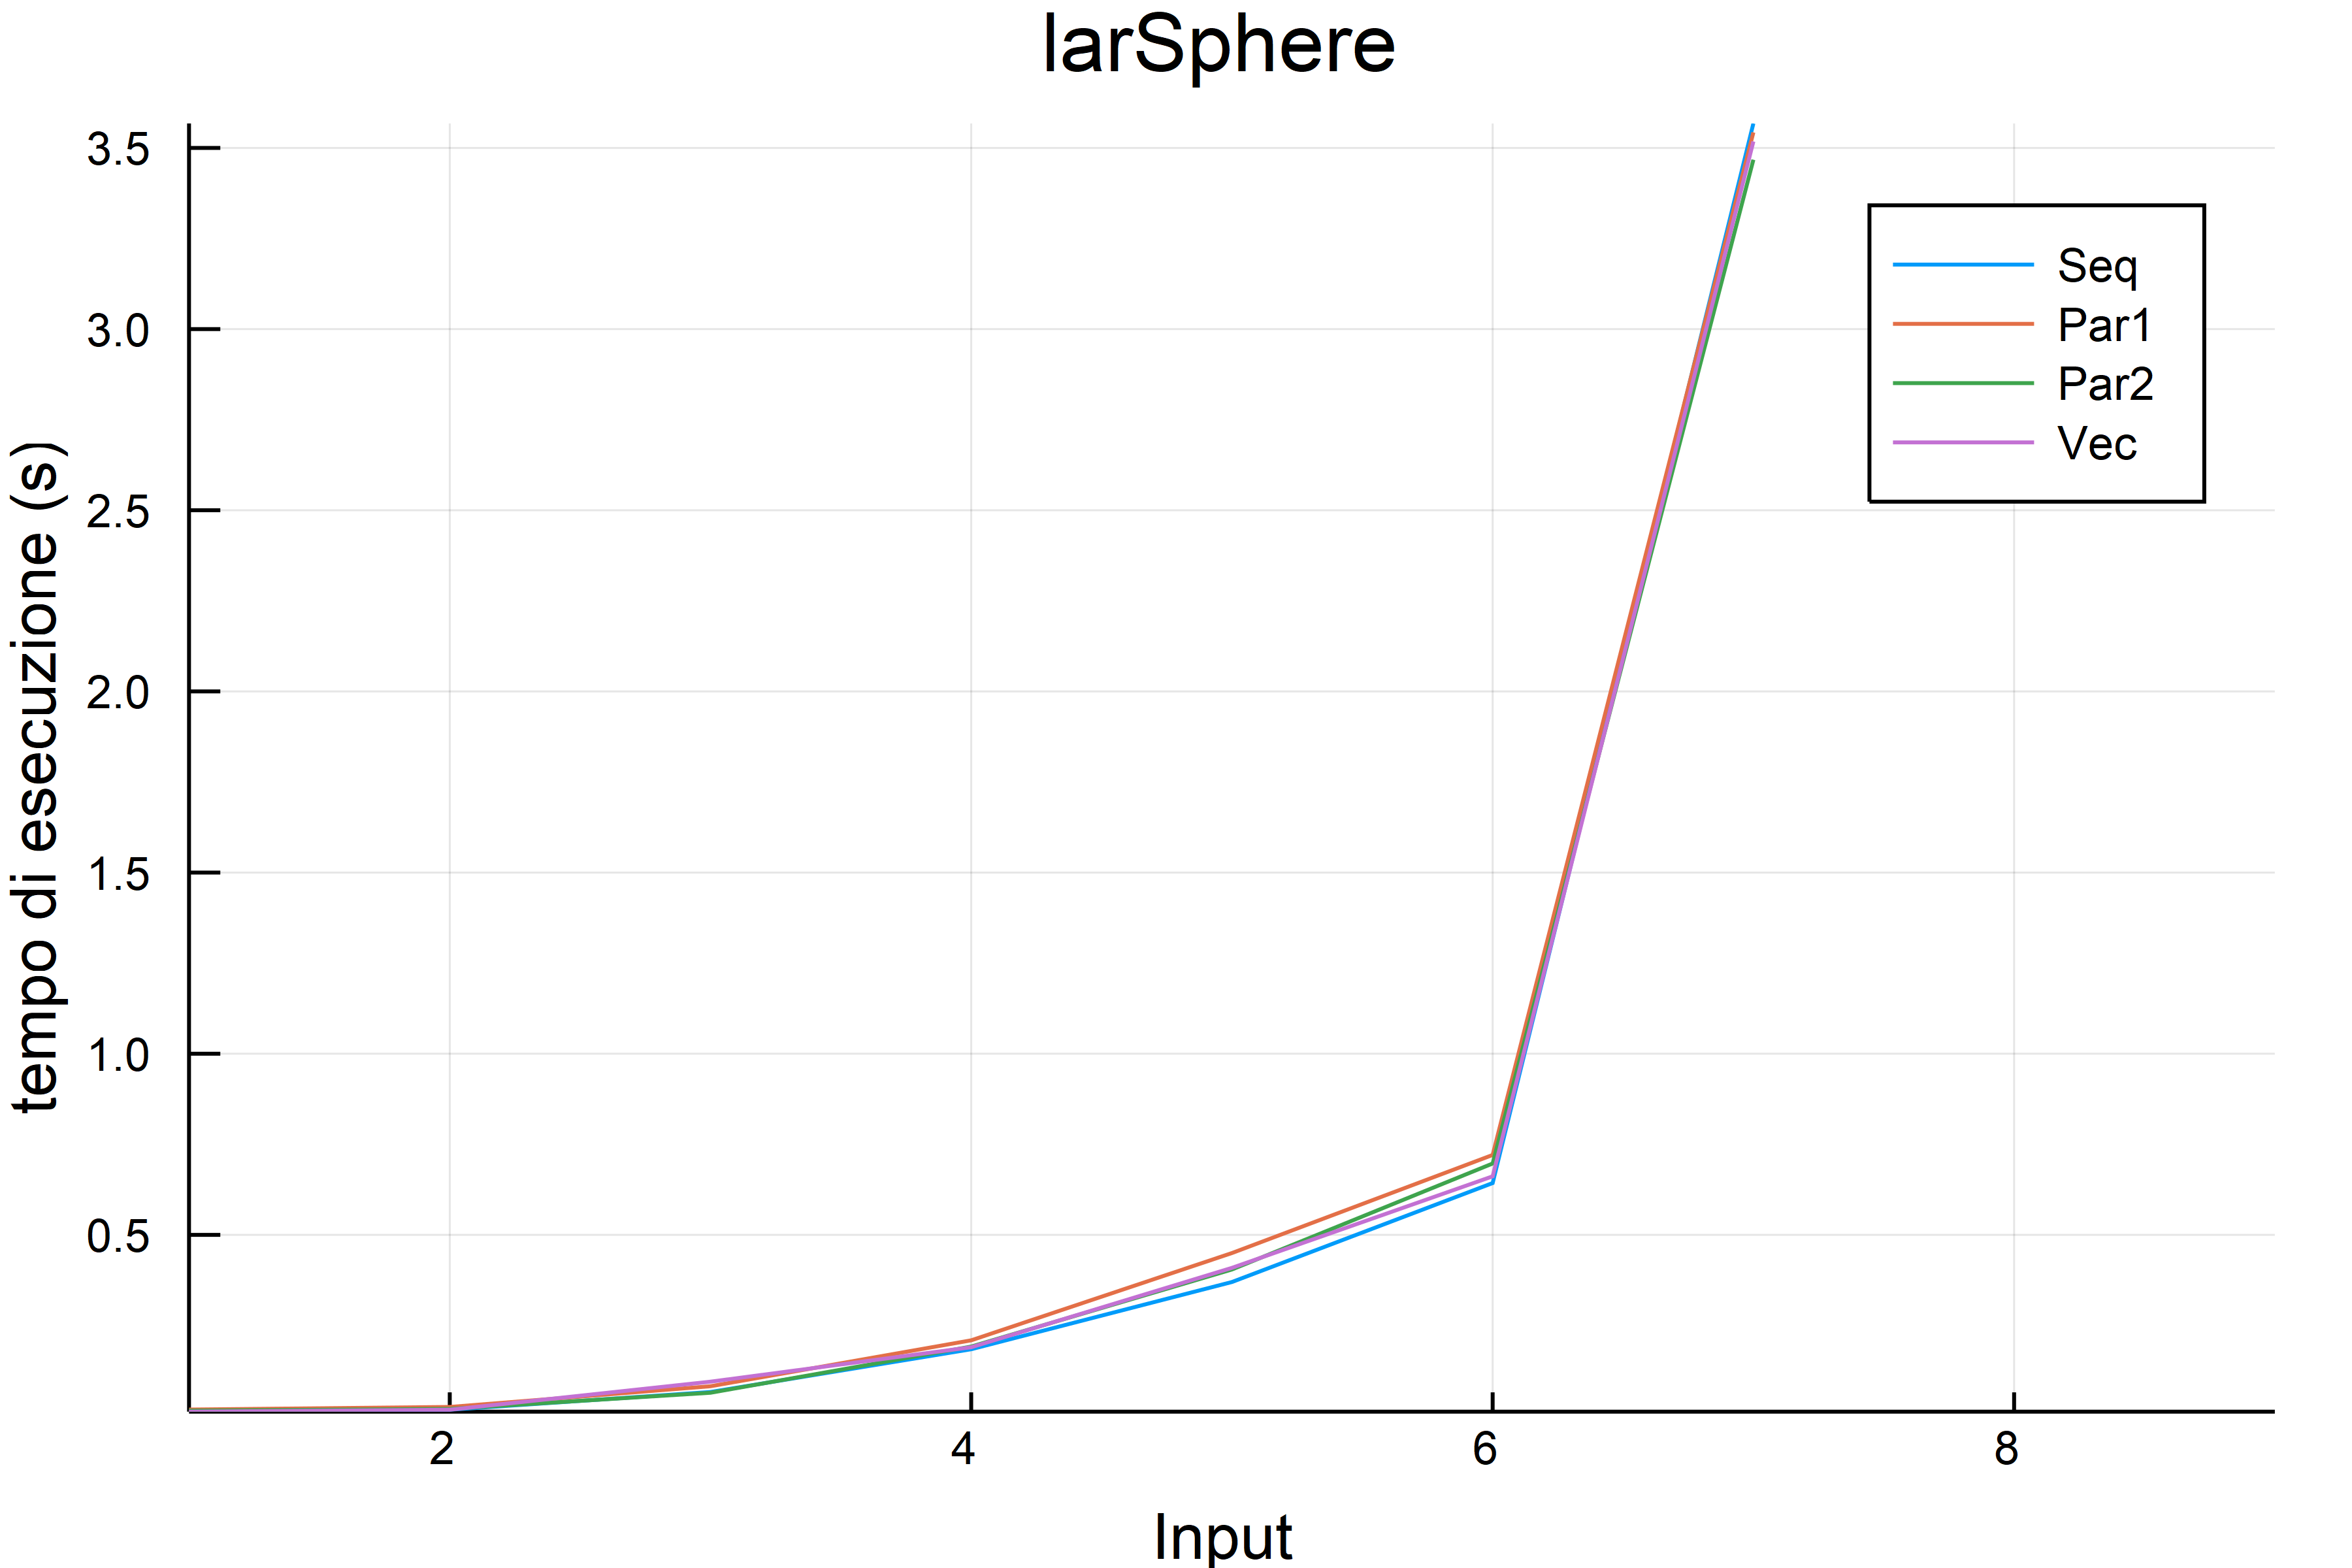
\includegraphics[scale=.13]{larSphereTime.png} 
\caption{Results computed on Microsoft Surface Pro  3 (4GB LPDDR3 1600 MHz RAM, i5-4300U processor)} 
\end{figure}

%---------------------------------------------------------------------------------
\subsection{larToroidal}

\paragraph{Python}

\begin{verbatim}
def larToroidal(r,R,angle1=2*PI,angle2=2*PI):
    def larToroidal0(shape=[24,36]):
        domain = larIntervals(shape,'simplex')([angle1,angle2])
        V,CV = domain
        x = lambda p : (R + r*COS(p[0])) * COS(p[1])
        y = lambda p : (R + r*COS(p[0])) * SIN(p[1])
        z = lambda p : -r * SIN(p[0])
        return larMap([x,y,z])(domain)
    return larToroidal0
\end{verbatim}

\paragraph{Julia}

\begin{verbatim}
function larToroidal(r=1,R=2,angle1=2*pi,angle2=2*pi)
    function larToroidal0(shape=[24,36])
        V,CV = larSimplexGrid1(shape)
        V = [angle1/shape[1] 0;0 angle2/shape[2]]*V
        W = [V[:,k] for k=1:size(V,2)]
        X = hcat(map(p->let(u,v)=p;[(R+r*cos(u))*cos(v);
        	(R+r*cos(u))*sin(v);-r*sin(u)]end,W)...) 
        return X,CV
    end
    return larToroidal0    
end
\end{verbatim}

The \textfb{larToroidal} function creates a torus with given radiuses (radius of the circle that generates the torus and distance from the origin) and angles.

In this case, the local parametrization used is:
$$f(u,v)=(R+rcos(u)cos(v),R+rcos(u)sen(v),-rsen(u)),$$
with $[u,v] \in [0,angle1]\times[0,angle2]$.

With $$\verb!W=[V[:,k] for k=1:size(V,2)]!,$$ as opposed to $hcat$, we dispose the coordinates of the vertices (i.e. the columns in V) horizontally (into an array of arrays).

Then $map$ applies the "anonymous function" $$\verb!p->let(u,v)=p;[(R+r*cos(u))*cos(v);(R+r*cos(u))*sin(v);-r*sin(u)]end!$$ to the coordinates of all the vertices contained in the W collection. Next, with the $hcat$ function, the coordinates of the new vertices are rearranged vertically in a matrix.

\paragraph{Visualization examples}

\begin{verbatim}
V,CV = larToroidal(1,2,2*pi,2*pi)()
V
CV
W = [Any[V[h,k] for h=1:size(V,1)] for k=1:size(V,2)]
hpc = p.STRUCT(p.MKPOLS(PyObject([W,CV,[]])))
p.VIEW(hpc)

V,CV = larToroidal(1,2,pi,2*pi)()
W = [Any[V[h,k] for h=1:size(V,1)] for k=1:size(V,2)]
hpc = p.STRUCT(p.MKPOLS(PyObject([W,CV,[]])))
p.VIEW(hpc)
\end{verbatim}

\begin{figure}[htbp] 
\centering 
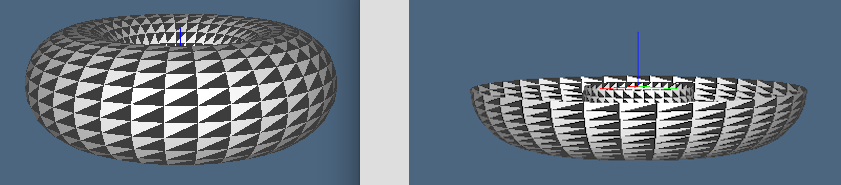
\includegraphics[scale=.43]{larToroidal.png} 
\caption{Torus centered in the origin of radiuses 1 and 2 with its horizontal section.} 
\end{figure}

\paragraph{Test}
\begin{Verbatim}
@testset "larToroidal" begin
	@test BoxCalculation(larToroidal(1,3,2*pi,2*pi)()[1])==128
	@test BoxCalculation(larToroidal(2,3,2*pi,2*pi)()[1])==400
	#(((R+r)*2)^2)*(r*2)
	@test size(larToroidal(1.3,4.6,pi/4,pi/7)()[1],2)==925
	@test length(larToroidal(1.3,4.6,pi/4,pi/7)()[2])==1728
end
\end{Verbatim}

\paragraph{Vectorization}

\begin{verbatim}
function larToroidalV(r=1,R=2,angle1=2*pi,angle2=2*pi)
    function larToroidal0(shape=[24,36])
        V,CV = larSimplexGrid1(shape)
        V = [V[:,k] for k=1:size(V,2)]
        W = (p->[(R+r*cos(p[1]))*cos(p[2]),(R+r*cos(p[1]))*sin(p[2]),
            -r*sin(p[1])]).((x->[x[1]*angle1/shape[1], x[2]*angle2/shape[2]]).(V))
        return hcat(W...),CV
    end
    return larToroidal0    
end
\end{verbatim}

\paragraph{Parallel Computing}
\begin{Verbatim}
function larToroidalP(r=1,R=2,angle1=2*pi,angle2=2*pi)
    function larToroidal0(shape=[24,36])
        V,CV = larSimplexGrid1(shape)
        V = SharedArray(V)
        W = SharedArray{Float64}(3,size(V,2))           
        @sync @parallel for i = 1:size(V,2)
            W[1,i] = (R+r*cos(V[1,i]*angle1/shape[1]))*cos(V[2,i]*angle2/shape[2])           
            W[2,i] = (R+r*cos(V[1,i]*angle1/shape[1]))*sin(V[2,i]*angle2/shape[2])
            W[3,i] = -r*sin(V[1,i]*angle1/shape[1])
        end
        return W,CV
    end
    return larToroidal0    
end 
\end{Verbatim}

\begin{Verbatim}
@everywhere function flarToroidal(W::SharedArray,V::Array,indexprt,ultim,
            shape,r,R,angle1,angle2)
    id = myid()
    if id != nprocs()
        for i=indexprt*(id-2) +1 : indexprt*(id-1)
            W[1,i] = (R+r*cos(V[1,i]*angle1/shape[1]))*cos(V[2,i]*angle2/shape[2])           
            W[2,i] = (R+r*cos(V[1,i]*angle1/shape[1]))*sin(V[2,i]*angle2/shape[2])
            W[3,i] = -r*sin(V[1,i]*angle1/shape[1])
        end
    else
        for i=indexprt*(id-2) +1 : ultim
            W[1,i] = (R+r*cos(V[1,i]*angle1/shape[1]))*cos(V[2,i]*angle2/shape[2])           
            W[2,i] = (R+r*cos(V[1,i]*angle1/shape[1]))*sin(V[2,i]*angle2/shape[2])
            W[3,i] = -r*sin(V[1,i]*angle1/shape[1])
        end
    end
end

function larToroidalPP(r=1,R=2,angle1=2*pi,angle2=2*pi)
    function larToroidal0(shape=[24,36])
        V,CV = larSimplexGrid1(shape)
        W = SharedArray{Float64}(3,size(V,2))           
        if nprocs() > size(V,2)
            indexprt = 1
        else
            indexprt = Int((size(V,2)-(size(V,2)%nprocs()))/nprocs())
        end
        @sync begin
            for i = 2:nprocs()
                @async remotecall_fetch(flarToroidal,i,W,V,indexprt,size(V,2),
                shape,r,R,angle1,angle2)
            end
        end
        return W,CV
    end
    return larToroidal0    
end 
\end{Verbatim}

\begin{Verbatim}
@testset "Vectorized and Parallelized larToroidal" begin
    @test BoxCalculation(larToroidalV(1,3,2*pi,2*pi)()[1])==128
    @test BoxCalculation(larToroidalV(2,3,2*pi,2*pi)()[1])==400
    @test BoxCalculation(larToroidalPP(2,3,2*pi,2*pi)()[1])==400
    @test BoxCalculation(larToroidalPP(1,3,2*pi,2*pi)()[1])==128
    @test BoxCalculation(larToroidalP(2,3,2*pi,2*pi)()[1])==400
    @test BoxCalculation(larToroidalP(1,3,2*pi,2*pi)()[1])==128
end
\end{Verbatim}

\paragraph{Performance evaluation}

\begin{Verbatim}
data = [[x,1] for x in data3]

x,y = TimeGraph(larToroidal(),larToroidalP(),larToroidalPP(),larToroidalV(),data,5)
plot(x,y,yaxis=("tempo di esecuzione (s)"),xaxis=("Input",(1,length(x)+2)),
label=["Seq" "Par1" "Par2" "Vec"],title="larToroidal",lw=1)

\end{Verbatim}

\begin{figure}[htbp] 
\centering 
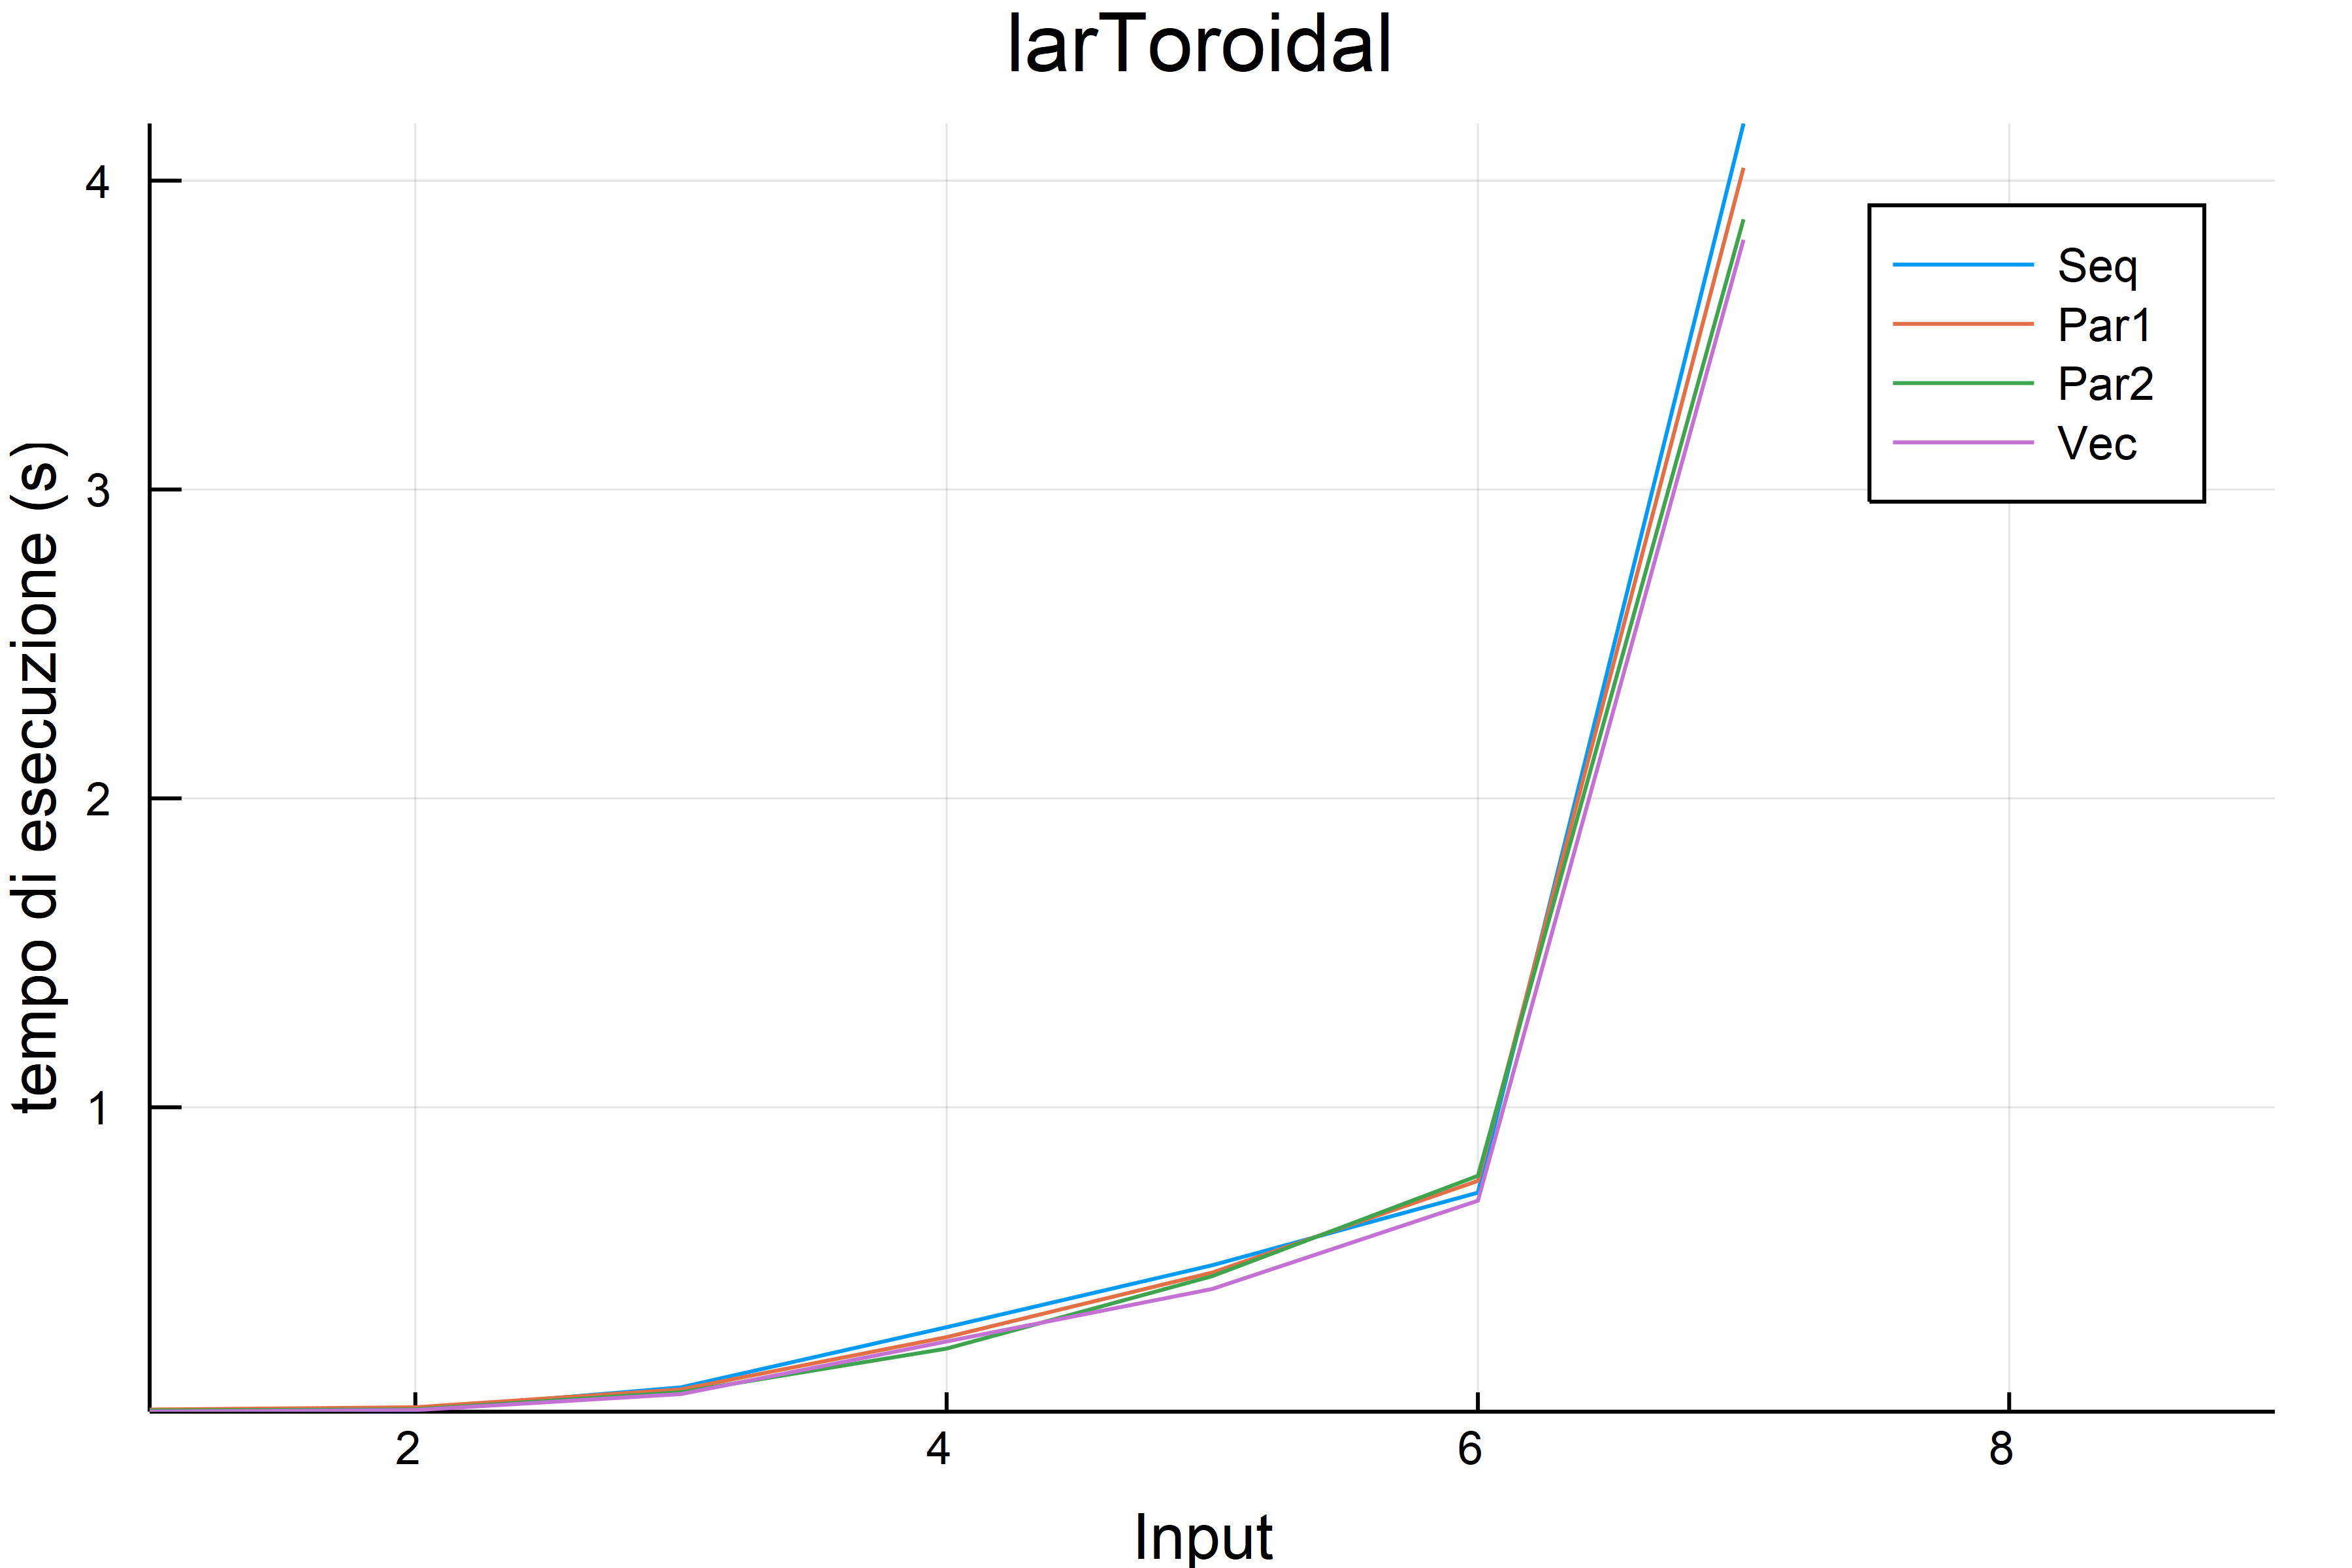
\includegraphics[scale=.13]{larToroidalTime.png} 
\caption{Results computed on Microsoft Surface Pro  3 (4GB LPDDR3 1600 MHz RAM, i5-4300U processor)} 
\end{figure}

%---------------------------------------------------------------------------------
\subsection{larCrown}

\paragraph{Python}

\begin{verbatim}
def larCrown(r,R,angle=2*PI):
    def larCrown0(shape=[24,36]):
        V,CV = larIntervals(shape,'simplex')([PI,angle])
        V = larTranslate([-PI/2,0])(V)
        domain = V,CV
        x = lambda p : (R + r*COS(p[0])) * COS(p[1])
        y = lambda p : (R + r*COS(p[0])) * SIN(p[1])
        z = lambda p : -r * SIN(p[0])
        return larMap([x,y,z])(domain)
    return larCrown0
\end{verbatim}

\paragraph{Julia}

\begin{verbatim}
@everywhere function larCrown(r=1,R=2,angle=2*pi)
    function larCrown0(shape=[24,36])
        V,CV = larSimplexGrid1(shape)
        V = [pi/shape[1] 0;0 angle/shape[2]]*V
        V = broadcast(+,V,[-pi/2,0])
        W = [V[:,k] for k=1:size(V,2)]
        X = hcat(map(p->let(u,v)=p;[(R+r*cos(u))*cos(v);
       	(R+r*cos(u))*sin(v);-r*sin(u)]end,W)...)
       return X,CV
    end
    return larCrown0    
end
\end{verbatim}

The \textfb{larCrown} function creates an outer shell of torus with given radiuses and angle.

In this case, the local parametrization used is:
$$f(u,v)=(R+rcos(u)cos(v),R+rcos(u)sen(v),-rsen(u)),$$
with $[u,v] \in [-\frac{\pi}{2},\frac{\pi}{2}]\times[0,angle]$.

With $$\verb!V=broadcast(+,V,[-pi/2,0])!$$ we sum $-\frac{\pi}{2}$ to each element in the first row of V and 0 to every element in the second row of V.

With $$\verb!W=[V[:,k] for k=1:size(V,2)]!,$$ as opposed to $hcat$, we dispose the coordinates of the vertices (i.e. the columns in V) horizontally (into an array of arrays).

Then $map$ applies the "anonymous function" $$\verb!p->let(u,v)=p[radius*cos(u)*cos(v);radius*cos(u)*sin(v);radius*sin(u)]end!$$ to the coordinates of all the vertices contained in the W collection. Next, with the $hcat$ function, the coordinates of the new vertices are rearranged vertically in a matrix.

\paragraph{Visualization examples}

\begin{verbatim}
V,CV = larCrown(1,3,2*pi)()
V
CV
W = [Any[V[h,k] for h=1:size(V,1)] for k=1:size(V,2)]
hpc = p.STRUCT(p.MKPOLS(PyObject([W,CV,[]])))
p.VIEW(hpc)

V,CV = larCrown(1,3,pi)()
W = [Any[V[h,k] for h=1:size(V,1)] for k=1:size(V,2)]
hpc = p.STRUCT(p.MKPOLS(PyObject([W,CV,[]])))
p.VIEW(hpc)
\end{verbatim}

\begin{figure}[htbp] 
\centering 
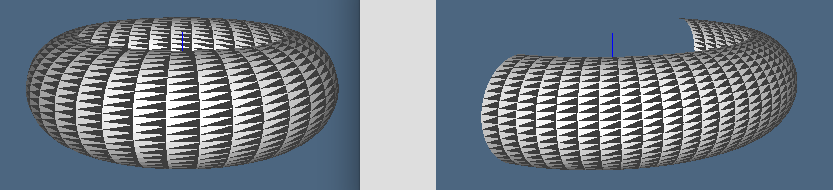
\includegraphics[scale=.46]{larCrown.png} 
\caption{Torus outer shell centered in the origin of radiuses 1 and 3, with its vertical section.} 
\end{figure}

\paragraph{Test}
\begin{Verbatim}
@testset "larCrown" begin
	@test BoxCalculation(larCrown(1,3,2*pi)()[1])==128
	@test BoxCalculation(larCrown(2,3,2*pi)()[1])==400
	#(((R+r)*2)^2)*(r*2)
	@test size(larCrown(1.5,5.6,pi/8)()[1],2)==925
	@test length(larCrown(1.5,5.6,pi/8)()[2])==1728
end
\end{Verbatim}

\paragraph{Vectorization}

\begin{verbatim}
function larCrownV(r=1,R=2,angle=2*pi)
    function larCrown0(shape=[24,36])
        V,CV = larSimplexGrid1(shape)
        V = [V[:,k] for k=1:size(V,2)]
        W = (p->[(R+r*cos(p[1]))*cos(p[2]);(R+r*cos(p[1]))*sin(p[2]);
            -r*sin(p[1])]).((x->[x[1]*pi/shape[1]-pi/2, x[2]*angle/shape[2]]).(V))
        return hcat(W...),CV
    end
    return larCrown0    
end
\end{verbatim}

\paragraph{Parallel Computing}
\begin{Verbatim}
function larCrownP(r=1,R=2,angle=2*pi)          
    function larCrown0(shape=[24,36])
        V,CV = larSimplexGrid1(shape)
        V = SharedArray(V)
        W = SharedArray{Float64}(3,size(V,2))           
        @sync @parallel for i = 1:size(V,2)
            W[1,i] = (R+r*cos(V[1,i]*pi/shape[1]-pi/2))*cos(V[2,i]*angle/shape[2])           
            W[2,i] = (R+r*cos(V[1,i]*pi/shape[1]-pi/2))*sin(V[2,i]*angle/shape[2])
            W[3,i] = -r*sin(V[1,i]*pi/shape[1]-pi/2)
        end
        return W,CV
    end
    return larCrown0    
end
\end{Verbatim}

\begin{Verbatim}
@everywhere function flarCrown(W::SharedArray,V::Array,indexprt,ultim,shape,r,R,angle)
    id = myid()
    if id != nprocs()
        for i=indexprt*(id-2) +1 : indexprt*(id-1)
            W[1,i] = (R+r*cos(V[1,i]*pi/shape[1]-pi/2))*cos(V[2,i]*angle/shape[2])           
            W[2,i] = (R+r*cos(V[1,i]*pi/shape[1]-pi/2))*sin(V[2,i]*angle/shape[2])
            W[3,i] = -r*sin(V[1,i]*pi/shape[1]-pi/2)
        end
    else
        for i=indexprt*(id-2) +1 : ultim
            W[1,i] = (R+r*cos(V[1,i]*pi/shape[1]-pi/2))*cos(V[2,i]*angle/shape[2])           
            W[2,i] = (R+r*cos(V[1,i]*pi/shape[1]-pi/2))*sin(V[2,i]*angle/shape[2])
            W[3,i] = -r*sin(V[1,i]*pi/shape[1]-pi/2)
        end
    end
end

function larCrownPP(r=1,R=2,angle=2*pi)          
    function larCrown0(shape=[24,36])
        V,CV = larSimplexGrid1(shape)
        W = SharedArray{Float64}(3,size(V,2))           
        if nprocs() > size(V,2)
            indexprt = 1
        else
            indexprt = Int((size(V,2)-(size(V,2)%nprocs()))/nprocs())
        end
        @sync begin
            for i = 2:nprocs()
                @async remotecall_fetch(flarCrown,i,W,V,indexprt,size(V,2),
                shape,r,R,angle)
            end
        end
        return W,CV
    end
    return larCrown0    
end
\end{Verbatim}

\begin{Verbatim}
@testset "Vectorized and Parallelized larCrown" begin
    @test BoxCalculation(larCrownV(1,3,2*pi)()[1])==128
    @test BoxCalculation(larCrownV(2,3,2*pi)()[1])==400
    @test BoxCalculation(larCrownP(1,3,2*pi)()[1])==128
    @test BoxCalculation(larCrownP(2,3,2*pi)()[1])==400
    @test BoxCalculation(larCrownPP(1,3,2*pi)()[1])==128
    @test BoxCalculation(larCrownPP(2,3,2*pi)()[1])==400
end
\end{Verbatim}

\paragraph{Performance evaluation}

\begin{Verbatim}
data = [[x,1] for x in data3]

x,y = TimeGraph(larCrown(),larCrownP(),larCrownPP(),larCrownV(),data,5)
plot(x,y,yaxis=("tempo di esecuzione (s)"),xaxis=("Input",(1,length(x)+2)),
label=["Seq" "Par1" "Par2" "Vec"],title="larCrown",lw=1)

\end{Verbatim}

\begin{figure}[htbp] 
\centering 
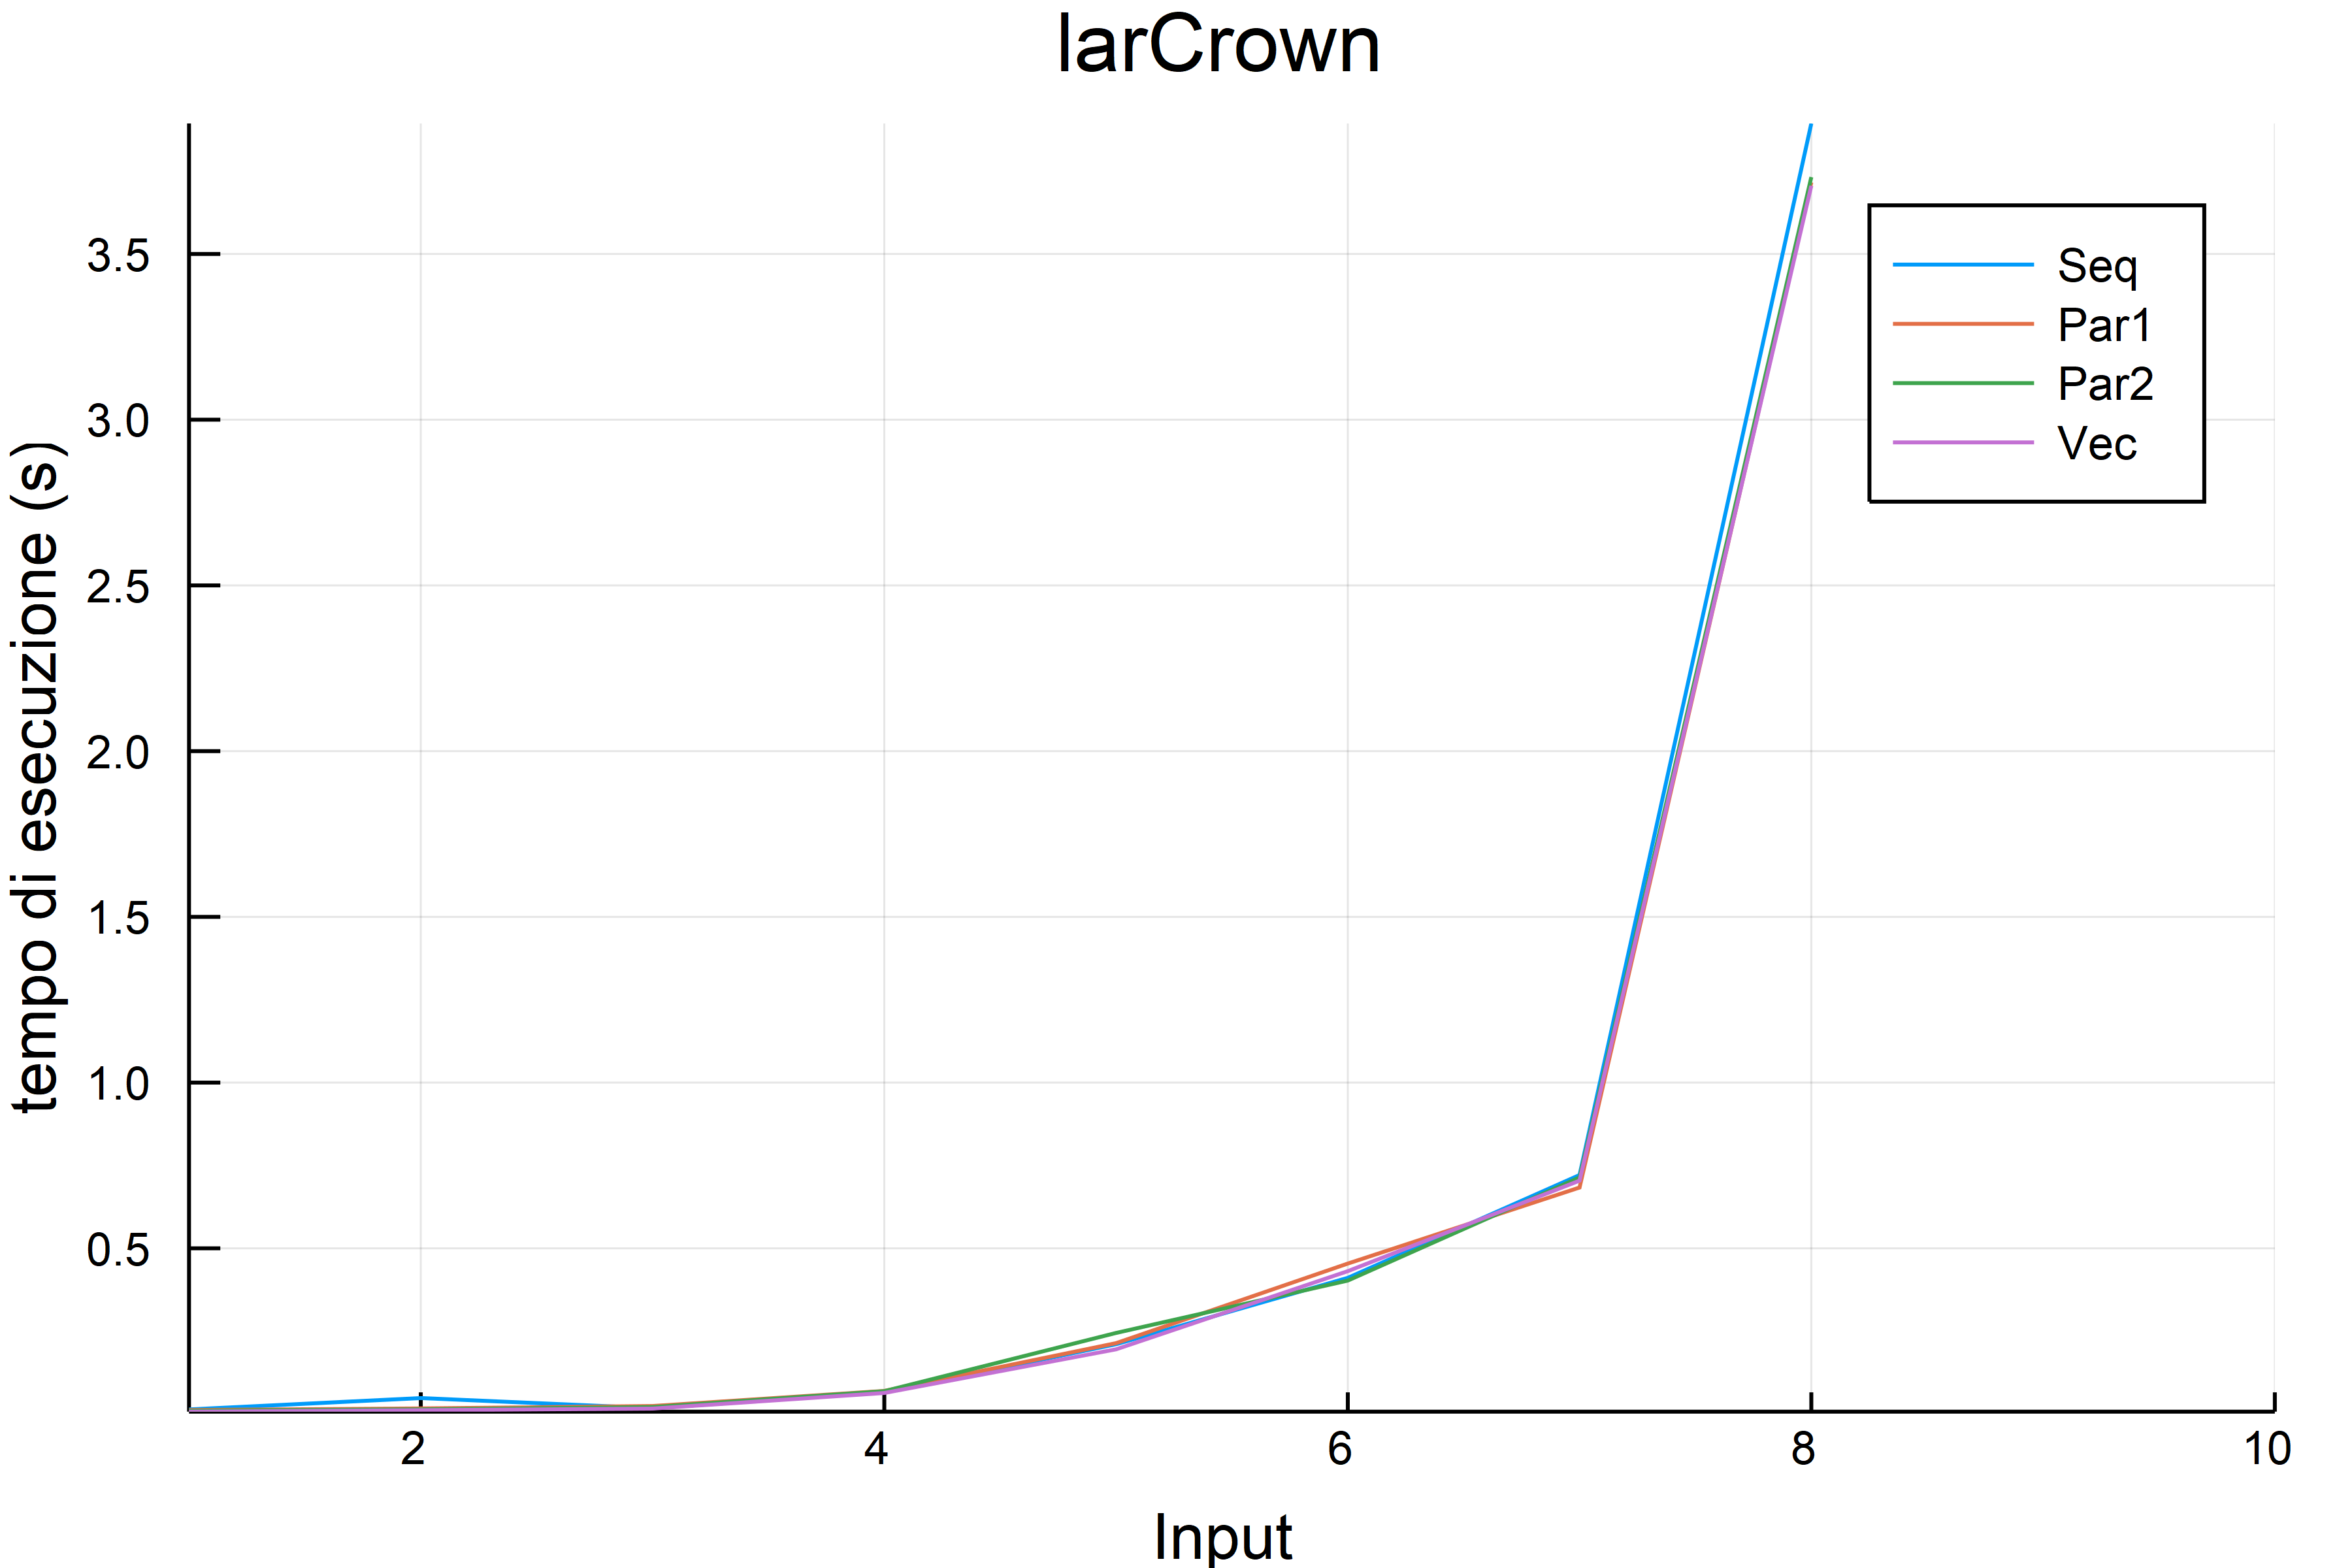
\includegraphics[scale=.13]{larCrownTime.png} 
\caption{Results computed on Microsoft Surface Pro  3 (4GB LPDDR3 1600 MHz RAM, i5-4300U processor)} 
\end{figure}
%---------------------------------------------------------------------------------
\subsection{larBox}

\paragraph{Python}

\begin{verbatim}
def larBox(minVect,maxVect):
    size = VECTDIFF([maxVect,minVect])#2
    print "size =",size
    box = larApply(s(*size))(larCuboids([1]*len(size)))
    print "box =",box
    return larApply(t(*minVect))(box)
\end{verbatim}

\paragraph{Julia}

\begin{verbatim}
function larBox(minVect,maxVect)
    siz = maxVect-minVect
    box = larApplyMapper(s(siz))(LARLIB.larCuboids(fill(1,length(siz))))
    return larApplyMapper(t(minVect))(box)
end 
\end{verbatim}

The \textfb{larBox} function creates a rectangle parallelepiped with given extremes ($minVect$ and $maxVect$).

With $$\verb!siz=maxVect-minVect!$$ an array subtraction is performed, subtracting component by component.

With $$\verb!length(siz)!$$ we calculate the length of the difference vector found in the previous step.

With $$\verb!fill(1,length(siz))!$$ we generate a vector containing a number of $1$ equal to \verb!d=length(siz)!.

LARLIB.larCuboids is applied to the array, generating a cuboidal complex in the form $[1,...,1]$.

\verb!s(siz)! generates a square matrix of size $d+1$ such that the elements on the diagonal of the submatrix $d*d$ are the elements of \verb!siz!, while the element $d+1$ on the diagonal is 1.0. Every other element outside of the diagonal is null.

\paragraph{Visualization examples}

\begin{verbatim}
V,CV = larBox([-1,-1,-1],[1,1,1])
V
CV=CV-1
W = [Any[V[h,k] for h=1:size(V,1)] for k=1:size(V,2)]
hpc = p.STRUCT(p.MKPOLS(PyObject([W,CV,[]])))
p.VIEW(hpc)
\end{verbatim}

\begin{figure}[htbp] 
\centering 
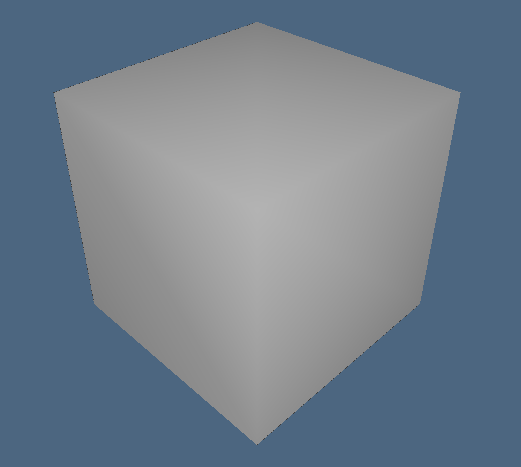
\includegraphics[scale=.35]{larBox.png} 
\caption{Unit cube.} 
\end{figure}

\paragraph{Test}
\begin{Verbatim}
@testset "larBox" begin
	@test BoxCalculation(larBox([-1,-1,-1],[1,1,1])[1])==(1+1)^3
	@test BoxCalculation(larBox([-1,-1],[1,1])[1])==4
	@test BoxCalculation(larBox([-1,0,-3],[1,4,5])[1])==(1+1)*(4+0)*(5+3)
	@test BoxCalculation(larBox([2,3],[4,5])[1])==(4-2)*(5-3)
	#(y1-x1)*(y2-x2)*(y3-x3)
end
\end{Verbatim}

\paragraph{Vectorization}

\begin{Verbatim}
function flarBoxV(siz::Array,minVect::Array)
    function f0(V::Array)
        return [siz[i]*V[i]+minVect[i] for i in 1:length(V)]
    end
    return f0
end

function larBoxV(minVect,maxVect)
    siz = maxVect-minVect
    V,CV = LARLIB.larCuboids(fill(1,length(siz)))
    V = [V[:,k] for k=1:size(V,2)]
    W = hcat(flarBoxV(siz,minVect).(V)...)
    return W,CV
end
\end{Verbatim}

\paragraph{Parallel Computing}
\begin{Verbatim}
function larBoxP(minVect,maxVect)
    siz = maxVect-minVect
    V,CV = LARLIB.larCuboids(fill(1,length(siz)))
    V = SharedArray(V)
    W = SharedArray{Float64}(length(siz),size(V,2))
    @sync @parallel for i = 1:length(siz)
        @sync @parallel for j = 1:size(V,2)
            W[i,j] = siz[i]*V[i,j]+minVect[i]
        end
    end
    return W,CV
end
\end{Verbatim}

\begin{Verbatim}
@testset "Vectorized and Parallelized larBox" begin
	@test BoxCalculation(larBoxV([-1,-1,-1],[1,1,1])[1])==(1+1)^3
	@test BoxCalculation(larBoxP([-1,-1],[1,1])[1])==4
	@test BoxCalculation(larBoxV([-1,0,-3],[1,4,5])[1])==(1+1)*(4+0)*(5+3)
	@test BoxCalculation(larBoxP([2,3],[4,5])[1])==(4-2)*(5-3)
end
\end{Verbatim}

\paragraph{Performance evaluation\\}

In this case Time Calculate has been changed because larBox has two arguments.

\begin{Verbatim}

function TimeCalculateLBox(f::Function,arg1,arg2,n::Int64)
    f(arg1,arg2);
    t = Array{Float64}(n)
    for i = 1:n
        t[i] = @elapsed f(arg1,arg2)
    end
    m = mean(t)
    return m
end

x = 1:20
yS = [TimeCalculateLBox(larBox,rand(Int,m),rand(Int,m),5) for m in x]
yP = [TimeCalculateLBox(larBoxP,rand(Int,m),rand(Int,m),5) for m in x]
yV = [TimeCalculateLBox(larBoxV,rand(Int,m),rand(Int,m),5) for m in x]
y = hcat(yS,yP,yV)
plot(x,y,yaxis=("tempo di esecuzione (s)"),xaxis=("Input",(1,25)),
label=["Seq" "Par" "Vect"],title="larBox",lw=1)

\end{Verbatim}

\begin{figure}[htbp] 
\centering 
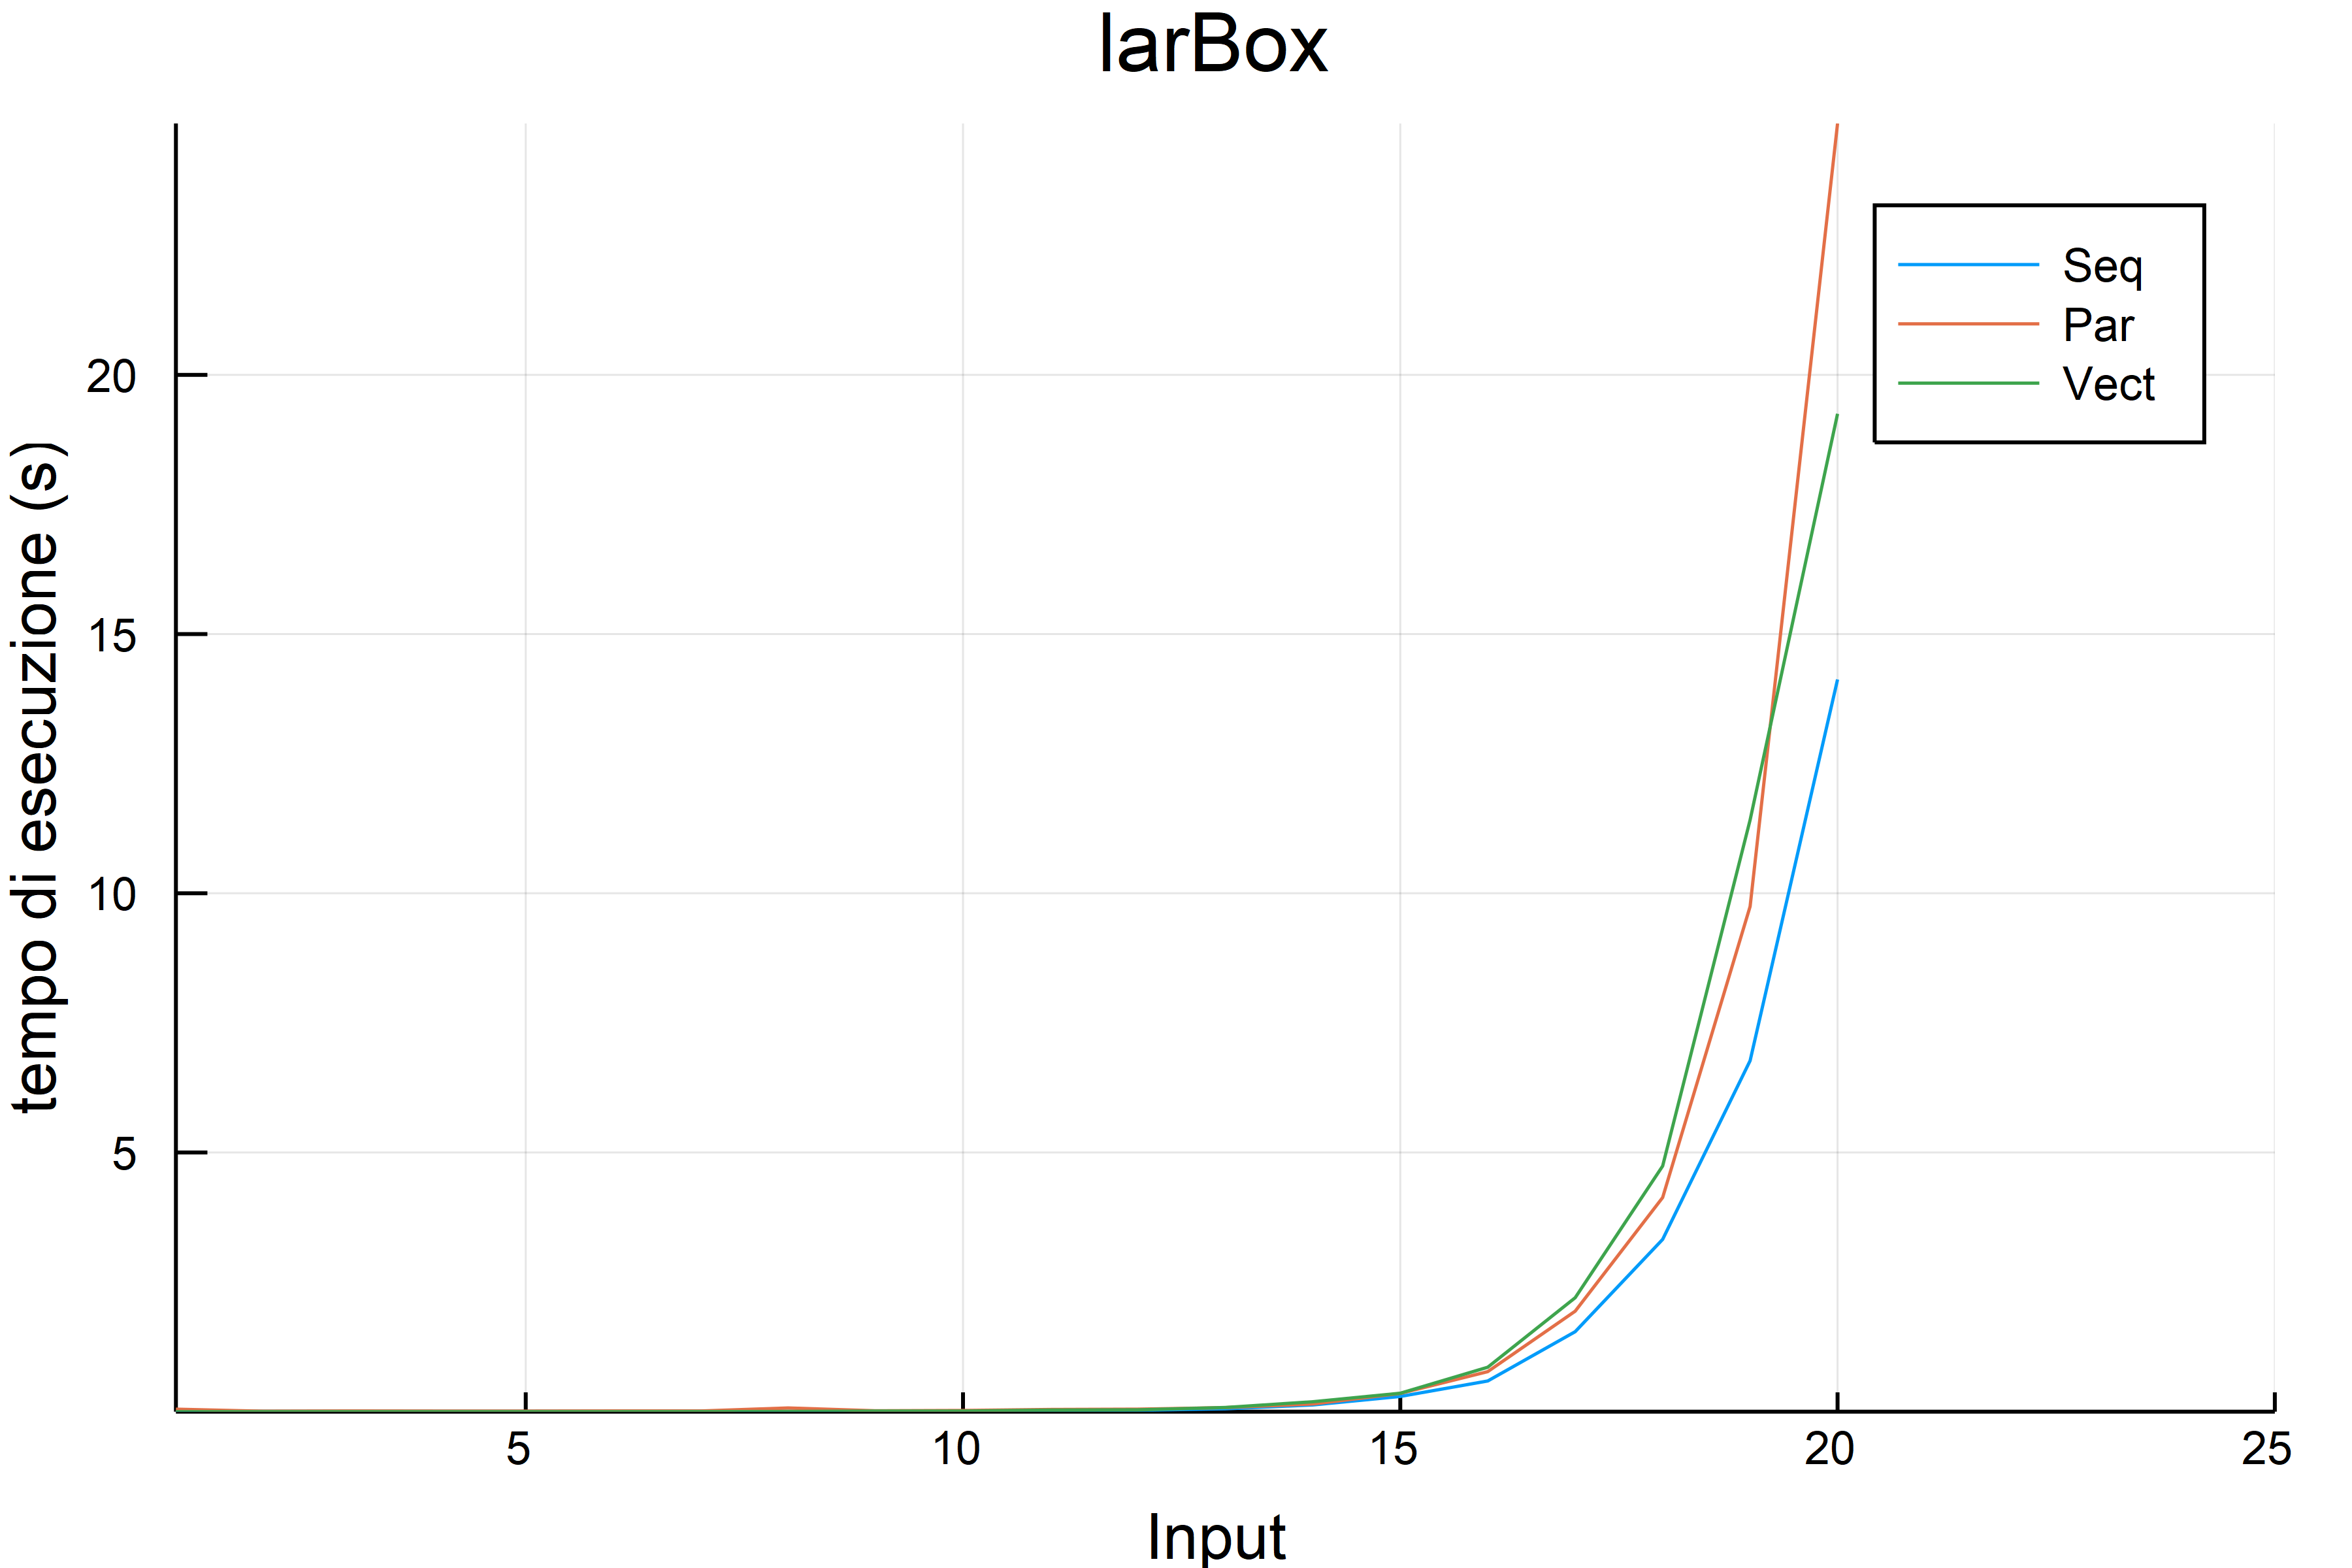
\includegraphics[scale=.13]{larBoxTime.png} 
\caption{Results computed on Microsoft Surface Pro  3 (4GB LPDDR3 1600 MHz RAM, i5-4300U processor)} 
\end{figure}
%---------------------------------------------------------------------------------
\subsection{larBall}

\paragraph{Python}

\begin{verbatim}
def larBall(radius=1,angle1=PI,angle2=2*PI):
    def larBall0(shape=[18,36]):
        V,CV = checkModel(larSphere(radius,angle1,angle2)(shape))
        return V,[range(len(V))]
    return larBall0
\end{verbatim}

\paragraph{Julia}

\begin{verbatim}
function larBall(radius=1,angle1=pi,angle2=2*pi)
    function larBall0(shape=[18,36])
        V,CV = larSphere(radius,angle1,angle2)(shape)
        W = [Any[V[h,k] for h=1:size(V,1)] for k=1:size(V,2)]
        W = [map(approxVal(4),v) for v in W]
        X = hcat(collect(Set(W))...)
        return X,[collect(0:size(X,2)-1)]
    end
    return larBall0
end
\end{verbatim}

The \textfb{larBall} function creates a sphere centered in the origin with given radius and angles.

The model to "fill" is generated with $$\verb!V,CV = larSphere(radius,angle1,angle2)(shape)!$$. In this case, a spherical surface.

With $$\verb!W = [Any[V[h,k] for h = 1:size(V,1)] for k = 1:size(V,2)]!$$ as opposed to $hcat$, we dispose the coordinates of the vertices (i.e. the columns in V) horizontally (into an array of arrays).  

With $$\verb!W = [map(approxVal(4),v) for v in W]!$$ we round every element of each array in W to the fourth decimal place.

\verb!Set(W)! deletes the doubles in W and saves them in a set, with $collect$ this collection is turned back into an array of arrays: the elements are the coordinates of the sphere vertices.
With the $hcat$ function the coordinates of the vertices just created are arranged vertically in a matrix.

Named \verb!n=size(X, 2)! the number of columns in X, then the function returns the matrix X of the vertices and the array $[0,1,2,3,...,n-1]$.

\paragraph{Visualization examples}

\begin{verbatim}
V,CV = larBall(1,pi,pi)()
V
CV
W = [Any[V[h,k] for h=1:size(V,1)] for k=1:size(V,2)]
hpc = p.STRUCT(p.MKPOLS(PyObject([W,CV,[]])))
p.VIEW(hpc)
\end{verbatim}

\begin{figure}[htbp] 
\centering 
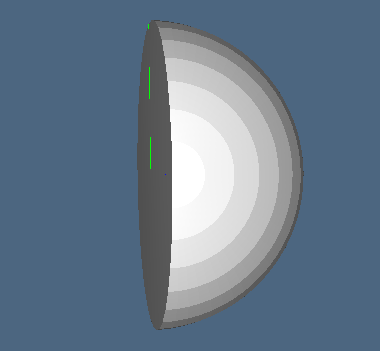
\includegraphics[scale=.49]{larBall.png} 
\caption{Section of the unit radius sphere centered in the origin.} 
\end{figure}

\paragraph{Test}
\begin{Verbatim}
@testset "larBall" begin
	@test BoxCalculation(larBall(1,pi,2*pi)()[1])==8
	@test BoxCalculation(larBall(6,pi,pi)()[1])==864
	@test BoxCalculation(larBall(3,pi,2*pi)()[1])==6^3
	#(radius*2)^3
	@test size(larBall(2.6,pi/5,pi/9)()[1],2)==703
	@test length(larBall(2.6,pi/5,pi/9)()[2])==1
end
\end{Verbatim}

\paragraph{Vectorization\\}

\begin{Verbatim}
function larBallV(radius=1,angle1=pi,angle2=2*pi)
    function larBall0(shape=[18,36])
        V = larSphere(radius,angle1,angle2)(shape)[1]
        V = approxVal(4).(V)
        W = hcat(collect(Set([V[:,k] for k=1:size(V,2)]))...)
        return W,[collect(0:size(W,2)-1)]
    end
    return larBall0
end
\end{Verbatim}

\paragraph{Parallel Computing\\}

\begin{Verbatim}
function larBallP(radius=1,angle1=pi,angle2=2*pi)
    function larBall0(shape=[18,36])
        V = larSphereP(radius,angle1,angle2)(shape)[1]
        V = SharedArray(V)
        @sync @parallel for i = 1:size(V,2)
            V[1,i] = approxVal(4)(V[1,i])
            V[2,i] = approxVal(4)(V[2,i])
            V[3,i] = approxVal(4)(V[3,i])
        end
        W = hcat(collect(Set([V[:,k] for k=1:size(V,2)]))...)
        return W,[collect(0:size(W,2)-1)]
    end
    return larBall0
end
\end{Verbatim}

\begin{Verbatim}
@everywhere function fP(SV::SharedArray,indexprt,ultim)
    id = myid()
    if id != nprocs()
        for i=indexprt*(id-2) +1 : indexprt*(id-1)
            SV[1,i] = approxVal(4)(SV[1,i])
            SV[2,i] = approxVal(4)(SV[2,i])
            SV[3,i] = approxVal(4)(SV[3,i])
        end
    else
        for i=indexprt*(id-2) +1 : ultim
            SV[1,i] = approxVal(4)(SV[1,i])
            SV[2,i] = approxVal(4)(SV[2,i])
            SV[3,i] = approxVal(4)(SV[3,i])
        end
    end
end

function larBallPP(radius=1,angle1=pi,angle2=2*pi)
    function larBall0(shape=[18,36])
        V = larSphereP(radius,angle1,angle2)(shape)[1]
        V = SharedArray(V)
        if nprocs() > size(V,2)
            indexprt = 1
        else
            indexprt = Int((size(V,2)-(size(V,2)%nprocs()))/nprocs())
        end
        @sync begin
            for i = 2:nprocs()
                @async remotecall_fetch(fP,i,V,indexprt,size(V,2))
            end
        end
        W = hcat(collect(Set([V[:,k] for k=1:size(V,2)]))...)
        return W,[collect(0:size(W,2)-1)]
    end
    return larBall0
end
\end{Verbatim}

\begin{Verbatim}
@testset "Vectorized and Parallelized larBall" begin
	@test BoxCalculation(larBallV(1,pi,2*pi)()[1])==8
	@test BoxCalculation(larBallP(6,pi,pi)()[1])==864
	@test BoxCalculation(larBallPP(3,pi,2*pi)()[1])==6^3
	@test BoxCalculation(larBallP(1,pi,2*pi)()[1])==8
	@test BoxCalculation(larBallPP(6,pi,pi)()[1])==864
	@test BoxCalculation(larBallV(3,pi,2*pi)()[1])==6^3
end
\end{Verbatim}

\paragraph{Performance evaluation}

\begin{Verbatim}
data = [[x,1] for x in data3]

x,y = TimeGraph(larBall(),larBallP(),larBallPP(),larBallV(),data,5)
plot(x,y,yaxis=("tempo di esecuzione (s)"),xaxis=("Input",(1,length(x)+2)),
label=["Seq" "Par1" "Par2" "Vec"],title="larBall",lw=1)

\end{Verbatim}

\begin{figure}[htbp] 
\centering 
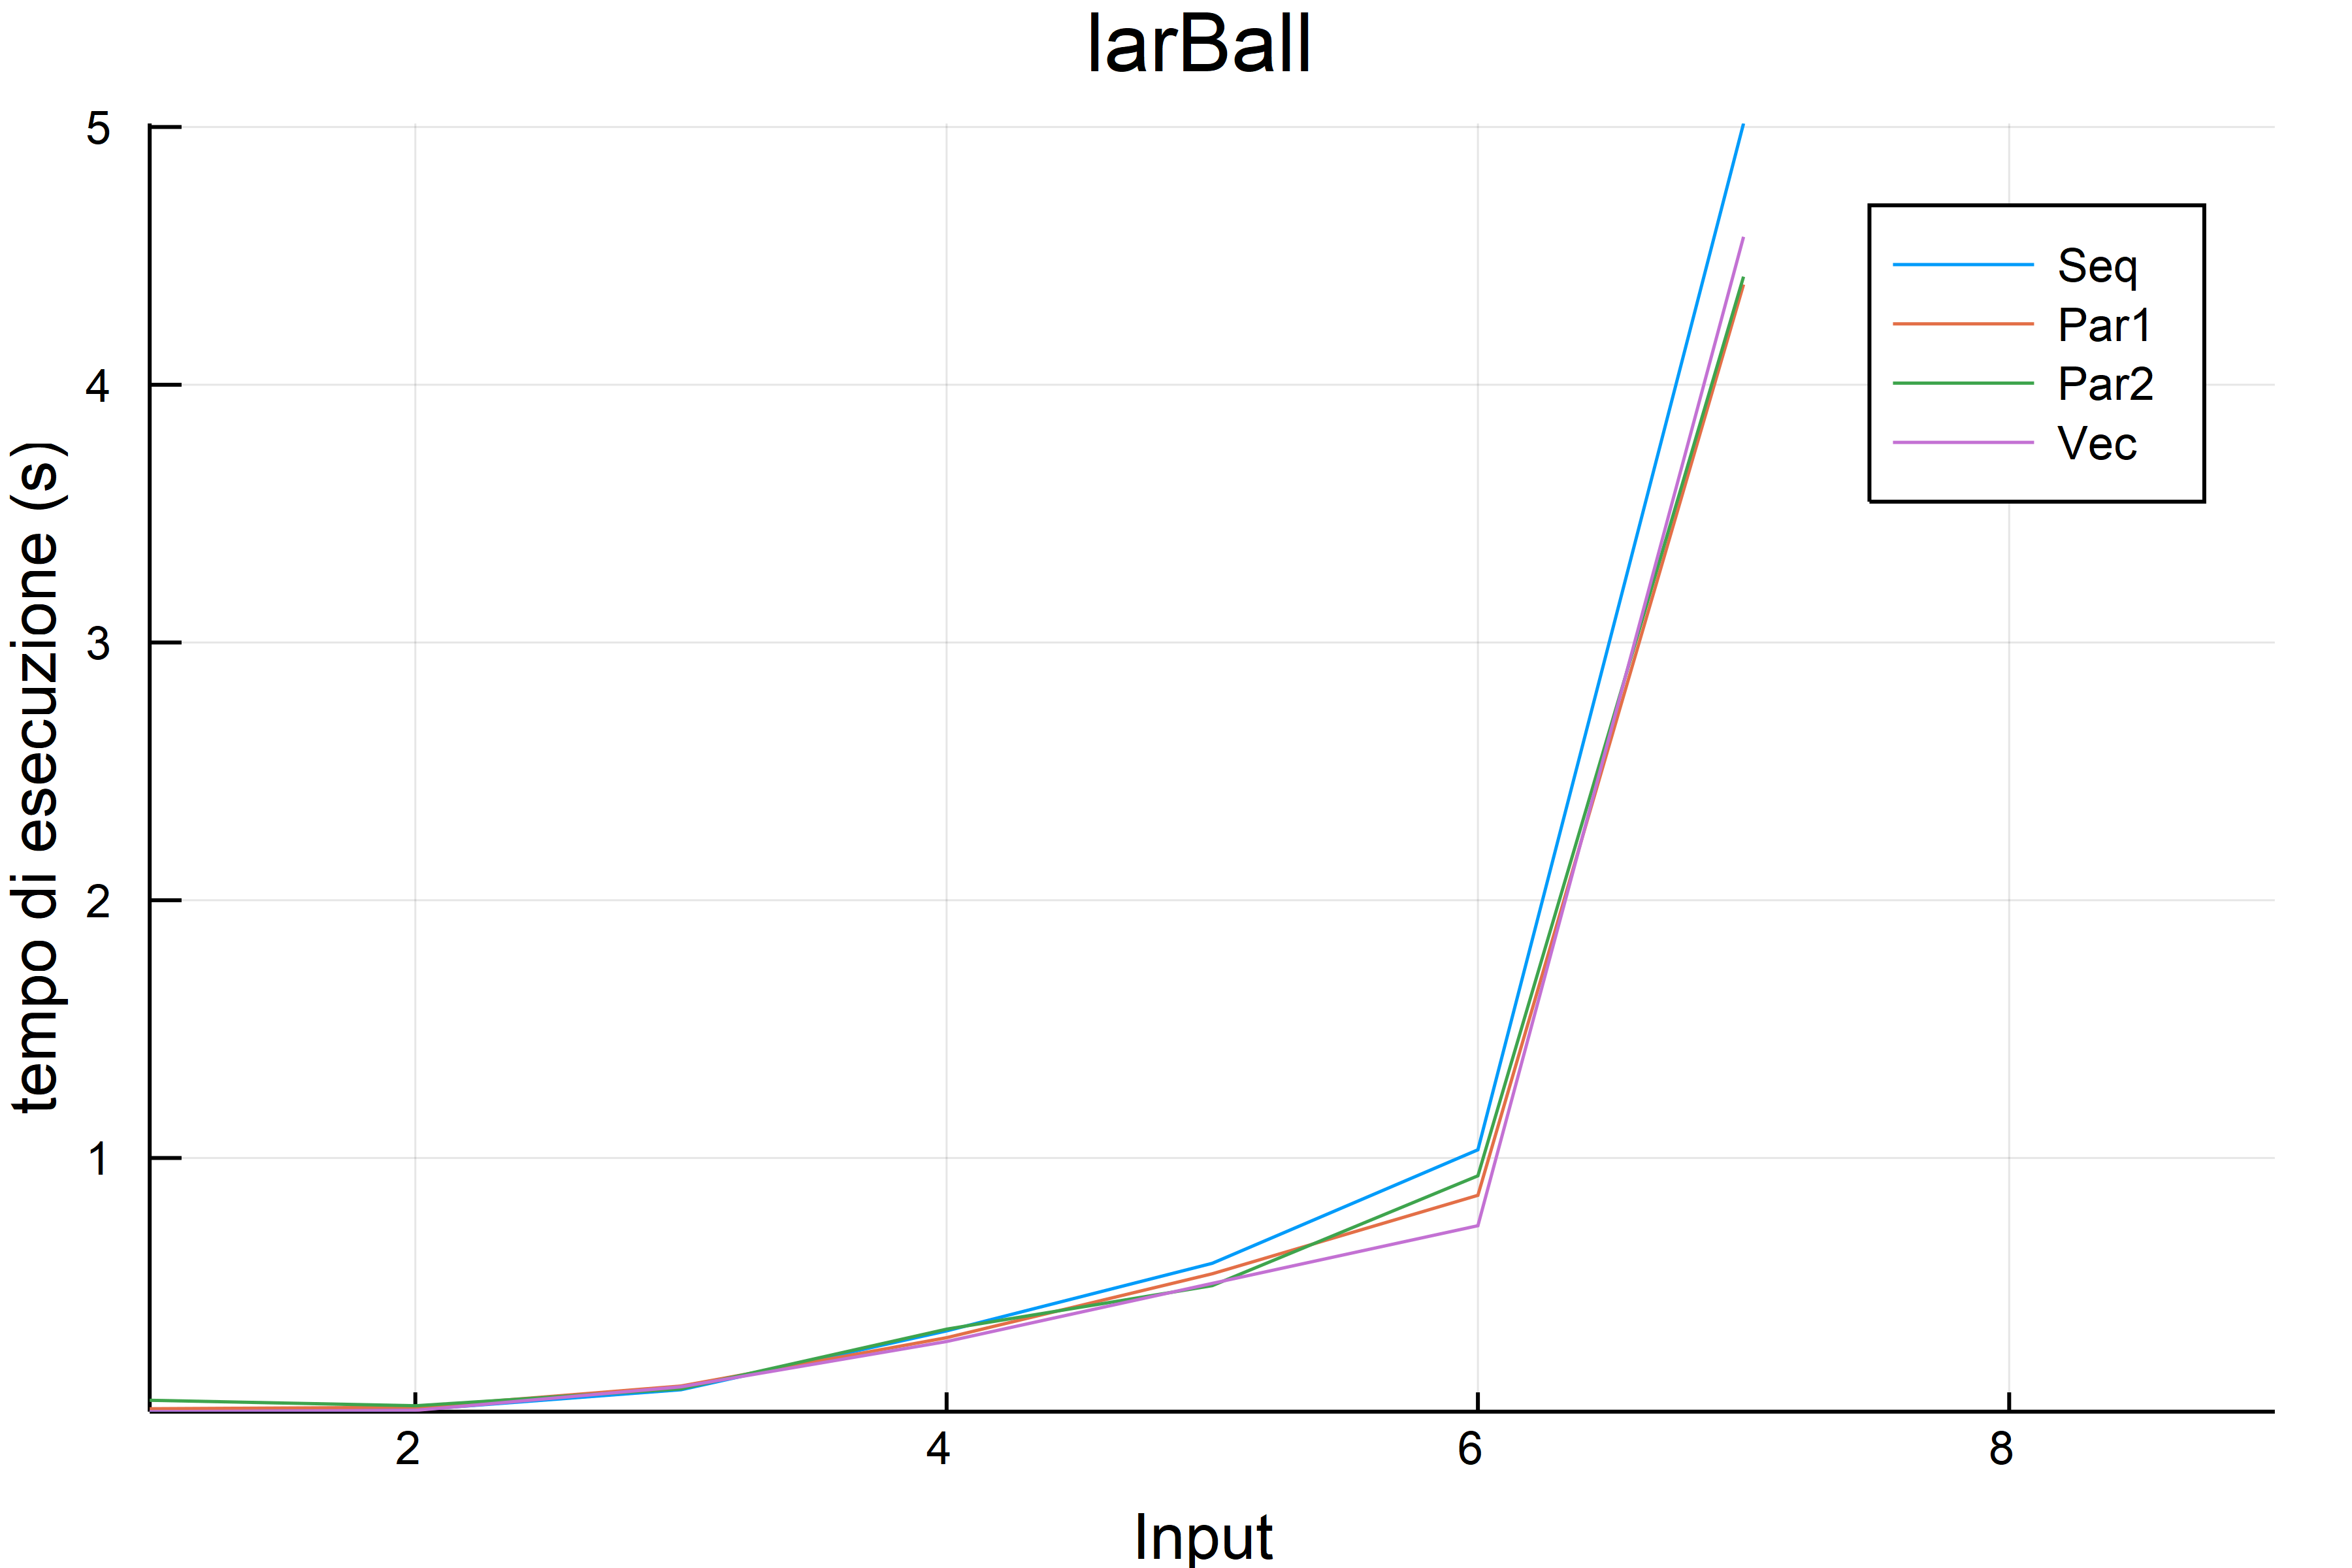
\includegraphics[scale=.13]{larBallTime.png} 
\caption{Results computed on Microsoft Surface Pro  3 (4GB LPDDR3 1600 MHz RAM, i5-4300U processor)} 
\end{figure}

%---------------------------------------------------------------------------------
\subsection{larRod}

\paragraph{Python}

\begin{verbatim}
def larRod(radius,height,angle=2*PI):
    def larRod0(shape=[36,1]):
        V,CV = checkModel(larCylinder(radius,height,angle)(shape))
        return V,[range(len(V))]
    return larRod0	
\end{verbatim}

\paragraph{Julia}

\begin{verbatim}
function larRod(radius=1,height=3,angle=2*pi)
    function larRod0(shape=[36,1])
        V,CV = larCylinder(radius,height,angle)(shape)
        W = [Any[V[h,k] for h=1:size(V,1)] for k=1:size(V,2)]
        W = [map(approxVal(4),v) for v in W]
        X = hcat(collect(Set(W))...)
        return X,[collect(0:size(X,2)-1)]
    end
    return larRod0
end
\end{verbatim}

The \textfb{larRod} function creates a solid rod centered in the origin of given radius, height and angle.

The model to "fill" is generated with $$\verb!V,CV = larCylinder(radius,height,angle)(shape)!$$ in this case a cylinder. 

With $$\verb!W = [Any[V[h,k] for h = 1:size(V,1)] for k = 1:size(V,2)]!,$$ as opposed to $hcat$, we dispose the coordinates of the vertices (i.e. the columns in V) horizontally (into an array of arrays).

With $$\verb!W = [map(approxVal(4),v) for v in W]!$$ we round every element of each array in W to the fourth decimal place.

\verb!Set(W)! deletes the doubles contained in W and saves them in a set, with $collect$ this collection is turned back into an array of arrays: the elements are the coordinates of the cylinder.
With the $hcat$ function the coordinates of the vertices just created are arranged vertically in a matrix.

Named \verb!n=size(X,2)! the number of columns in X, then the function returns the vertices matrix X and the array $[0,1,2,3,...,n-1]$.

\paragraph{Visualization examples}

\begin{verbatim}
V,CV = larRod()()
V
CV
W = [Any[V[h,k] for h=1:size(V,1)] for k=1:size(V,2)]
hpc = p.STRUCT(p.MKPOLS(PyObject([W,CV,[]])))
p.VIEW(hpc)
\end{verbatim}

\begin{figure}[htbp] 
\centering 
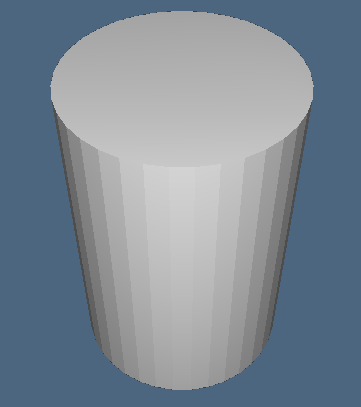
\includegraphics[scale=.45]{larRod.png} 
\caption{Unit radius solid cylinder centered in the origin of height 3.} 
\end{figure}

\paragraph{Test}

\begin{Verbatim}
@testset "larRod" begin
	@test BoxCalculation(larRod(1,5,2*pi)()[1])==20
	@test BoxCalculation(larRod(2,2,pi)()[1])==16
	@test BoxCalculation(larRod(1,4,pi)()[1])==8
	#((radius*2)^2)*height
	@test size(larRod(3.7,8.9,pi/9)()[1],2)==74
	@test length(larRod(3.7,8.9,pi/9)()[2])==1
end
\end{Verbatim}

\paragraph{Vectorization\\}
\begin{Verbatim}
function larRodV(radius=1,height=3,angle=2*pi)
    function larRod0(shape=[36,1])
        V,CV = larCylinder(radius,height,angle)(shape)
        V = approxVal(4).(V)
        W = hcat(collect(Set([V[:,k] for k=1:size(V,2)]))...)
        return W,[collect(0:size(W,2)-1)]
    end
    return larRod0
end
\end{Verbatim}

\paragraph{Parallel Computing\\}

\begin{Verbatim}
function larRodP(radius=1,height=3,angle=2*pi)
    function larRod0(shape=[36,1])
        V,CV=larCylinderP(radius,height,angle)(shape)
        V = SharedArray(V)
        @sync @parallel for i = 1:size(V,2)
            V[1,i] = approxVal(4)(V[1,i])
            V[2,i] = approxVal(4)(V[2,i])
            V[3,i] = approxVal(4)(V[3,i])
        end
        W = hcat(collect(Set([V[:,k] for k=1:size(V,2)]))...)
        return W,[collect(0:size(W,2)-1)]
    end
    return larRod0
end
\end{Verbatim}

\begin{Verbatim}
function larRodPP(radius=1,height=3,angle=2*pi)
    function larRod0(shape=[36,1])
        V,CV=larCylinderP(radius,height,angle)(shape)
        V = SharedArray(V)
        if nprocs() > size(V,2)
            indexprt = 1
        else
            indexprt = Int((size(V,2)-(size(V,2)%nprocs()))/nprocs())
        end
        @sync begin
            for i = 2:nprocs()
                @async remotecall_fetch(fP,i,V,indexprt,size(V,2))
            end
        end
        W = hcat(collect(Set([V[:,k] for k=1:size(V,2)]))...)
        return W,[collect(0:size(W,2)-1)]
    end
    return larRod0
end
\end{Verbatim}

\begin{Verbatim}
@testset "Vectorized and Parallelized larRod" begin
	@test BoxCalculation(larRodV(1,5,2*pi)([56,1])[1])==20
	@test BoxCalculation(larRodP(2,2,pi)([56,1])[1])==16
	@test BoxCalculation(larRodPP(1,4,pi)([56,1])[1])==8
	@test BoxCalculation(larRodP(1,5,2*pi)([56,1])[1])==20
	@test BoxCalculation(larRodPP(2,2,pi)([56,1])[1])==16
	@test BoxCalculation(larRodV(1,4,pi)([56,1])[1])==8
end
\end{Verbatim}

\paragraph{Performance evaluation}

\begin{Verbatim}
data = [[x,1] for x in data2]

x,y = TimeGraph(larRod(),larRodP(),larRodPP(),larRodV(),data,5)
plot(x,y,yaxis=("tempo di esecuzione (s)"),xaxis=("Input",(1,length(x)+2)),
label=["Seq" "Par1" "Par2" "Vec"],title="larRod",lw=1)

\end{Verbatim}

\begin{figure}[htbp] 
\centering 
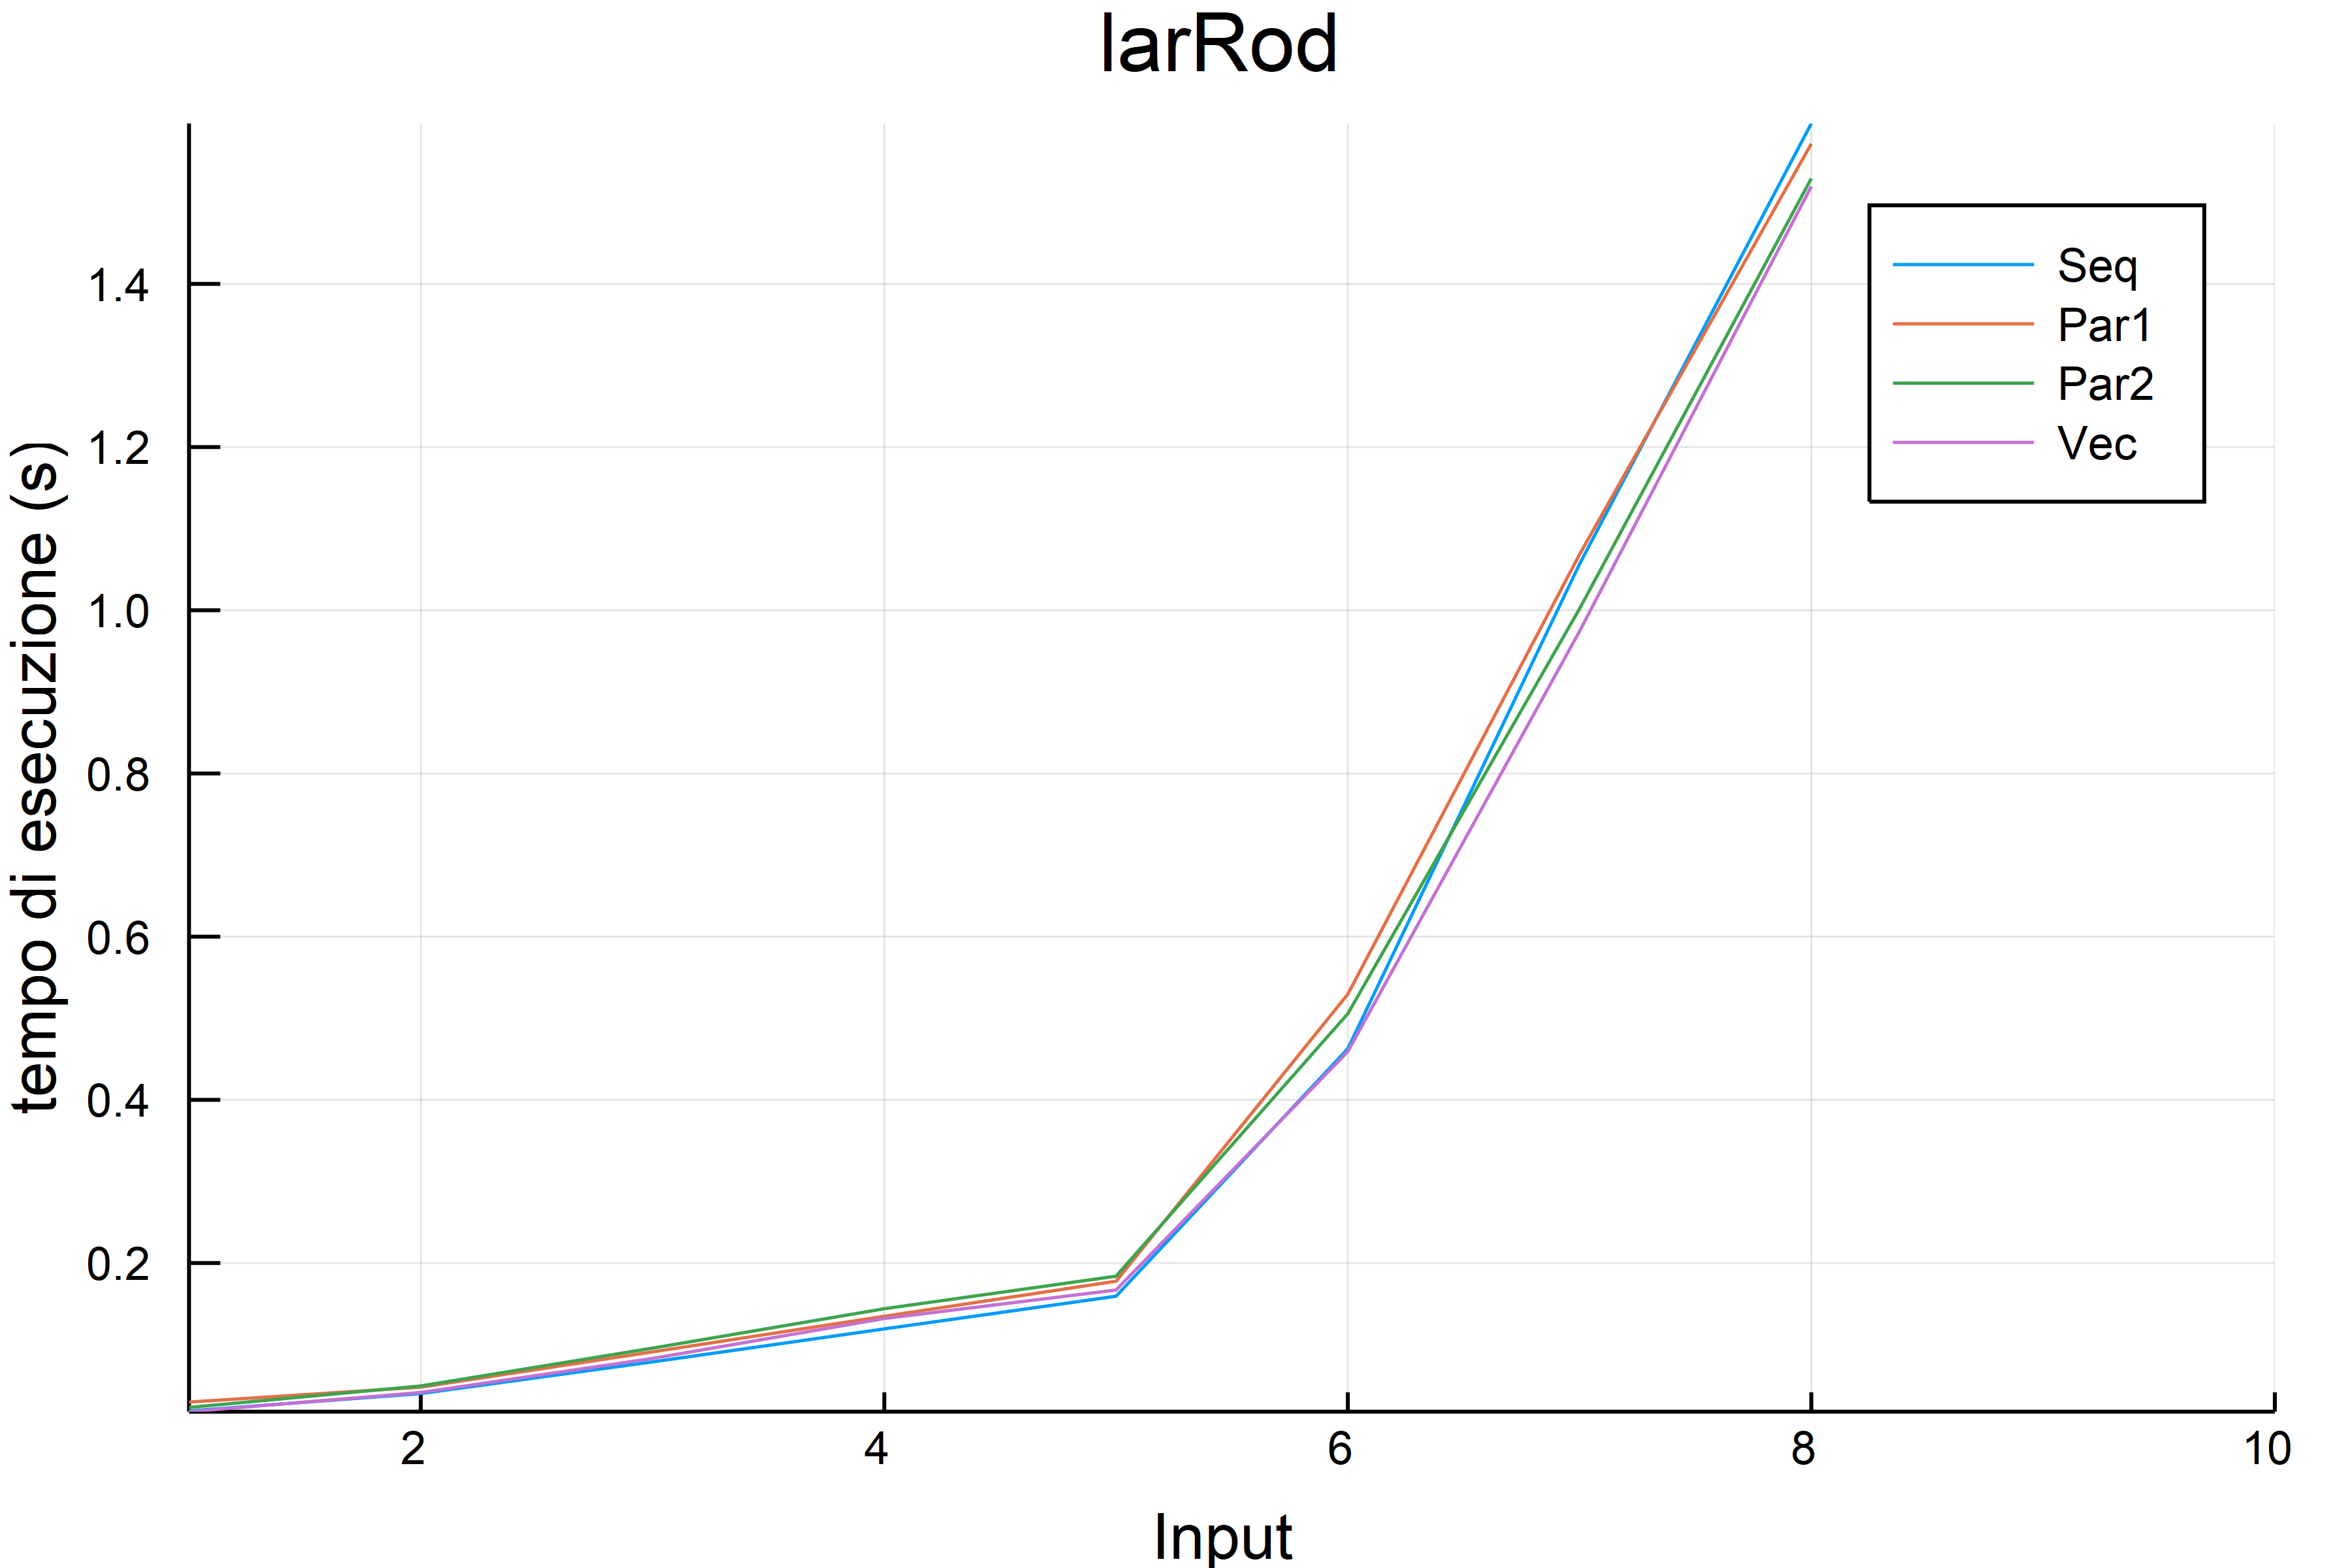
\includegraphics[scale=.13]{larRodTime.png} 
\caption{Results computed on Microsoft Surface Pro  3 (4GB LPDDR3 1600 MHz RAM, i5-4300U processor)} 
\end{figure}
%---------------------------------------------------------------------------------
\subsection{larHollowCyl}

\paragraph{Python}

\begin{verbatim}
def larHollowCyl(r,R,height,angle=2*PI):
    def larHollowCyl0(shape=[36,1,1]):
        V,CV = larIntervals(shape)([angle,R-r,height])
        V = larTranslate([0,r,0])(V)
        domain = V,CV
        x = lambda p : p[1] * COS(p[0])
        y = lambda p : p[1] * SIN(p[0])
        z = lambda p : p[2] * height
        return larMap([x,y,z])(domain)
    return larHollowCyl0
\end{verbatim}

\paragraph{Julia}

\begin{verbatim}
function larHollowCyl(r,R,height,angle=2*pi)
    function larHollowCyl0(shape=[36,1,1])
        V,CV = LARLIB.larCuboids(shape)
        V = [angle/shape[1] 0 0;0 (R-r)/shape[2] 0;0 0 height/shape[3]]*V
        V = broadcast(+,V,[0,r,0])
        W = [V[:,k] for k=1:size(V,2)]
        X = hcat(map(p->let(u,v,z)=p;[v*cos(u);v*sin(u);z] end,W)...)
        return X,CV
    end
    return larHollowCyl0
end
\end{verbatim}

The \textfb{larHollowCyl} function creates an hollow cylinder with given radiuses, height and angle.

In this case, the local parametrization used is:
$$f(u,v,z)=(vcos(u);vsin(u);z),$$
with $[u,v,z] \in [0,angle]\times[r,R]\times[0,height]$.

With $$\verb!V=broadcast(+,V,[0,r,0])!$$ we sum 0 to each element in the first row of V, r to each element in the second row of V and 0 to every element in the third row of V.

With $$\verb!W=[V[:,k] for k=1:size(V,2)]!,$$ as opposed to $hcat$, we dispose the coordinates of the vertices (i.e. the columns in V) horizontally (into an array of arrays).

Then $map$ applies the "anonymous function" $$\verb!p->let(u,v)=p[radius*cos(u)*cos(v);radius*cos(u)*sin(v);radius*sin(u)]end!$$ to the coordinates of all the vertices contained in the W collection. Next, with the $hcat$ function, the coordinates of the new vertices are rearranged vertically in a matrix.

\paragraph{Visualization examples}

\begin{verbatim}
V,CV = larHollowCyl(1,2,4,pi)([36,1,1])
V
CV
V = hcat(V[:,1],[V[:,k] for k in 1:size(V,2)]...)
W = [Any[V[h,k] for h=1:size(V,1)] for k=1:size(V,2)]
hpc = p.STRUCT(p.MKPOLS(PyObject([W,CV,[]])))
p.VIEW(hpc)
\end{verbatim}

\begin{figure}[htbp] 
\centering 
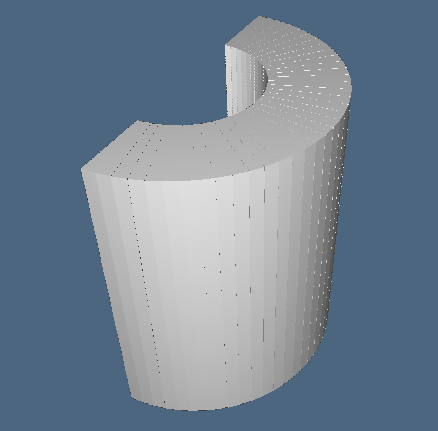
\includegraphics[scale=.39]{larHollowCyl.png} 
\caption{Half hollow cylinder centered in the origin of height 4 and radiuses 1 and 2.} 
\end{figure}

\paragraph{Test}
\begin{Verbatim}
@testset "larHollowCyl" begin
	@test BoxCalculation(larHollowCyl(0,1,5,2*pi)()[1])==20
	@test BoxCalculation(larHollowCyl(1,2,4,pi)()[1])==32
	@test BoxCalculation(larHollowCyl(1,4,3,pi/2)()[1])==48
	#((radius*2)^2)*height
	@test size(larHollowCyl(3.4,7.8,pi/5)()[1],2)==148
	@test length(larHollowCyl(3.4,7.8,pi/5)()[2])==36
end
\end{Verbatim}

\paragraph{Vectorization}

\begin{verbatim}
function larHollowCylV(r,R,height,angle=2*pi)
	function larHollowCyl0(shape=[36,1,1])
		V,CV=LARLIB.larCuboids(shape)
		V = [V[:,k] for k=1:size(V,2)]
		W = (p->[p[2]*cos(p[1]),p[2]*sin(p[1]),p[3]]).((x->[x[1]*angle/shape[1],
		    x[2]*(R-r)/shape[2]+r, x[3]*height/shape[3]]).(V))
        return hcat(W...),CV
    end
    return larHollowCyl0
end
\end{verbatim}

\paragraph{Parallel Computing}
\begin{Verbatim}
function larHollowCylP(r,R,height,angle=2*pi)
    function larHollowCyl0(shape=[36,1,1])
        V,CV = LARLIB.larCuboids(shape)
        V = SharedArray(V)
        W = SharedArray{Float64}(3,size(V,2))           
        @sync @parallel for i = 1:size(V,2)         
            W[1,i] = (V[2,i]*(R-r)/shape[2]+r)*cos(V[1,i]*angle/shape[1])           
            W[2,i] = (V[2,i]*(R-r)/shape[2]+r)*sin(V[1,i]*angle/shape[1])
            W[3,i] = V[3,i]*height/shape[3]
        end
        return W,CV
    end
    return larHollowCyl0
end
\end{Verbatim}

\begin{Verbatim}
@everywhere function flarHollowCyl(W::SharedArray,V::Array,indexprt,ultim,
            shape,r,R,height,angle)
    id = myid()
    if id != nprocs()
        for i=indexprt*(id-2) +1 : indexprt*(id-1)
            W[1,i] = (V[2,i]*(R-r)/shape[2]+r)*cos(V[1,i]*angle/shape[1])           
            W[2,i] = (V[2,i]*(R-r)/shape[2]+r)*sin(V[1,i]*angle/shape[1])
            W[3,i] = V[3,i]*height/shape[3]
        end
    else
        for i=indexprt*(id-2) +1 : ultim
            W[1,i] = (V[2,i]*(R-r)/shape[2]+r)*cos(V[1,i]*angle/shape[1])           
            W[2,i] = (V[2,i]*(R-r)/shape[2]+r)*sin(V[1,i]*angle/shape[1])
            W[3,i] = V[3,i]*height/shape[3]
        end
    end
end

function larHollowCylPP(r,R,height,angle=2*pi)
    function larHollowCyl0(shape=[36,1,1])
        V,CV = LARLIB.larCuboids(shape)
        W = SharedArray{Float64}(3,size(V,2))           
        if nprocs() > size(V,2)
            indexprt = 1
        else
            indexprt = Int((size(V,2)-(size(V,2)%nprocs()))/nprocs())
        end
        @sync begin
            for i = 2:nprocs()
                @async remotecall_fetch(flarHollowCyl,i,W,V,indexprt,size(V,2),
                shape,r,R,height,angle)
            end
        end
        return W,CV
    end
    return larHollowCyl0
end
\end{Verbatim}

\begin{Verbatim}
@testset "Vectorized and Parallelized larHollowCyl" begin
    @test BoxCalculation(larHollowCylV(0,1,5,2*pi)()[1])==20
    @test BoxCalculation(larHollowCylP(1,2,4,pi)()[1])==32
    @test BoxCalculation(larHollowCylPP(1,4,3,pi/2)()[1])==48
    @test BoxCalculation(larHollowCylP(0,1,5,2*pi)()[1])==20
    @test BoxCalculation(larHollowCylPP(1,2,4,pi)()[1])==32
    @test BoxCalculation(larHollowCylV(1,4,3,pi/2)()[1])==48
end
\end{Verbatim}

\paragraph{Performance evaluation}

\begin{Verbatim}
data = [[x,1,1] for x in data2]

x,y = TimeGraph(larHollowCyl(1,2,1),larHollowCylP(1,2,1),larHollowCylPP(1,2,1),larHollowCylV(1,2,1),data,5)
plot(x,y,yaxis=("tempo di esecuzione (s)"),xaxis=("Input",(1,length(x)+2)),
label=["Seq" "Par1" "Par2" "Vec"],title="larHollowCyl",lw=1)

\end{Verbatim}

\begin{figure}[htbp] 
\centering 
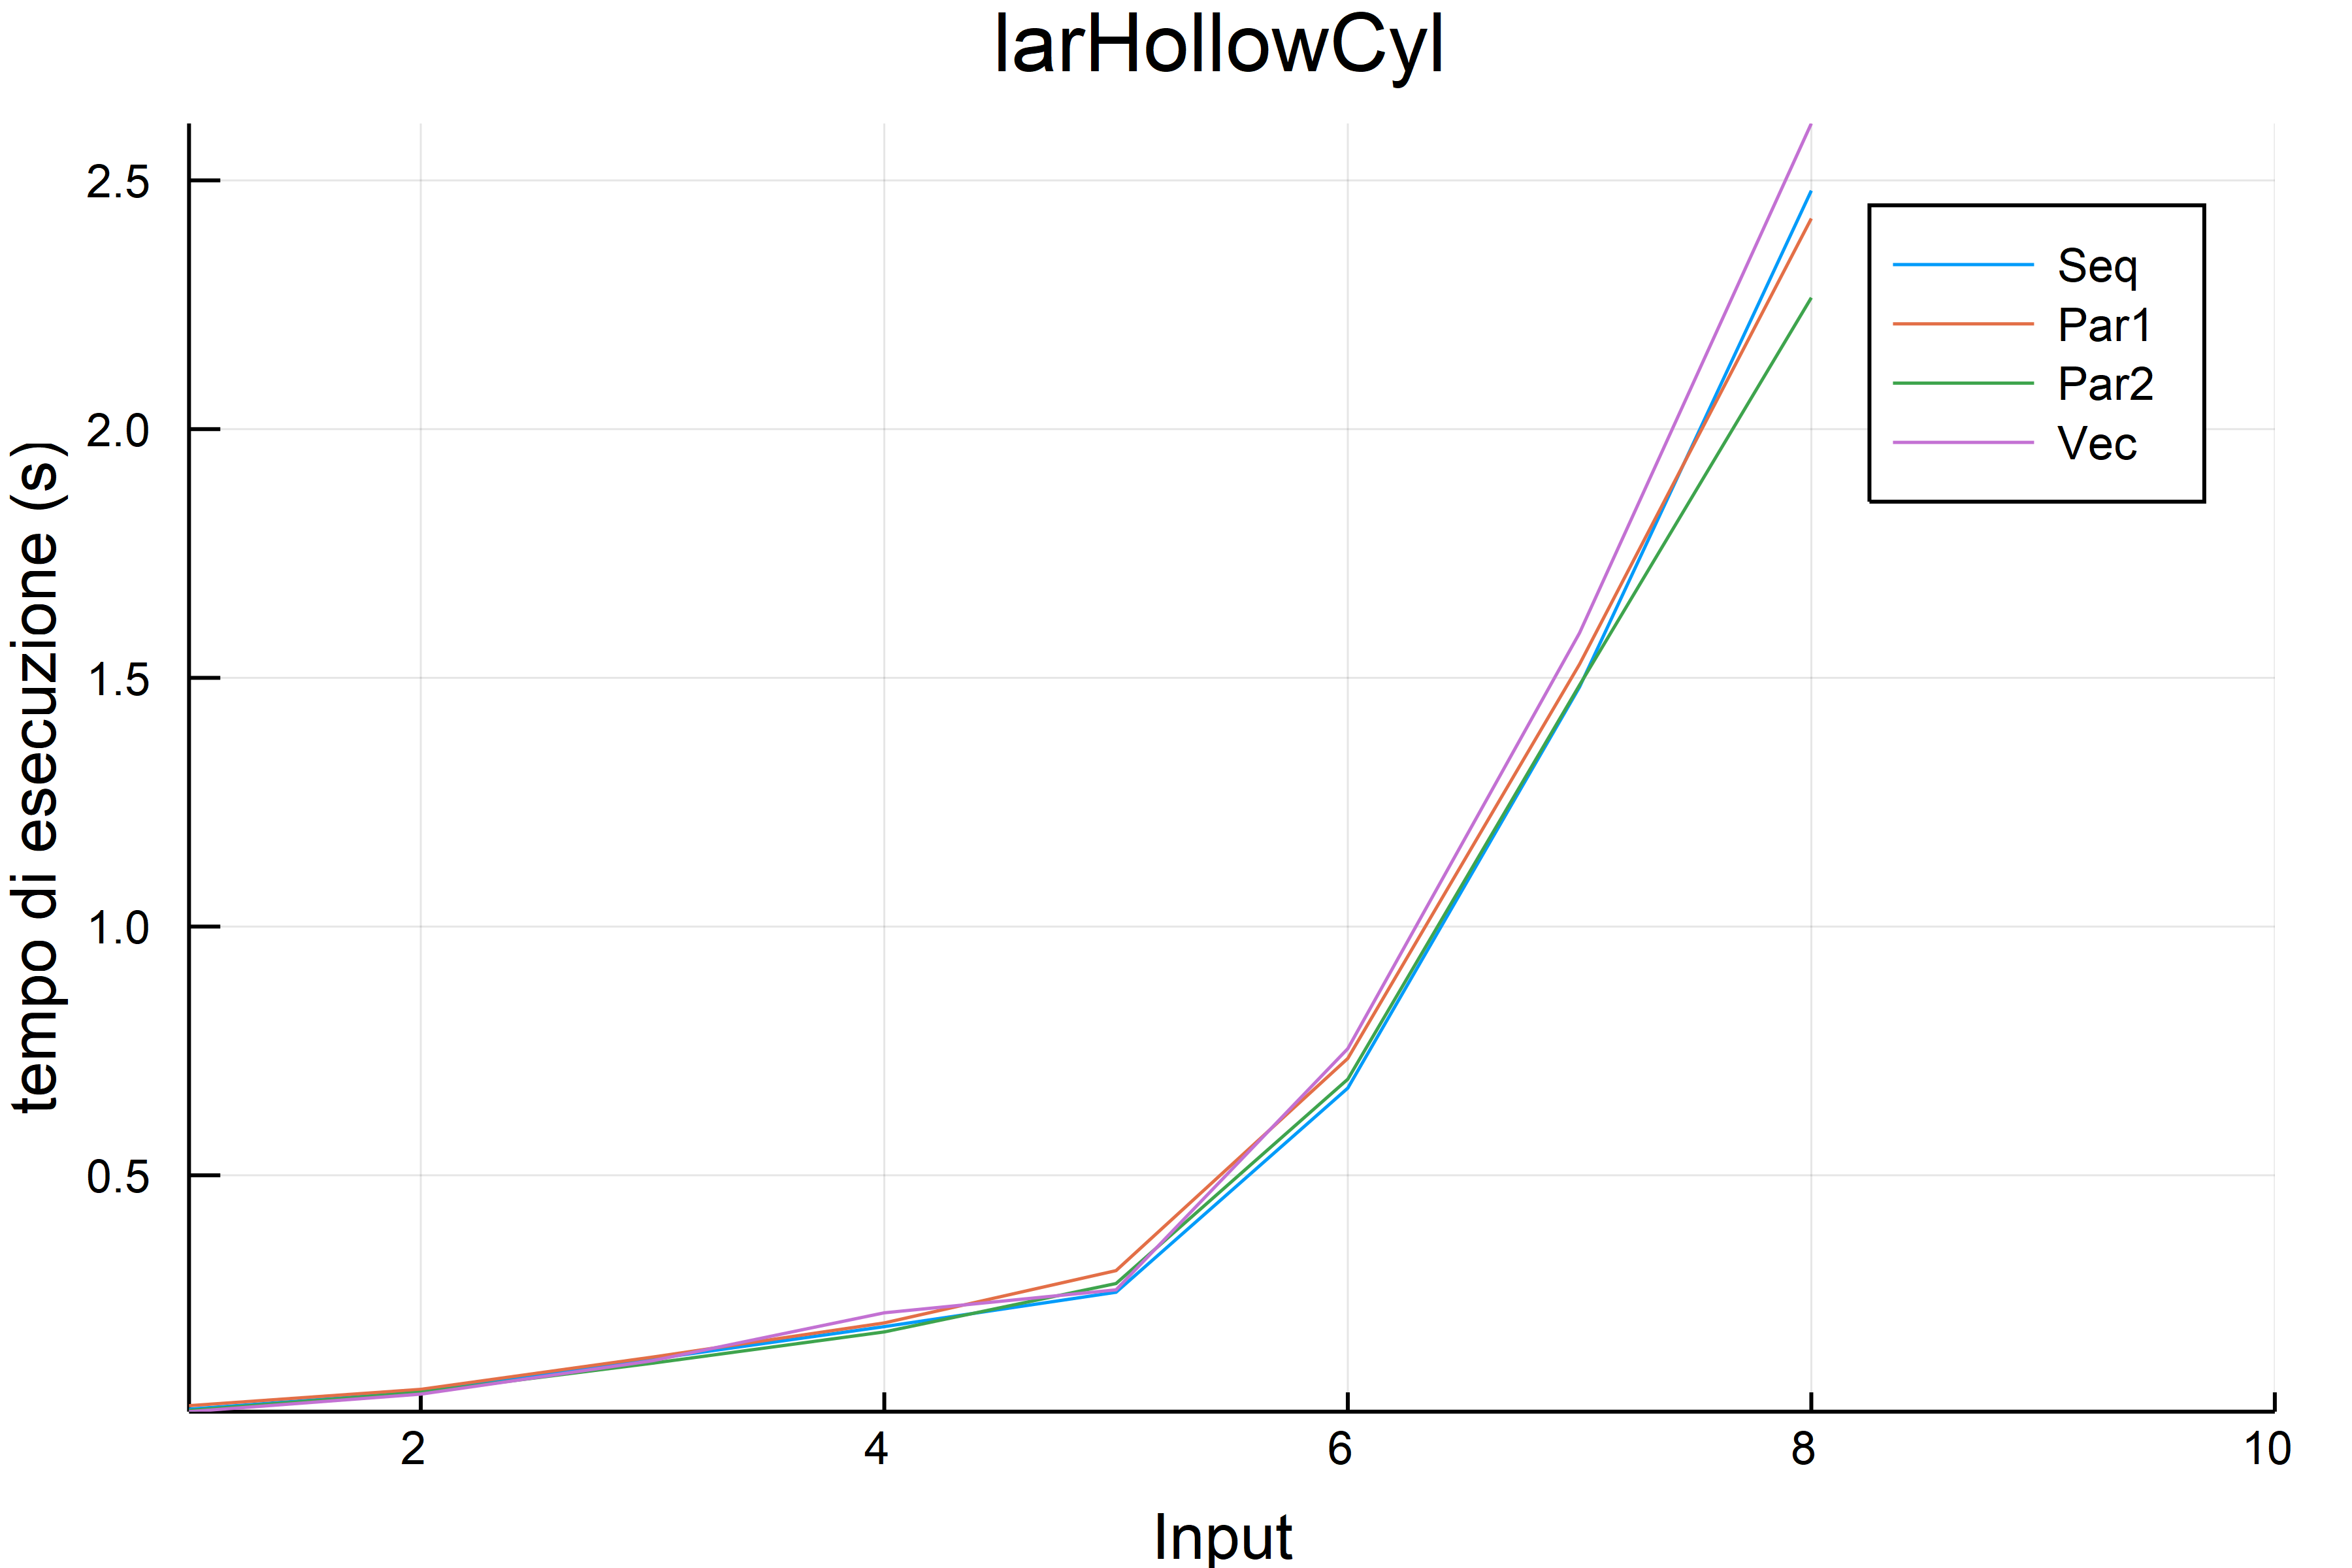
\includegraphics[scale=.13]{larHollowCylTime.png} 
\caption{Results computed on Microsoft Surface Pro  3 (4GB LPDDR3 1600 MHz RAM, i5-4300U processor)} 
\end{figure}
%---------------------------------------------------------------------------------
\subsection{larHollowSphere}

\paragraph{Python}

\begin{verbatim}
def larHollowSphere(r,R,angle1=PI,angle2=2*PI):
    def larHollowSphere0(shape=[36,1,1]):
        V,CV = larIntervals(shape)([angle1,angle2,R-r])
        V = larTranslate([-angle1/2,-angle2/2,r])(V)
        domain = V,CV
        x = lambda p : p[2]*COS(p[0])*COS(p[1])
        y = lambda p : p[2]*COS(p[0])*SIN(p[1])
        z = lambda p : p[2]*SIN(p[0])
        return larMap([x,y,z])(domain)
    return larHollowSphere0
\end{verbatim}

\paragraph{Julia}

\begin{verbatim}
function larHollowSphere(r,R,angle1=pi,angle2=2*pi)
    function larHollowSphere0(shape=[36,1,1])
        V,CV = LARLIB.larCuboids(shape)
        V = [angle1/shape[1] 0 0;0 angle2/shape[2] 0;0 0 (R-r)/shape[3]]*V
        V = broadcast(+,V,[-(angle1)/2,-(angle2)/2,r])
        W = [V[:,k] for k=1:size(V,2)]
        X = hcat(map(p->let(u,v,z)=p;[z*cos(u)*cos(v);z*cos(u)*sin(v);
        	z*sin(u)] end,W)...)
        return X,CV
    end
    return larHollowSphere0
end
\end{verbatim}

The \textfb{larHollowSphere} function creates an hollow sphere with given radiuses and angles.

In this case, the local parametrization used is:
$$f(u,v,z)=(zcos(u)cos(v);zcos(u)sin(v);zsin(u)),$$
with $[u,v,z] \in [-\frac{angle1}{2},\frac{angle1}{2}]\times[-\frac{angle2}{2},\frac{angle2}{2}]\times[r,R]$.

With $$\verb!V=broadcast(+,V,[-angle1/2,-angle2/2,r])!$$ we sum $-\frac{angle_1}{2}$ to each element in the first row of V, $-\frac{angle_2}{2}$ to each element in the second row of V and r to every element in the third row of V.

With $$\verb!W=[V[:,k] for k=1:size(V,2)]!,$$ as opposed to $hcat$, we dispose the coordinates of the vertices (i.e. the columns in V) horizontally (into an array of arrays).

Then $map$ applies the "anonymous function" $$\verb!p->let(u,v,z)=p;[z*cos(u)*cos(v);z*cos(u)*sin(v);z*sin(u)]end!$$ to the coordinates of all the vertices contained in the W collection. Next, with the $hcat$ function, the coordinates of the new vertices are rearranged vertically in a matrix.

\paragraph{Visualization example}

\begin{verbatim}
V,CV = larHollowSphere(1,2,pi,pi)([36,36,1])
V
CV
V = hcat(V[:,1],[V[:,k] for k in 1:size(V,2)]...)
W = [Any[V[h,k] for h=1:size(V,1)] for k=1:size(V,2)]
hpc = p.STRUCT(p.MKPOLS(PyObject([W,CV,[]])))
p.VIEW(hpc)
\end{verbatim}

\begin{figure}[htbp] 
\centering 
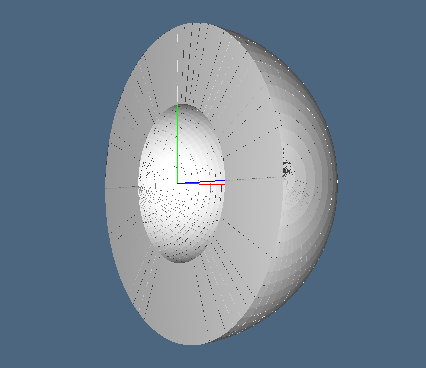
\includegraphics[scale=.38]{larHollowSphere.png} 
\caption{Half hollow sphere centered in the origin of radiuses 1 and 2.} 
\end{figure}

\paragraph{Test}

\begin{Verbatim}
@testset "larHollowSphere" begin
	@test BoxCalculation(larHollowSphere(0,2,pi,2*pi)([36,36,1])[1])==64
	@test BoxCalculation(larHollowSphere(1,6,pi,pi)([36,36,1])[1])==864
	@test BoxCalculation(larHollowSphere(2,4,pi,2*pi)([36,36,1])[1])==8^3
	#(radius*2)^3
	@test size(larHollowSphere(1.5,6.7,pi/3,2*pi/3)()[1],2)==148
	@test length(larHollowSphere(1.5,6.7,pi/3,2*pi/3)()[2])==36
end
\end{Verbatim}

\paragraph{Vectorization}

\begin{verbatim}
function larHollowSphereV(r,R,angle1=pi,angle2=2*pi)
    function larHollowSphere0(shape=[36,1,1])
        V,CV = LARLIB.larCuboids(shape)
        V = [V[:,k] for k=1:size(V,2)]
        V = (x->[x[1]*angle1/shape[1], x[2]*angle2/shape[2], x[3]*(R-r)/shape[3]]).(V)
        W = (p->[p[3]*cos(p[1])*cos(p[2]);p[3]*cos(p[1])*sin(p[2])
            ;p[3]*sin(p[1])]).((x->x+[-(angle1)/2,-(angle2)/2,r]).(V))
        return hcat(W...),CV
    end
    return larHollowSphere0
end
\end{verbatim}

\paragraph{Parallel Computing}
\begin{Verbatim}
function larHollowSphereP(r,R,a1=pi,a2=2*pi)
    function larHollowSphere0(s=[36,1,1])
        V,CV = LARLIB.larCuboids(s)
        W=SharedArray{Float64}(3,size(V,2))
            @sync @parallel for i=1:size(W,2)
                W[1,i] = (((V[3,i]*(R-r)/s[3])+r)*
                cos((V[1,i]*a1/s[1])-(a1/2))*cos((V[2,i]*a2/s[2])-(a2/2)))
                W[2,i] = (((V[3,i]*(R-r)/s[3])+r)*
                cos((V[1,i]*a1/s[1])-(a1/2))*sin((V[2,i]*a2/s[2])-(a2/2)))
                W[3,i] = (((V[3,i]*(R-r)/s[3])+r)*sin((V[1,i]*a1/s[1])-(a1/2)))
            end
       return W,CV
    end
    return larHollowSphere0
end
\end{Verbatim}

\begin{Verbatim}
@everywhere function flarHollowSphere(W::SharedArray,V::Array,indexprt,ultim,
            shape,r,R,angle1,angle2)
    id = myid()
    if id != nprocs()
        for i=indexprt*(id-2) +1 : indexprt*(id-1)
            W[1,i] = (((V[3,i]*(R-r)/shape[3])+r)*cos((V[1,i]*angle1/shape[1])-
            (angle1/2))*cos((V[2,i]*angle2/shape[2])-(angle2/2)))
            W[2,i] = (((V[3,i]*(R-r)/shape[3])+r)*cos((V[1,i]*angle1/shape[1])-
            (angle1/2))*sin((V[2,i]*angle2/shape[2])-(angle2/2)))
            W[3,i] = (((V[3,i]*(R-r)/shape[3])+r)*sin((V[1,i]*
            angle1/shape[1])-(angle1/2)))
        end
    else
        for i=indexprt*(id-2) +1 : ultim
            W[1,i] = (((V[3,i]*(R-r)/shape[3])+r)*cos((V[1,i]*angle1/shape[1])-(angle1/2))*
            cos((V[2,i]*angle2/shape[2])-(angle2/2)))
            W[2,i] = (((V[3,i]*(R-r)/shape[3])+r)*cos((V[1,i]*angle1/shape[1])-
            (angle1/2))*sin((V[2,i]*angle2/shape[2])-(angle2/2)))
            W[3,i] = (((V[3,i]*(R-r)/shape[3])+r)*sin((V[1,i]*
            angle1/shape[1])-(angle1/2)))
        end
    end
end

function larHollowSpherePP(r,R,angle1=pi,angle2=2*pi)
    function larHollowSphere0(shape=[36,1,1])
        V,CV = LARLIB.larCuboids(shape)
        W=SharedArray{Float64}(3,size(V,2))
        if nprocs() > size(V,2)
            indexprt = 1
        else
            indexprt = Int((size(V,2)-(size(V,2)%nprocs()))/nprocs())
        end
        @sync begin
            for i = 2:nprocs()
                @async remotecall_fetch(flarHollowSphere,i,W,V,indexprt,size(V,2),
                shape,r,R,angle1,angle2)
            end
        end
       return W,CV
    end
    return larHollowSphere0
end
\end{Verbatim}

\begin{Verbatim}
@testset "Vectorized and Parallelized larHollowSphere" begin
    @test BoxCalculation(larHollowSphereV(0,2,pi,2*pi)([36,36,1])[1])==64
    @test BoxCalculation(larHollowSphereP(1,6,pi,pi)([36,36,1])[1])==864
    @test BoxCalculation(larHollowSpherePP(2,4,pi,2*pi)([36,36,1])[1])==8^3
    @test BoxCalculation(larHollowSphereP(0,2,pi,2*pi)([36,36,1])[1])==64
    @test BoxCalculation(larHollowSpherePP(1,6,pi,pi)([36,36,1])[1])==864
    @test BoxCalculation(larHollowSphereP(2,4,pi,2*pi)([36,36,1])[1])==8^3
end
\end{Verbatim}

\paragraph{Performance evaluation}

\begin{Verbatim}
data = [[x,1,1] for x in data2]

x,y = TimeGraph(larHollowSphere(1,2),larHollowSphereP(1,2),larHollowSpherePP(1,2),larHollowSphereV(1,2),data,5)
plot(x,y,yaxis=("tempo di esecuzione (s)"),xaxis=("Input",(1,length(x)+2)),
label=["Seq" "Par1" "Par2" "Vec"],title="larHollowSphere",lw=1)

\end{Verbatim}

\begin{figure}[htbp] 
\centering 
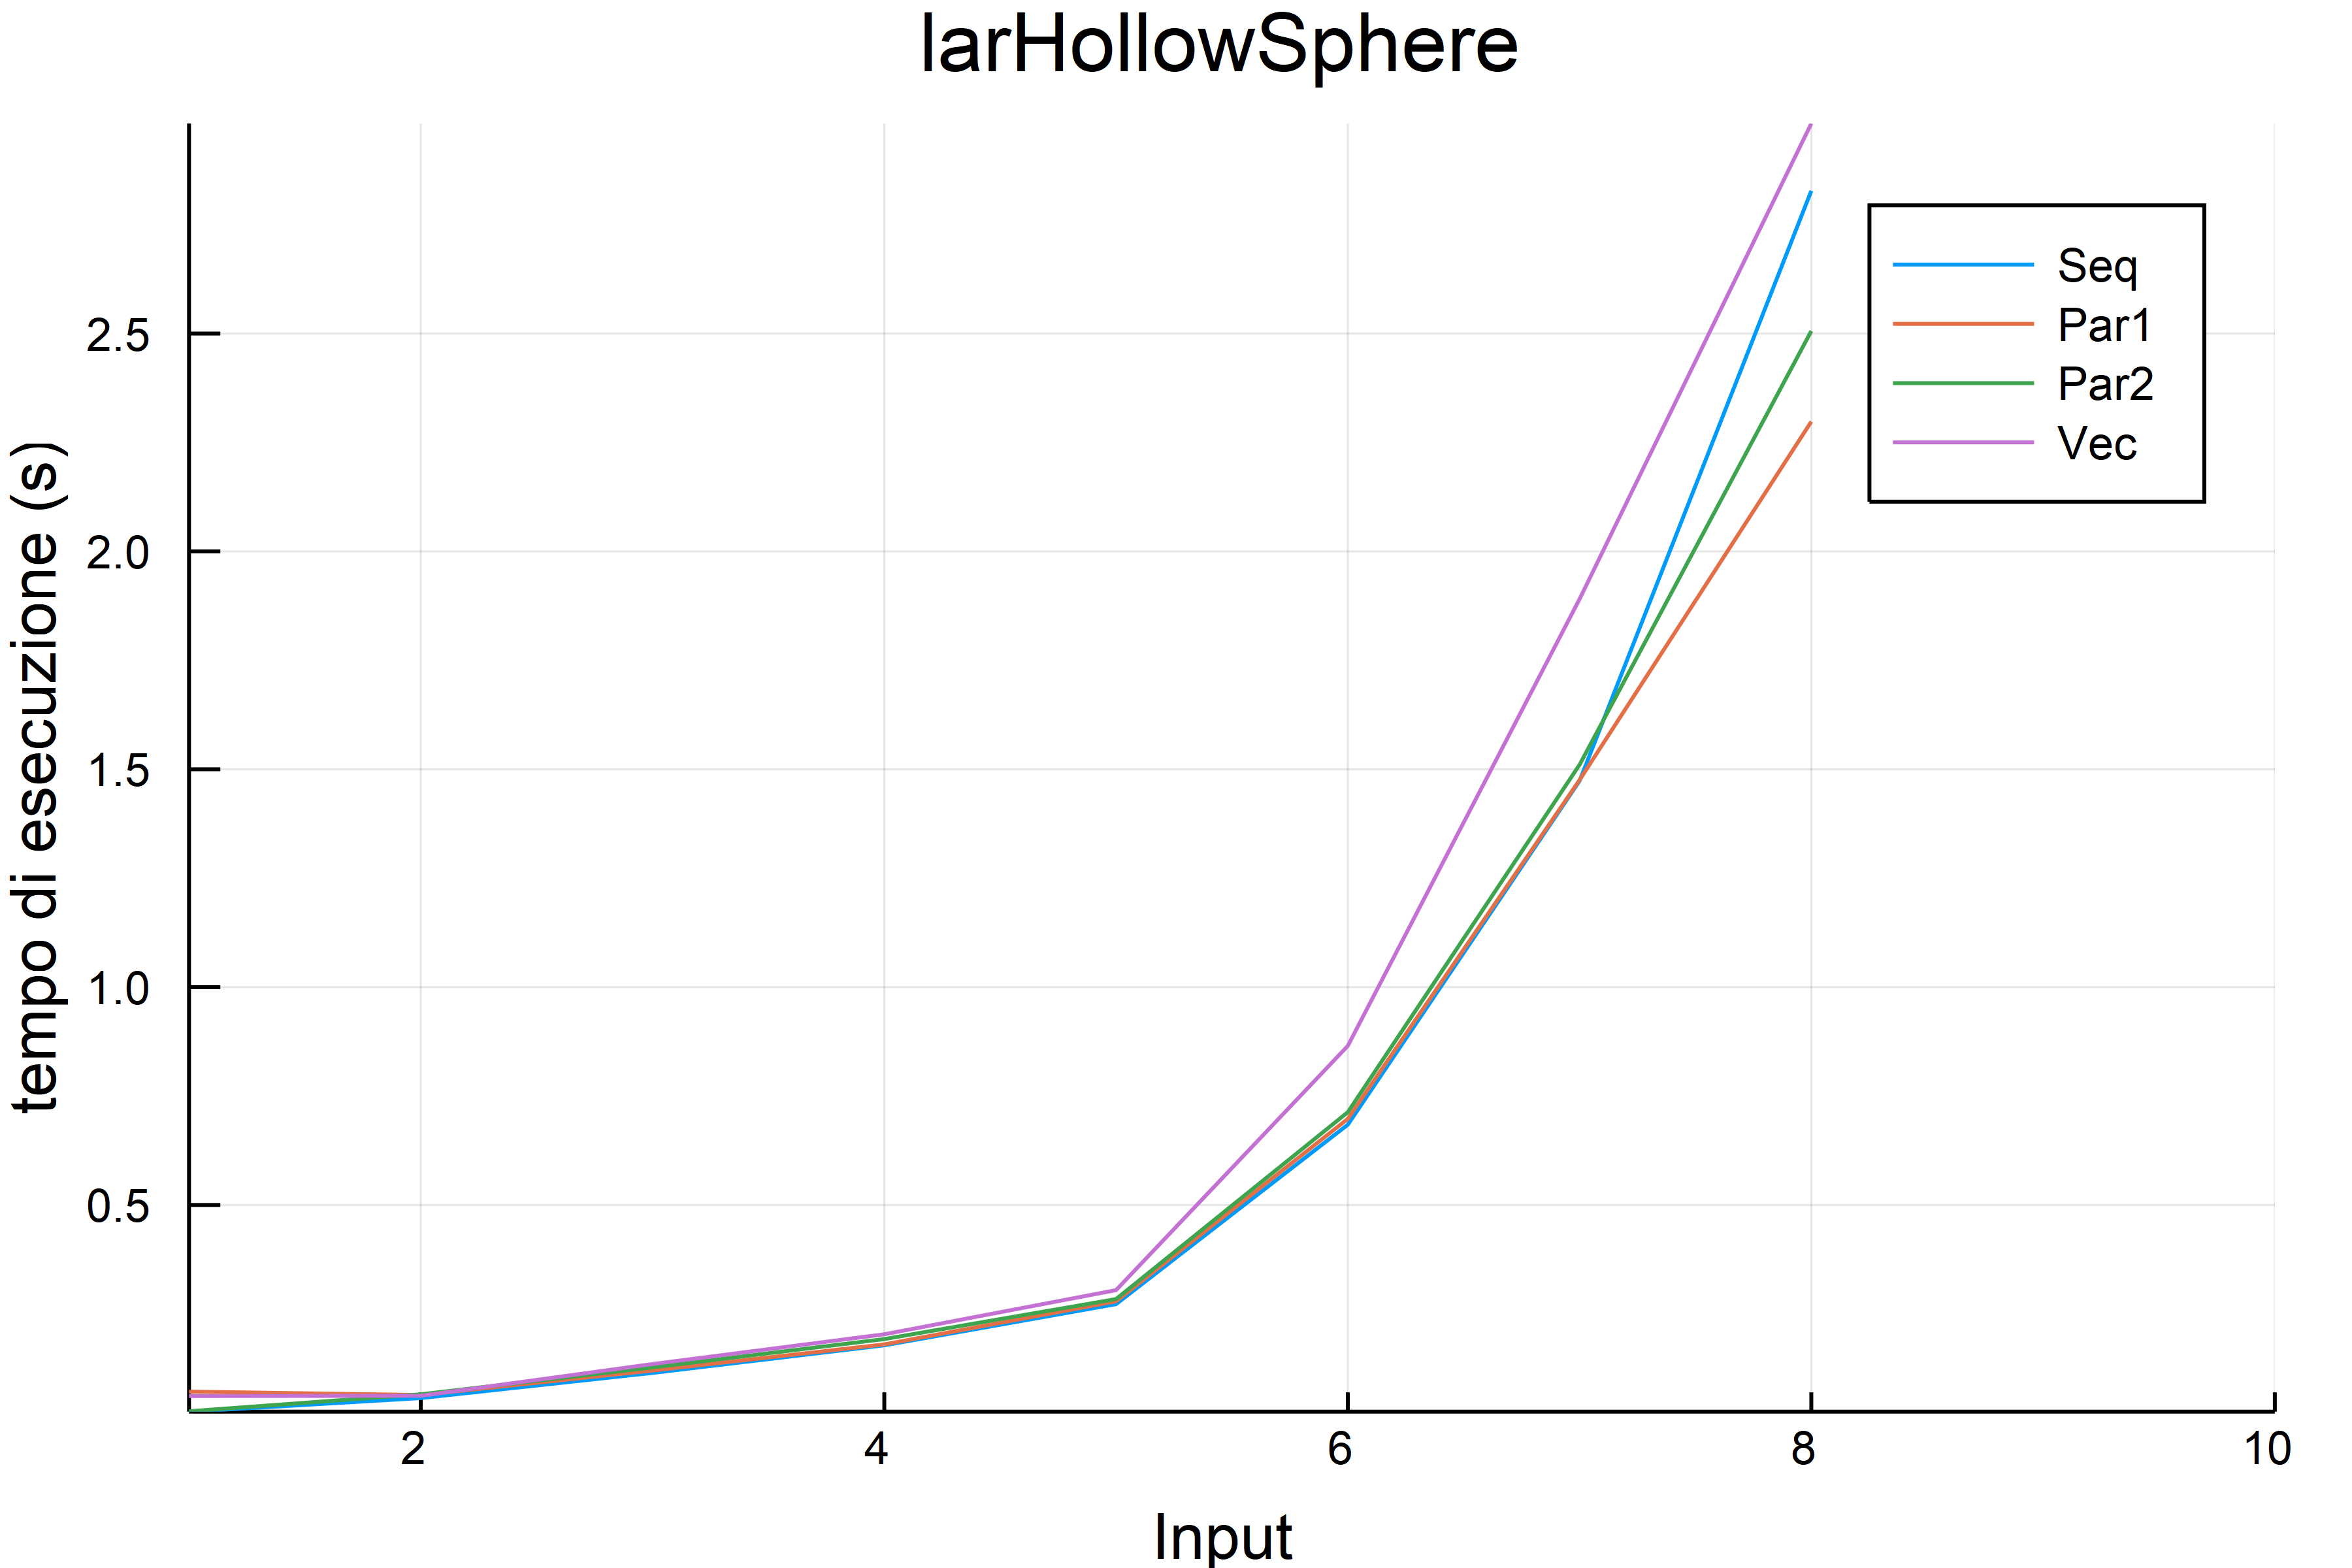
\includegraphics[scale=.13]{larHollowSphereTime.png} 
\caption{Results computed on Microsoft Surface Pro  3 (4GB LPDDR3 1600 MHz RAM, i5-4300U processor)} 
\end{figure}

%---------------------------------------------------------------------------------
\subsection{larTorus}

\paragraph{Python}

\begin{verbatim}
def larTorus(r,R,angle1=2*PI,angle2=2*PI):
    def larTorus0(shape=[24,36,1]):
        domain = larIntervals(shape)([angle1,angle2,r])
        V,CV = domain
        x = lambda p : (R + p[2]*COS(p[0])) * COS(p[1])
        y = lambda p : (R + p[2]*COS(p[0])) * SIN(p[1])
        z = lambda p : -p[2] * SIN(p[0])
        return larMap([x,y,z])(domain)
    return larTorus0
\end{verbatim}

\paragraph{Julia}

\begin{verbatim}
function larTorus(r,R,angle1=2*pi,angle2=2*pi)
    function larTorus0(shape=[24,36,1])
        V,CV = LARLIB.larCuboids(shape)
        V = [angle1/shape[1] 0 0;0 angle2/shape[2] 0;0 0 r/shape[3]]*V
        W = [V[:,k] for k=1:size(V,2)]
        X = hcat(map(p->let(u,v,z)=p;[(R+z*cos(u))*cos(v);(R+z*cos(u))*sin(v);
        	-z*sin(u)] end,W)...)
       return X,CV
    end
    return larTorus0
end
\end{verbatim}

The \textfb{larTorus} function creates a solid torus with given radiuses (radius of the circumference that generates it and distance from origin) and angle.

In this case, the local parametrization used is:
$$f(u,v,z)=((R+zcos(u))cos(v);(R+zcos(u))sin(v);-zsin(u)),$$ 
with $[u,v,z] \in [0,angle1]\times[0,angle2]\times[0,r]$.

With $$\verb!W=[V[:,k] for k=1:size(V,2)]!,$$ as opposed to $hcat$, we dispose the coordinates of the vertices (i.e. the columns in V) horizontally (into an array of arrays).

Then $map$ applies the "anonymous function" $$\verb!p->let(u,v,z)=p;[(R+z*cos(u))*cos(v);(R+z*cos(u))*sin(v);-z*sin(u)]end!$$ to the coordinates of all the vertices contained in the W collection. Next, with the $hcat$ function, the coordinates of the new vertices are rearranged vertically in a matrix.

\paragraph{Visualization examples}

\begin{verbatim}
V,CV = larTorus(1,3,2*pi,2*pi)()
V
CV
V = hcat(V[:,1],[V[:,k] for k in 1:size(V,2)]...)
W = [Any[V[h,k] for h=1:size(V,1)] for k=1:size(V,2)]
hpc = p.STRUCT(p.MKPOLS(PyObject([W,CV,[]])))
p.VIEW(hpc)

V,CV = larTorus(1,3,pi,2*pi)()
V = hcat(V[:,1],[V[:,k] for k in 1:size(V,2)]...)
W = [Any[V[h,k] for h=1:size(V,1)] for k=1:size(V,2)]
hpc = p.STRUCT(p.MKPOLS(PyObject([W,CV,[]])))
p.VIEW(hpc)
\end{verbatim}

\begin{figure}[htbp] 
\centering 
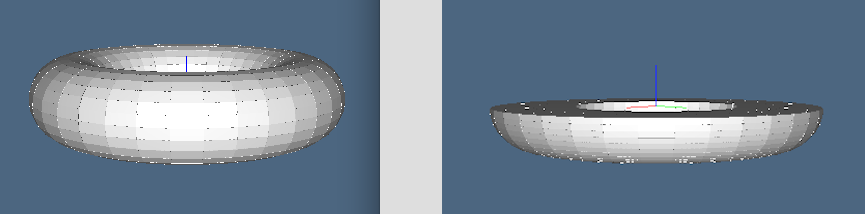
\includegraphics[scale=.44]{larTorus.png} 
\caption{Solid torus centered in the origin and its horizontal section, of radiuses 1 and 3.} 
\end{figure}

\paragraph{Test}
\begin{Verbatim}
@testset "larTorus" begin
	@test BoxCalculation(larTorus(1,3,2*pi,2*pi)()[1])==128
	@test BoxCalculation(larTorus(2,3,2*pi,2*pi)()[1])==400
	#(((R+r)*2)^2)*(r*2)
	@test size(larTorus(5.2,7,pi/3,pi/4)()[1],2)==1850
	@test length(larTorus(5.2,7,pi/3,pi/4)()[2])==864
end
\end{Verbatim}

\paragraph{Vectorization}

\begin{verbatim}
function larTorusV(r,R,angle1=2*pi,angle2=2*pi)
    function larTorus0(shape=[24,36,1])
        V,CV = LARLIB.larCuboids(shape)
        V = [V[:,k] for k=1:size(V,2)]
        W = (p->[(R+p[3]*cos(p[1]))*cos(p[2]);(R+p[3]*cos(p[1]))*sin(p[2]);
            -p[3]*sin(p[1])]).((x->[x[1]*angle1/shape[1],x[2]*angle2/shape[2], x[3]*r/shape[3]]).(V))
       return hcat(W...),CV
    end
    return larTorus0
end
\end{verbatim}

\paragraph{Parallel Computing}
\begin{Verbatim}
function larTorusP(r,R,angle1=2*pi,angle2=2*pi)
    function larTorus0(shape=[24,36,1])
        V,CV = LARLIB.larCuboids(shape)
        V = SharedArray(V)
        W = SharedArray{Float64}(3,size(V,2))           
        @sync @parallel for i = 1:size(V,2)
            W[1,i] = (R+(V[3,i]*r/shape[3])*cos(V[1,i]*angle1/shape[1]))*
            cos(V[2,i]*angle2/shape[2])       
            W[2,i] = (R+(V[3,i]*r/shape[3])*cos(V[1,i]*angle1/shape[1]))*
            sin(V[2,i]*angle2/shape[2])
            W[3,i] = -(V[3,i]*r/shape[3])*sin(V[1,i]*angle1/shape[1])
        end
        return W,CV
    end
    return larTorus0
end 
\end{Verbatim}

\begin{Verbatim}
@everywhere function flarTorus(W::SharedArray,V::Array,indexprt,ultim,
            shape,r,R,angle1,angle2)
    id = myid()
    if id != nprocs()
        for i=indexprt*(id-2) +1 : indexprt*(id-1)
            W[1,i] = (R+(V[3,i]*r/shape[3])*cos(V[1,i]*angle1/shape[1]))*
            cos(V[2,i]*angle2/shape[2])       
            W[2,i] = (R+(V[3,i]*r/shape[3])*cos(V[1,i]*angle1/shape[1]))*
            sin(V[2,i]*angle2/shape[2])
            W[3,i] = -(V[3,i]*r/shape[3])*sin(V[1,i]*angle1/shape[1])
        end
    else
        for i=indexprt*(id-2) +1 : ultim
            W[1,i] = (R+(V[3,i]*r/shape[3])*cos(V[1,i]*angle1/shape[1]))*
            cos(V[2,i]*angle2/shape[2])       
            W[2,i] = (R+(V[3,i]*r/shape[3])*cos(V[1,i]*angle1/shape[1]))*
            sin(V[2,i]*angle2/shape[2])
            W[3,i] = -(V[3,i]*r/shape[3])*sin(V[1,i]*angle1/shape[1])
        end
    end
end

function larTorusPP(r,R,angle1=2*pi,angle2=2*pi)
    function larTorus0(shape=[24,36,1])
        V,CV = LARLIB.larCuboids(shape)
        W = SharedArray{Float64}(3,size(V,2))           
        if nprocs() > size(V,2)
            indexprt = 1
        else
            indexprt = Int((size(V,2)-(size(V,2)%nprocs()))/nprocs())
        end
        @sync begin
            for i = 2:nprocs()
                @async remotecall_fetch(flarTorus,i,W,V,indexprt,size(V,2),
                shape,r,R,angle1,angle2)
            end
        end
        return W,CV
    end
    return larTorus0
end 
\end{Verbatim}

\begin{Verbatim}
@testset "Vectorized and Parallelized larTorus" begin
    @test BoxCalculation(larTorusV(1,3,2*pi,2*pi)()[1])==128
    @test BoxCalculation(larTorusV(2,3,2*pi,2*pi)()[1])==400
    @test BoxCalculation(larTorusPP(1,3,2*pi,2*pi)()[1])==128
    @test BoxCalculation(larTorusPP(2,3,2*pi,2*pi)()[1])==400
    @test BoxCalculation(larTorusP(1,3,2*pi,2*pi)()[1])==128
    @test BoxCalculation(larTorusP(2,3,2*pi,2*pi)()[1])==400
end
\end{Verbatim}

\paragraph{Performance evaluation}

\begin{Verbatim}
data = [[x,1,1] for x in data2]

x,y = TimeGraph(larTorus(1,2),larTorusP(1,2),larTorusPP(1,2),larTorusV(1,2),data,5)
plot(x,y,yaxis=("tempo di esecuzione (s)"),xaxis=("Input",(1,length(x)+2)),
label=["Seq" "Par1" "Par2" "Vec"],title="larTorus",lw=1)

\end{Verbatim}

\begin{figure}[htbp] 
\centering 
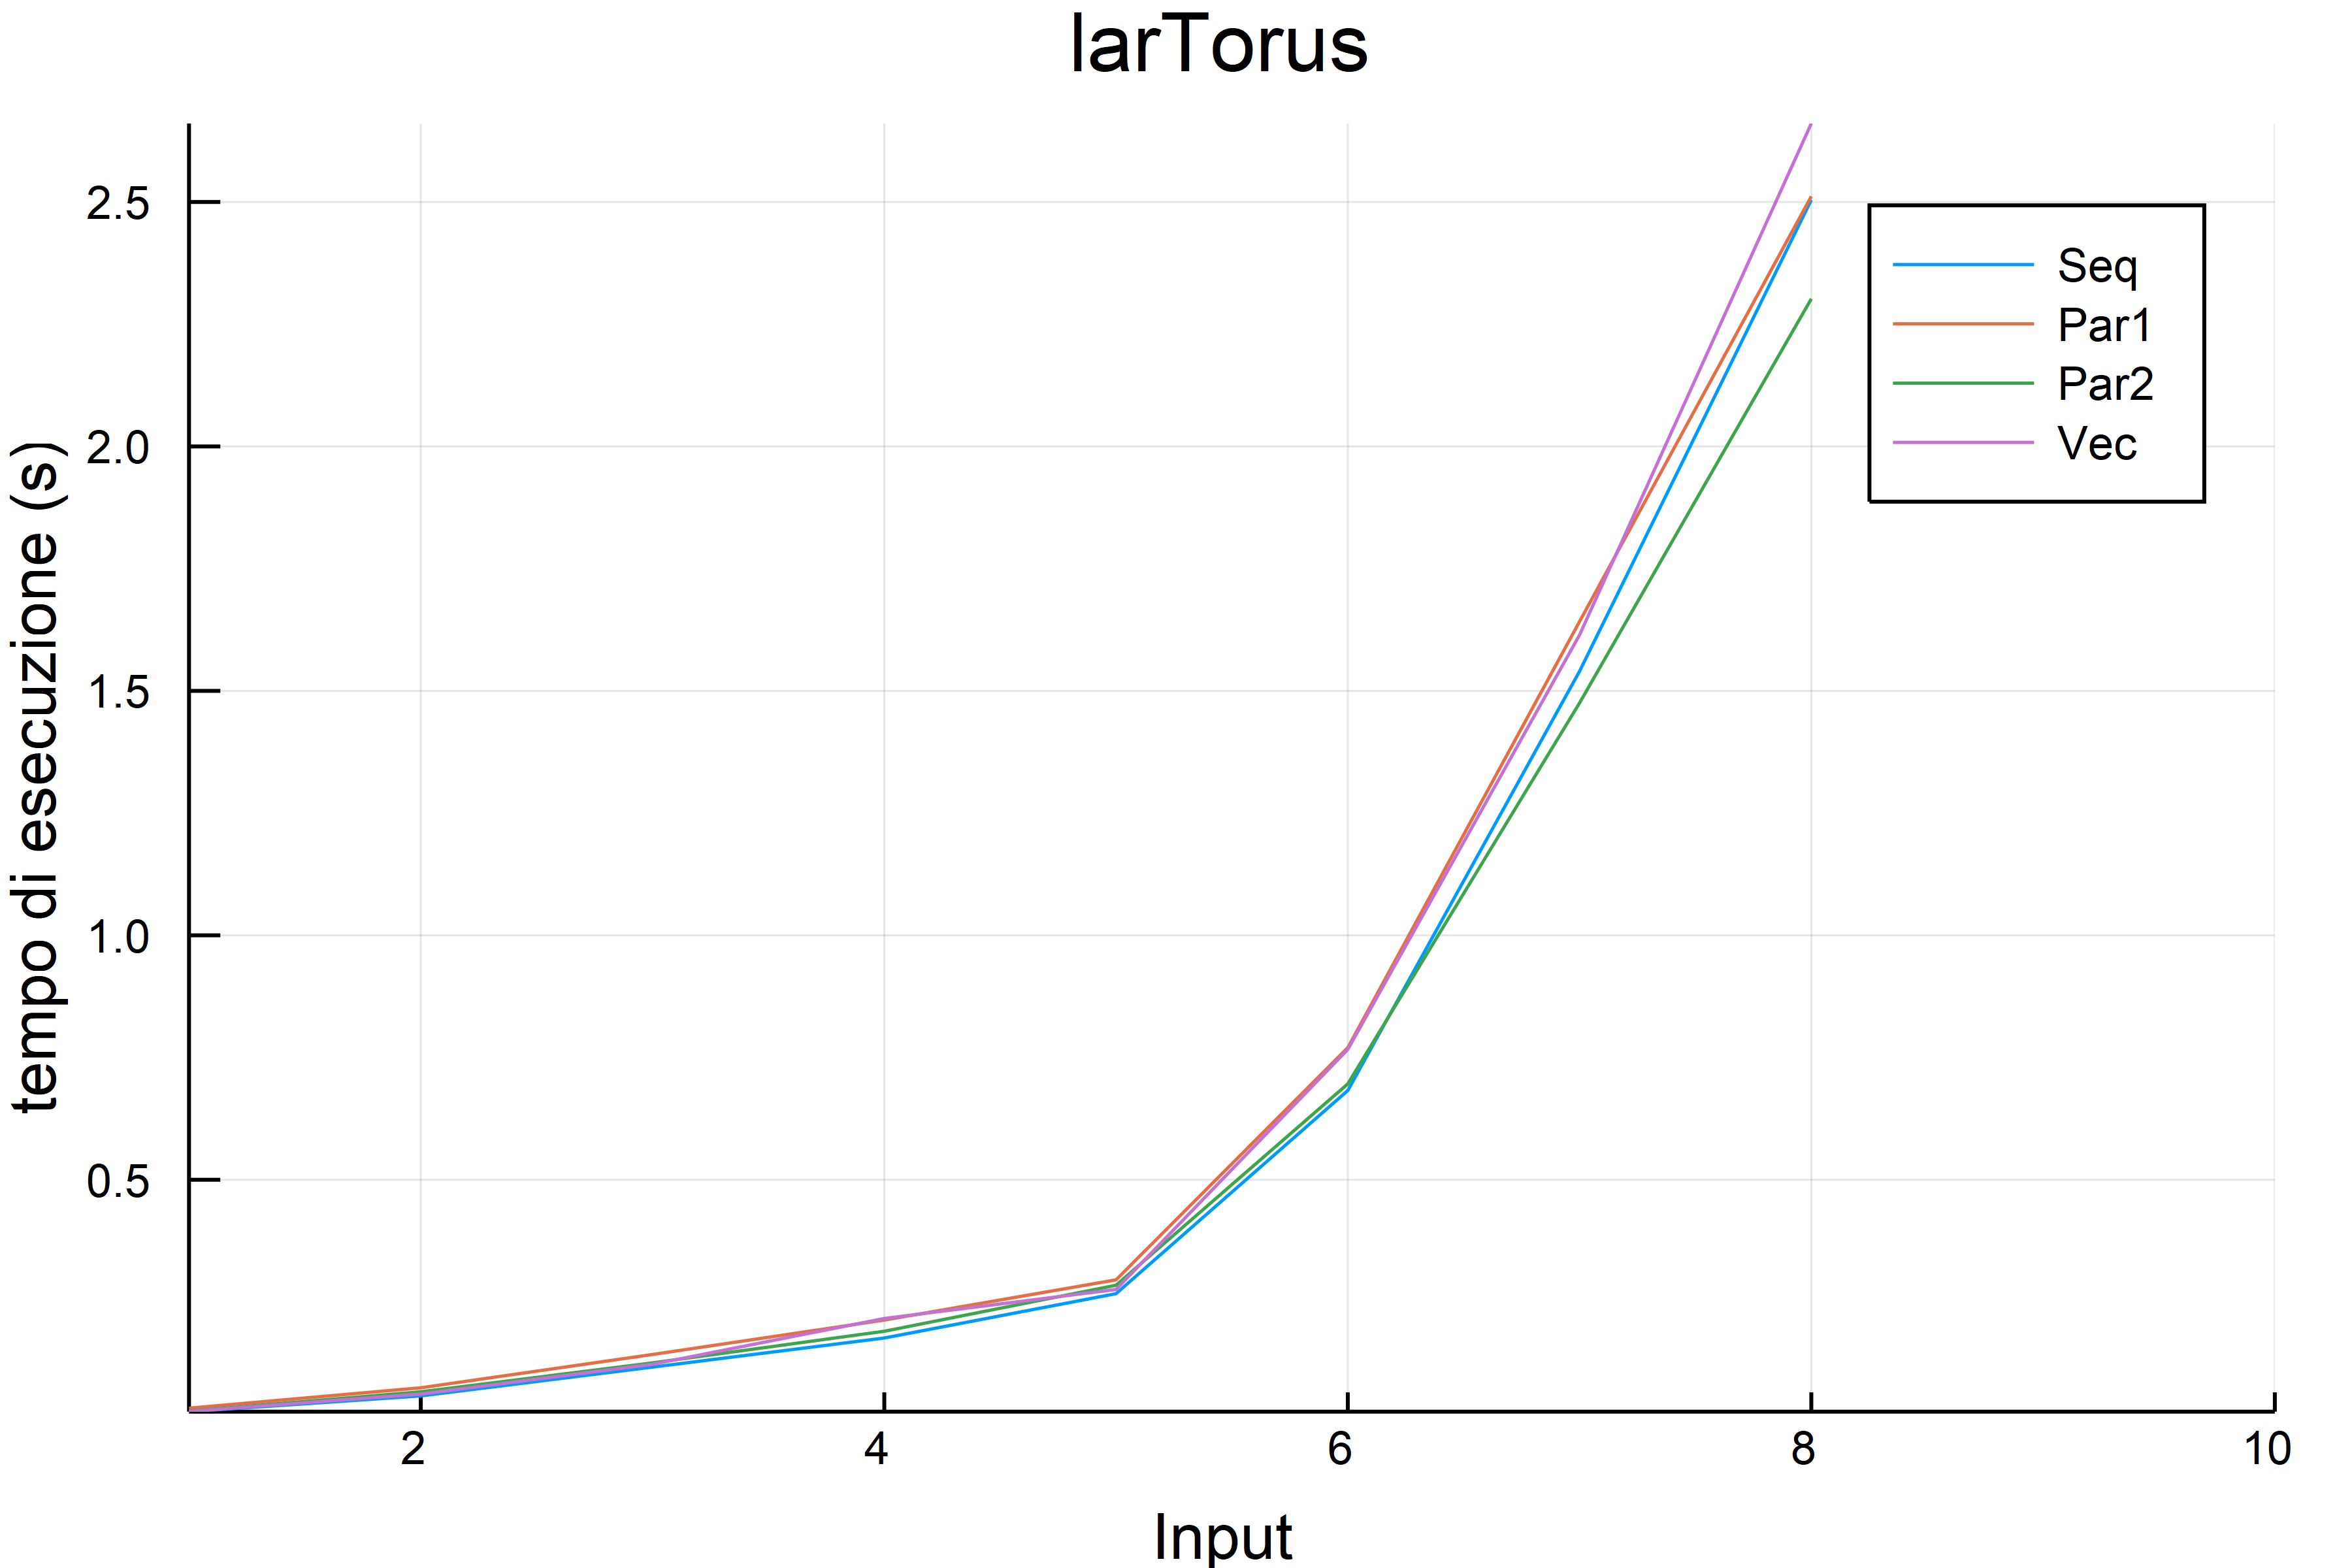
\includegraphics[scale=.13]{larTorusTime.png} 
\caption{Results computed on Microsoft Surface Pro  3 (4GB LPDDR3 1600 MHz RAM, i5-4300U processor)} 
\end{figure}
%---------------------------------------------------------------------------------
\subsection{larPizza}

\paragraph{Python}

\begin{verbatim}
def larPizza(r,R,angle=2*PI):
    assert angle <= PI
    def larPizza0(shape=[24,36]):
        V,CV = checkModel(larCrown(r,R,angle)(shape))
        V += [[0,0,-r],[0,0,r]]
        return V,[range(len(V))]
    return larPizza0
\end{verbatim}

\paragraph{Julia}

\begin{verbatim}
function larPizza(r,R,angle=pi)
    function larPizza0(shape=[24,36])
        V,CV = larCrown(r,R,angle)(shape)
        W = [Any[V[h,k] for h=1:size(V,1)] for k=1:size(V,2)]
        W = [map(approxVal(4),v) for v in W]
        X = hcat(collect(Set(W))...)
        H = hcat(X,[0 0;0 0;-r r])
        return H,[collect(0:size(H,2)-1)]
    end
    return larPizza0
end
\end{verbatim}

The \textbf{larPizza} function creates a pizza shaped solid, with given radiuses and angle.

The model to "fill" is generated with $$\verb!V,CV = larCrown(r,R,angle)(shape)!$$. In this case, a larCrown.

With $$\verb!W = [Any[V[h,k] for h = 1:size(V,1)] for k = 1:size(V,2)]!,$$ as opposed to $hcat$, we dispose the coordinates of the vertices (i.e. the columns in V) horizontally (into an array of arrays).

With $$\verb!W = [map(approxVal(4),v) for v in W]!$$ we round every element of each array in W to the fourth decimal place.

\verb!Set(W)! deletes the doubles in W and saves them in a set, with $collect$ this collection is turned back into an array of arrays: the elements are the coordinates of the sphere vertices.
With the $hcat$ function the coordinates of the vertices just created are arranged vertically in a matrix.

With \verb!H = hcat(X,[0 0;0 0;-r r])! we add, at the end of the X matrix, the submatrix: 
\[
\begin{bmatrix}
0 & 0 \\
0 & 0 \\
-r & r
\end{bmatrix}
\]
Named \verb!n=size(H,2)! the number of columns in H, then the function returns the matrix H of the vertices and the array $[0,1,2,3,...,n-1]$.

\paragraph{Visualization examples}

\begin{verbatim}
V,CV = larPizza(0.2,4,pi/3)()
V
CV
W = [Any[V[h,k] for h=1:size(V,1)] for k=1:size(V,2)]
hpc = p.STRUCT(p.MKPOLS(PyObject([W,CV,[]])))
p.VIEW(hpc)
\end{verbatim}

\begin{figure}[htbp] 
\centering 
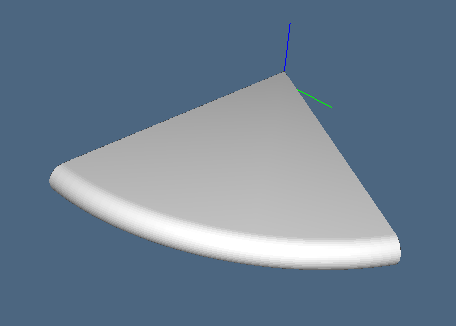
\includegraphics[scale=.42]{larPizza.png} 
\caption{"pizza" solid centered in the origin, with a 60 degree angle and radiuses of 0.2 and 4.} 
\end{figure}

\paragraph{Test}
\begin{Verbatim}
@testset "larPizza" begin
	@test BoxCalculation(larPizza(1,2,pi/2)()[1])==18
	@test BoxCalculation(larPizza(0.5,2,pi)()[1])==12.5
	#(((R+r)*2)^2)*r se angolo=pi
	@test size(larPizza(0.03,5.6,pi/9)()[1],2)==927
	@test length(larPizza(0.03,5.6,pi/9)()[2])==1
end
\end{Verbatim}

\paragraph{Vectorization\\}
\begin{Verbatim}
function larPizzaV(r,R,angle=pi)
    function larPizza0(shape=[24,36])
        V,CV = larCrown(r,R,angle)(shape)
        V = approxVal(4).(V)
        W = hcat(collect(Set([V[:,k] for k=1:size(V,2)]))...)
        W = hcat(W,[0 0;0 0;-r r])
        return W,[collect(0:size(W,2)-1)]
    end
    return larPizza0
end
\end{Verbatim}

\paragraph{Parallel Computing\\}

\begin{Verbatim}
function larPizzaP(r,R,angle=pi)
    function larPizza0(shape=[24,36])
        V,CV=larCrownP(r,R,angle)(shape)
        V = SharedArray(V)
        @sync @parallel for i = 1:size(V,2)
            V[1,i] = approxVal(4)(V[1,i])
            V[2,i] = approxVal(4)(V[2,i])
            V[3,i] = approxVal(4)(V[3,i])
        end
        W = hcat(collect(Set([V[:,k] for k=1:size(V,2)]))...)
        W=hcat(W,[0 0;0 0;-r r])
        return W,[collect(0:size(W,2)-1)]
    end
    return larPizza0
end
\end{Verbatim}

\begin{Verbatim}
function larPizzaPP(r,R,angle=pi)   #sembra la più veloce
    function larPizza0(shape=[24,36])
        V,CV=larCrownP(r,R,angle)(shape)
        V = SharedArray(V)
        if nprocs() > size(V,2)
            indexprt = 1
        else
            indexprt = Int((size(V,2)-(size(V,2)%nprocs()))/nprocs())
        end
        @sync begin
            for i = 2:nprocs()
                @async remotecall_fetch(fP,i,V,indexprt,size(V,2))
            end
        end
        W = hcat(collect(Set([V[:,k] for k=1:size(V,2)]))...)
        W=hcat(W,[0 0;0 0;-r r])
        return W,[collect(0:size(W,2)-1)]
    end
    return larPizza0
end
\end{Verbatim}

\begin{Verbatim}
@testset "Vectorized and Parallelized larPizza" begin
	@test BoxCalculation(larPizzaV(1,2,pi/2)()[1])==18
	@test BoxCalculation(larPizzaV(0.5,2,pi)()[1])==12.5
	@test BoxCalculation(larPizzaPP(1,2,pi/2)()[1])==18
	@test BoxCalculation(larPizzaPP(0.5,2,pi)()[1])==12.5
	@test BoxCalculation(larPizzaP(1,2,pi/2)()[1])==18
	@test BoxCalculation(larPizzaP(0.5,2,pi)()[1])==12.5
end
\end{Verbatim}

\paragraph{Performance evaluation}

\begin{Verbatim}
data = [[x,1] for x in data3]

x,y = TimeGraph(larPizza(1,2),larPizzaP(1,2),larPizzaPP(1,2),larPizzaV(1,2),data,5)
plot(x,y,yaxis=("tempo di esecuzione (s)"),xaxis=("Input",(1,length(x)+2)),
label=["Seq" "Par1" "Par2" "Vec"],title="larPizza",lw=1)

\end{Verbatim}

\begin{figure}[htbp] 
\centering 
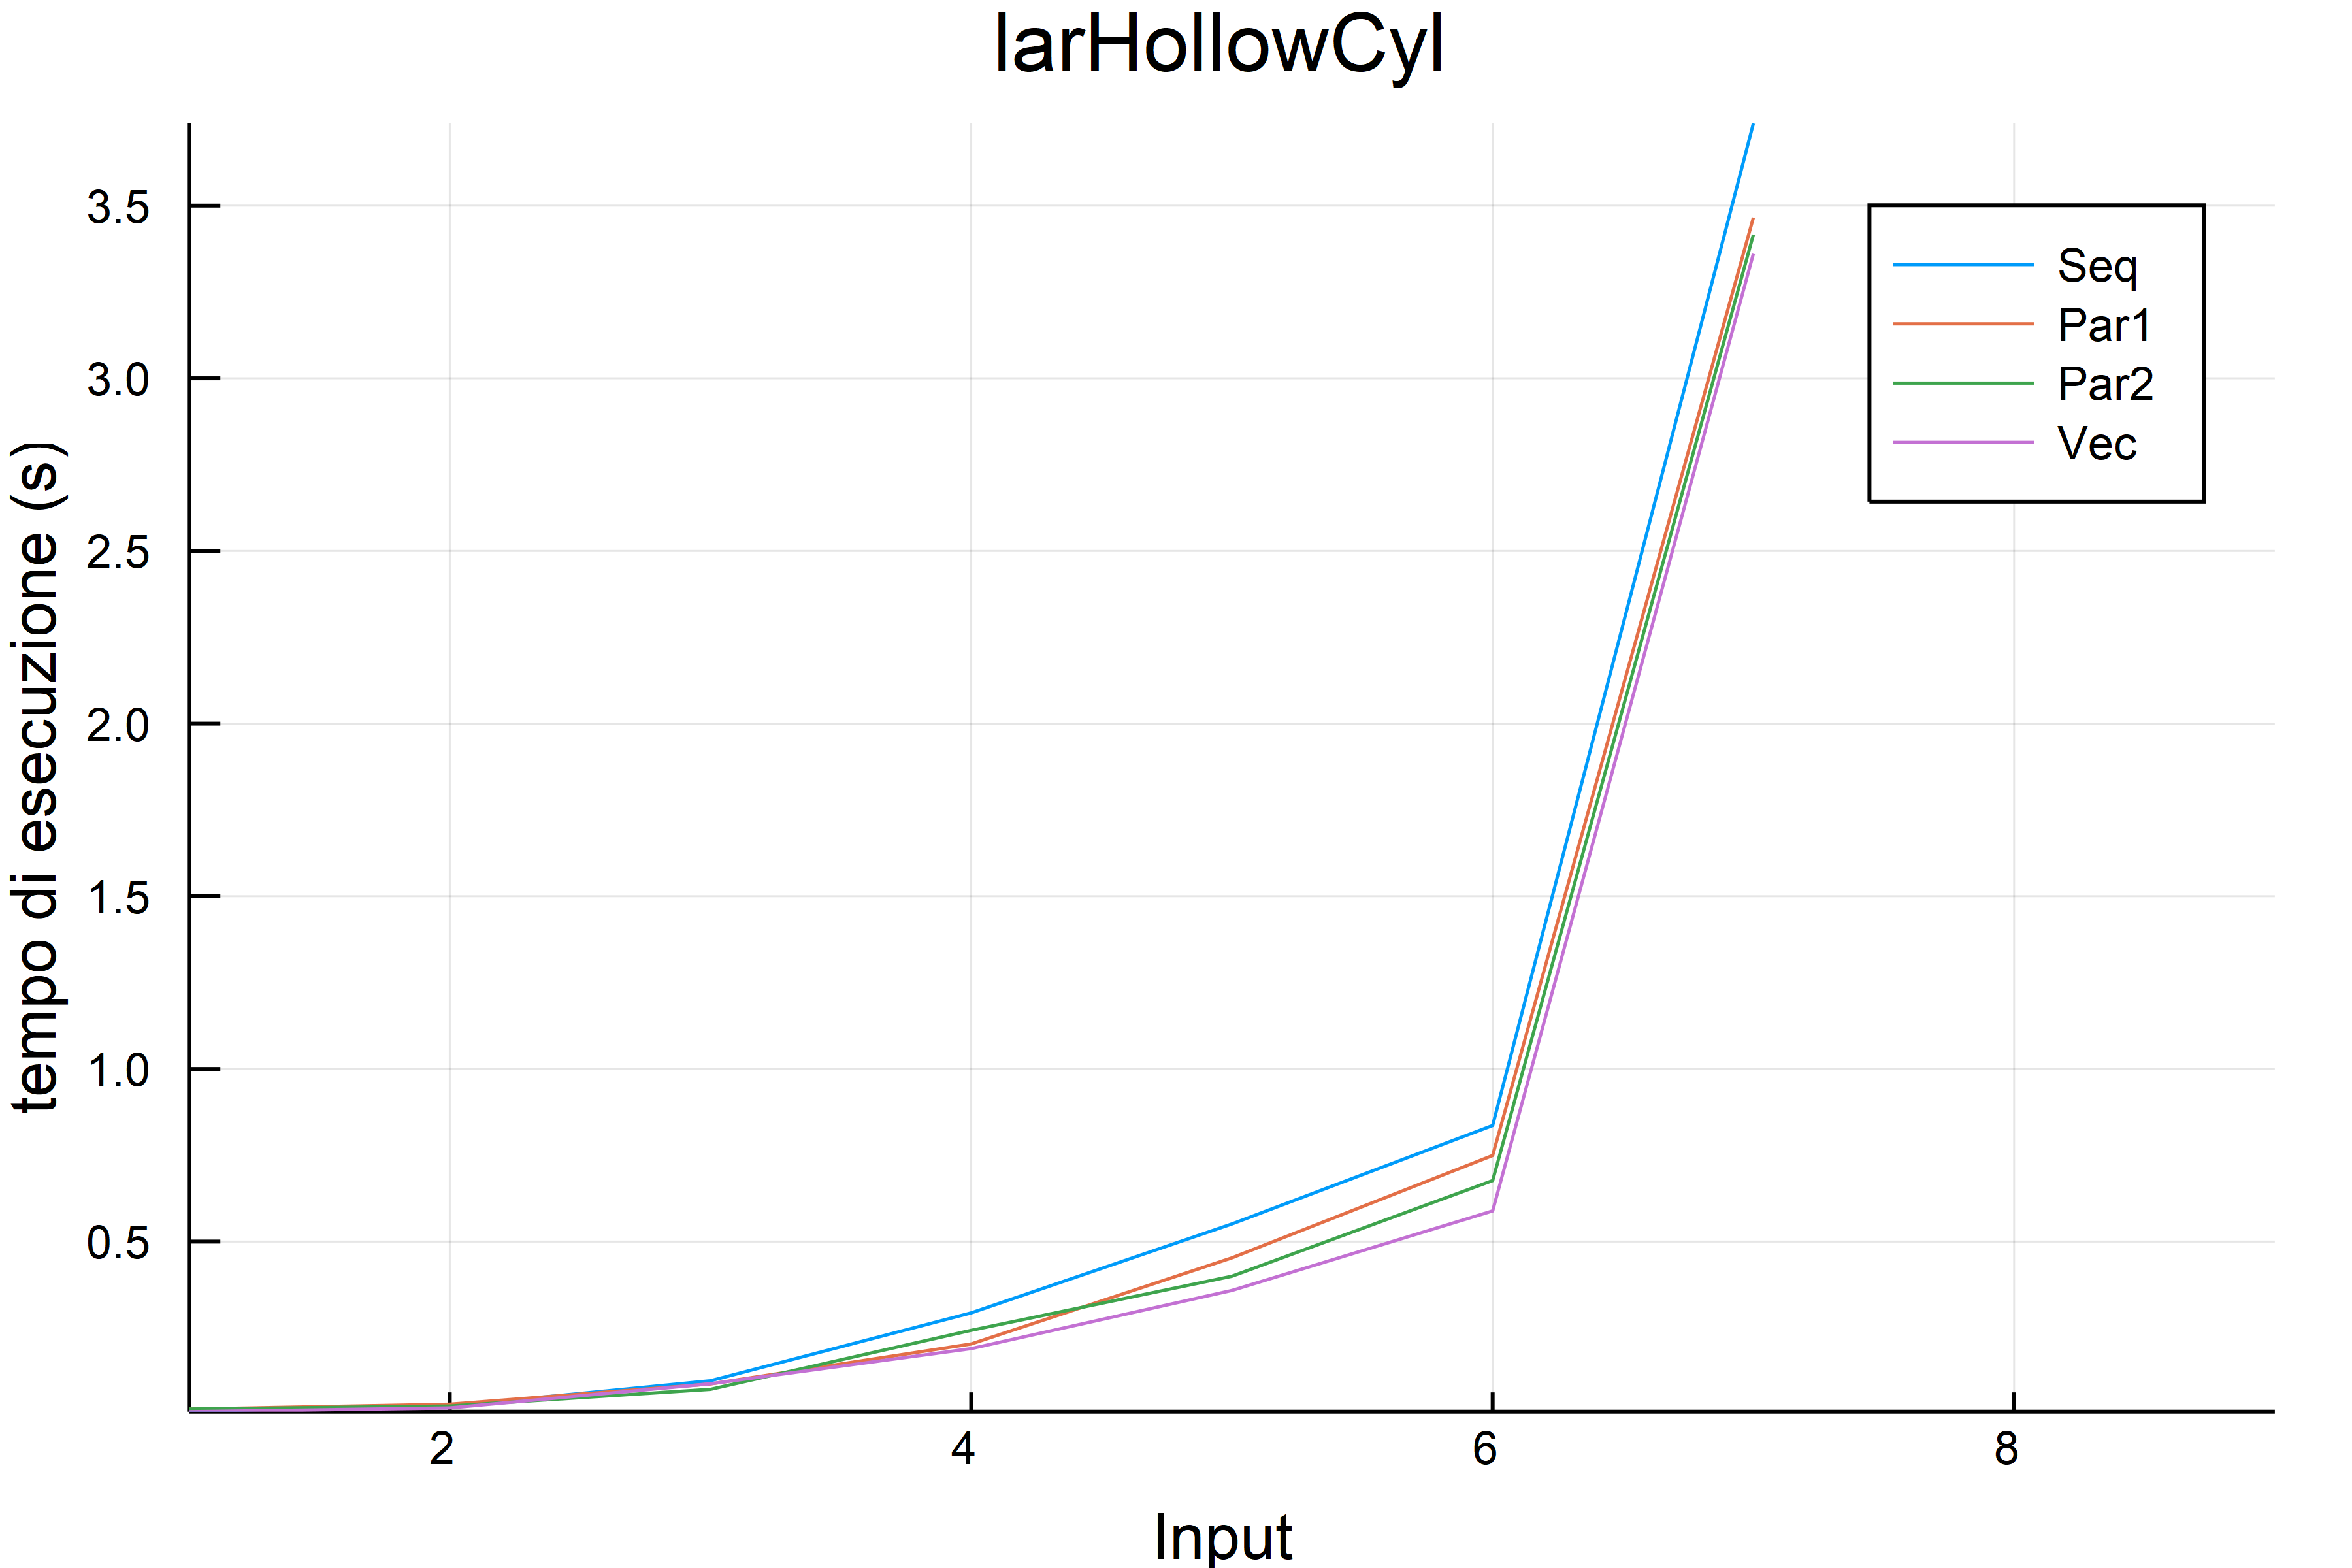
\includegraphics[scale=.13]{larPizzaTime.png} 
\caption{Results computed on Microsoft Surface Pro  3 (4GB LPDDR3 1600 MHz RAM, i5-4300U processor)} 
\end{figure}

%=================================================================================

\newpage
\section{Conclusions}

To conclude, let's calculate the speed up. The speed up is given by the ratio between the serial function execution time and the parallel function execution time

$$S_p = \frac{T_s(n) }{T_p(n)}, $$ where n is the size of input and p is the number of processors.

A speed up greater than one means that the parallel algorithm is faster. Usually the parallelization makes sense when a process works on a huge quantity of data, performing complex operations on them multiple times. On the contrary, if instead the algorithm works on a small amount of data, the parallelization could be inopportune, with the risk of slowing down the execution due to the scheduling needed to assign the work to the processors, and without real benefits.

\begin{Verbatim}

p = 8

input1 = [10000,50000,100000,500000]

input2 = [1000,5000,10000,50000]

input3 = [5000,10000,50000,100000]

#larCircle 

speedUpP = [TimeCalculate(larCircle(),n,1)/
                    TimeCalculate(larCircleP(),n,1) for n in input1]

speedUpPP = [TimeCalculate(larCircle(),n,1)/
                    TimeCalculate(larCirclePP(),n,1) for n in input1]

#larHelix

speedUpP = [TimeCalculate(larHelix(),n,1)/
                    TimeCalculate(larHelixP(),n,1) for n in input1]

speedUpPP = [TimeCalculate(larHelix(),n,1)/
                    TimeCalculate(larHelixPP(),n,1) for n in input1]

#larDisk

speedUpP = [TimeCalculate(larDisk(),[n,1],1)/
                    TimeCalculate(larDiskP(),[n,1],1) for n in input1]

speedUpPP = [TimeCalculate(larDisk(),[n,1],1)/
                    TimeCalculate(larDiskPP(),[n,1],1) for n in input1]

#larHelicoid

speedUpP = [TimeCalculate(larHelicoid(),[n,1],1)/
                    TimeCalculate(larHelicoidP(),[n,1],1) for n in input2]

speedUpPP = [TimeCalculate(larHelicoid(),[n,1],1)/
                    TimeCalculate(larHelicoidPP(),[n,1],1) for n in input2]

#larRing

speedUpP = [TimeCalculate(larRing(1,2),[n,1],1)/
                    TimeCalculate(larRingP(1,2),[n,1],1) for n in input1]

speedUpPP = [TimeCalculate(larRing(1,2),[n,1],1)/
                    TimeCalculate(larRingPP(1,2),[n,1],1) for n in input1]

#larCylinder

speedUpP = [TimeCalculate(larCylinder(1,2),[n,1],1)/
                    TimeCalculate(larCylinderP(1,2),[n,1],1) for n in input1]

speedUpPP = [TimeCalculate(larCylinder(1,2),[n,1],1)/
                    TimeCalculate(larCylinderPP(1,2),[n,1],1) for n in input1]

#larSphere

speedUpP = [TimeCalculate(larSphere(),[n,1],1)/
                    TimeCalculate(larSphereP(),[n,1],1) for n in input2]

speedUpPP = [TimeCalculate(larSphere(),[n,1],1)/
                    TimeCalculate(larSpherePP(),[n,1],1) for n in input2]

#larToroidal

speedUpP = [TimeCalculate(larToroidal(),[n,1],1)/
                    TimeCalculate(larToroidalP(),[n,1],1) for n in input2]

speedUpPP = [TimeCalculate(larToroidal(),[n,1],1)/
                    TimeCalculate(larToroidalPP(),[n,1],1) for n in input2]

#larCrown

speedUpP = [TimeCalculate(larCrown(),[n,1],1)/
                    TimeCalculate(larCrownP(),[n,1],1) for n in input2]

speedUpPP = [TimeCalculate(larCrown(),[n,1],1)/
                    TimeCalculate(larCrownPP(),[n,1],1) for n in input2]

#larBall

speedUpP = [TimeCalculate(larBall(),[n,1],1)/
                    TimeCalculate(larBallP(),[n,1],1) for n in input3]

speedUpPP = [TimeCalculate(larBall(),[n,1],1)/
                    TimeCalculate(larBallPP(),[n,1],1) for n in input3]

#larRod

speedUpP = [TimeCalculate(larRod(),[n,1],1)/
                    TimeCalculate(larRodP(),[n,1],1) for n in input1]

speedUpPP = [TimeCalculate(larRod(),[n,1],1)/
                    TimeCalculate(larRodPP(),[n,1],1) for n in input1]

#larHollowCyl

speedUpP = [TimeCalculate(larHollowCyl(1,2,1),[n,1,1],1)/
                        TimeCalculate(larHollowCylP(1,2,1),[n,1,1],1) for n in input1]

speedUpPP = [TimeCalculate(larHollowCyl(1,2,1),[n,1,1],1)/
                        TimeCalculate(larHollowCylPP(1,2,1),[n,1,1],1) for n in input1]

#larHollowShere

speedUpP = [TimeCalculate(larHollowSphere(1,2),[n,1,1],1)/
                        TimeCalculate(larHollowSphereP(1,2),[n,1,1],1)for n in input1]

speedUpPP = [TimeCalculate(larHollowSphere(1,2),[n,1,1],1)/
                        TimeCalculate(larHollowSpherePP(1,2),[n,1,1],1) for n in input1]

#larTorus

speedUpP = [TimeCalculate(larTorus(1,2),[n,1,1],1)/
                        TimeCalculate(larTorusP(1,2),[n,1,1],1) for n in input1]

speedUpPP = [TimeCalculate(larTorus(1,2),[n,1,1],1)/
                        TimeCalculate(larTorusPP(1,2),[n,1,1],1) for n in input1]

#larPizza

speedUpP = [TimeCalculate(larPizza(1,2),[n,1],1)/
                        TimeCalculate(larPizzaP(1,2),[n,1],1) for n in input3]

speedUpPP = [TimeCalculate(larPizza(1,2),[n,1],1)/
                        TimeCalculate(larPizzaPP(1,2),[n,1],1) for n in input3]

#larBox
 
speedUpP = [TimeCalculateLBox(larBox,rand(Int,n),rand(Int,n),1)/
                    TimeCalculateLBox(larBoxP,rand(Int,n),rand(Int,n),1) for n in [17,18,19,20]]
\end{Verbatim}

\paragraph{Results:}

\begin{Verbatim}

larCircle

speedUpP = [1.08215, 0.789292, 0.982552, 1.0891] 
speedUpPP = [0.964349, 0.920818, 1.0212, 1.04413]  

larHelix

speedUpP = [1.01609, 0.747712, 0.897625, 1.05163] 
speedUpPP = [2.72167, 0.80021, 1.05213, 1.02961]

larDisk

speedUpP = [0.935595, 1.00024, 0.994913, 1.06556] 
speedUpPP = [0.971795, 1.06335, 1.08361, 1.08477] 

larHelicoid

speedUpP = [1.06808, 0.951521, 0.964679, 1.02206] 
speedUpPP = [1.20443, 0.95508, 0.974648, 1.00785] 

larRing

speedUpP = [0.878624, 1.01928, 1.00382, 1.12182] 
speedUpPP = [0.972484, 1.00777, 1.02295, 1.13715] 
 
larCylinder

speedUpP = [2.37662, 0.987392, 1.08917, 1.09787] 
speedUpPP = [1.05461, 1.04897, 1.17017, 1.13344]

larSphere

speedUpP = [0.977831, 1.00993, 0.964086, 1.10265] 
speedUpPP = [0.727737, 0.967877, 0.99773, 1.03474]

larToroidal

speedUpP = [0.709744, 0.923217, 0.963044, 1.02388]
speedUpPP = [0.883679, 0.969851, 1.02042, 1.01052] 

larCrown

speedUpP = [0.799535, 0.901144, 0.979384, 1.00232] 
speedUpPP = [0.829869, 0.968052, 0.997196, 1.00723] 

larBall

speedUpP =  [0.804228, 0.965848, 1.01059, 1.02468] 
speedUpPP = [1.00445, 0.919268, 1.00111, 1.02712] 

larRod

speedUpP = [0.994716, 1.20125, 1.15765, 1.22764] 
speedUpPP = [0.981295, 1.10687, 1.25756, 1.28698]

larHollowCyl

speedUpP = [0.954713, 0.98145, 1.14187, 1.16403] 
speedUpPP = [1.0392, 1.07112, 1.10308, 1.20067]

larHollowSphere

speedUpP = [1.02244, 1.00595, 1.097217, 1.21299] 
speedUpPP = [1.03774, 1.14925, 1.11311, 1.22408]
 

larTorus

speedUpP =  [0.94324, 1.00117, 1.08403, 1.13517]
speedUpPP = [1.03444, 1.0011, 1.07869, 1.19929]

larPizza

speedUpP = [0.945128, 0.998935, 1.02623, 1.01828]
speedUpPP = [0.94413, 1.26115, 1.00621, 1.0036]


larBox
 
speedUpP = [0.544591, 0.595939, 0.596564, 0.596694]


\end{Verbatim}


From these data, we can notice that the execution times of the parallel functions are quite similar to the others.
Therefore we can conclude that in most cases the parallelization leads to a slight improvement, that is visible but not decisive.

\begin{thebibliography}{9} 
\addcontentsline{toc}{section}{References} 
\bibitem{1}\emph{The Julia Language - Documentation} 
\url{https://docs.julialang.org/en/v0.6.2/manual/documentation/} 
\bibitem{2}\emph{Domain mapping with LAR}
\url{https://github.com/cvdlab/lar-cc/blob/master/doc/pdf/mapper.pdf} 
\end{thebibliography} 
\end{document}